\documentclass{beamer}
\usepackage{amsmath}
\usepackage[english]{babel} %set language; note: after changing this, you need to delete all auxiliary files to recompile
\usepackage[utf8]{inputenc} %define file encoding; latin1 is the other often used option
\usepackage{csquotes} % provides context sensitive quotation facilities
\usepackage{graphicx} %allows for inserting figures
\usepackage{booktabs} % for table formatting without vertical lines
\usepackage{textcomp} % allow for example using the Euro sign with \texteuro
\usepackage{stackengine}
\usepackage{wasysym}
\usepackage{tikzsymbols}
\usepackage{textcomp}
\setbeamertemplate{navigation symbols}{}
\newcommand{\bubblethis}[2]{
        \tikz[remember picture,baseline]{\node[anchor=base,inner sep=0,outer sep=0]%
        (#1) {\underline{#1}};\node[overlay,cloud callout,callout relative pointer={(0.2cm,-0.7cm)},%
        aspect=2.5,fill=yellow!90] at ($(#1.north)+(-0.5cm,1.6cm)$) {#2};}%
    }%
\tikzset{face/.style={shape=circle,minimum size=4ex,shading=radial,outer sep=0pt,
        inner color=white!50!yellow,outer color= yellow!70!orange}}
%% Some commands to make the code easier
\newcommand{\emoticon}[1][]{%
  \node[face,#1] (emoticon) {};
  %% The eyes are fixed.
  \draw[fill=white] (-1ex,0ex) ..controls (-0.5ex,0.2ex)and(0.5ex,0.2ex)..
        (1ex,0.0ex) ..controls ( 1.5ex,1.5ex)and( 0.2ex,1.7ex)..
        (0ex,0.4ex) ..controls (-0.2ex,1.7ex)and(-1.5ex,1.5ex)..
        (-1ex,0ex)--cycle;}
\newcommand{\pupils}{
  %% standard pupils
  \fill[shift={(0.5ex,0.5ex)},rotate=80] 
       (0,0) ellipse (0.3ex and 0.15ex);
  \fill[shift={(-0.5ex,0.5ex)},rotate=100] 
       (0,0) ellipse (0.3ex and 0.15ex);}

\newcommand{\emoticonname}[1]{
  \node[below=1ex of emoticon,font=\footnotesize,
        minimum width=4cm]{#1};}
\usepackage{scalerel}
\usetikzlibrary{positioning}
\usepackage{xcolor,amssymb}
\newcommand\dangersignb[1][2ex]{%
  \scaleto{\stackengine{0.3pt}{\scalebox{1.1}[.9]{%
  \color{red}$\blacktriangle$}}{\tiny\bfseries !}{O}{c}{F}{F}{L}}{#1}%
}
\newcommand\dangersignw[1][2ex]{%
  \scaleto{\stackengine{0.3pt}{\scalebox{1.1}[.9]{%
  \color{red}$\blacktriangle$}}{\color{white}\tiny\bfseries !}{O}{c}{F}{F}{L}}{#1}%
}
\usepackage{fontawesome} % Social Icons
\usepackage{epstopdf} % allow embedding eps-figures
\usepackage{tikz} % allows drawing figures
\usepackage{amsmath,amssymb,amsthm} %advanced math facilities
\usepackage{lmodern} %uses font that support italic and bold at the same time
\usepackage{hyperref}
\usepackage{tikz}
\hypersetup{
    colorlinks=true,
    linkcolor=blue,
    filecolor=magenta,      
    urlcolor=blue,
}
\usepackage{tcolorbox}
%add citation management using BibLaTeX
\usepackage[citestyle=authoryear-comp, %define style for citations
    bibstyle=authoryear-comp, %define style for bibliography
    maxbibnames=10, %maximum number of authors displayed in bibliography
    minbibnames=1, %minimum number of authors displayed in bibliography
    maxcitenames=3, %maximum number of authors displayed in citations before using et al.
    minnames=1, %maximum number of authors displayed in citations before using et al.
    datezeros=false, % do not print dates with leading zeros
    date=long, %use long formats for dates
    isbn=false,% show no ISBNs in bibliography (applies only if not a mandatory field)
    url=false,% show no urls in bibliography (applies only if not a mandatory field)
    doi=false, % show no dois in bibliography (applies only if not a mandatory field)
    eprint=false, %show no eprint-field in bibliography (applies only if not a mandatory field)
    backend=biber %use biber as the backend; backend=bibtex is less powerful, but easier to install
    ]{biblatex}
\addbibresource{../mybibfile.bib} %define bib-file located one folder higher


\usefonttheme[onlymath]{serif} %set math font to serif ones

\definecolor{beamerblue}{rgb}{0.2,0.2,0.7} %define beamerblue color for later use

%%% defines highlight command to set text blue
\newcommand{\highlight}[1]{{\color{blue}{#1}}}


%%%%%%% commands defining backup slides so that frame numbering is correct

\newcommand{\backupbegin}{
   \newcounter{framenumberappendix}
   \setcounter{framenumberappendix}{\value{framenumber}}
}
\newcommand{\backupend}{
   \addtocounter{framenumberappendix}{-\value{framenumber}}
   \addtocounter{framenumber}{\value{framenumberappendix}}
}

%%%% end of defining backup slides

%Specify figure caption, see also http://tex.stackexchange.com/questions/155738/caption-package-not-working-with-beamer
\setbeamertemplate{caption}{\insertcaption} %redefines caption to remove label "Figure".
%\setbeamerfont{caption}{size=\scriptsize,shape=\itshape,series=\bfseries} %sets figure  caption bold and italic and makes it smaller


\usetheme{Boadilla}

%set options of hyperref package
\hypersetup{
    bookmarksnumbered=true, %put section numbers in bookmarks
    naturalnames=true, %use LATEX-computed names for links
    citebordercolor={1 1 1}, %color of border around cites, here: white, i.e. invisible
    linkbordercolor={1 1 1}, %color of border around links, here: white, i.e. invisible
    colorlinks=true, %color links
    anchorcolor=black, %set color of anchors
    linkcolor=beamerblue, %set link color to beamer blue
    citecolor=blue, %set cite color to beamer blue
    pdfpagemode=UseThumbs, %set default mode of PDF display
    breaklinks=true, %break long links
    pdfstartpage=1 %start at first page
    }


% --------------------
% Overall information
% --------------------
\title[Escuela de Negocios]{Eco 1. }
\date{}
\author[Federico Sturzenegger]{Gabriela Ertola y Federico Sturzenegger  \\
\vspace{0.4cm}
\href{mailto:fsturzenegger@udesa.edu.ar}{fsturzenegger@udesa.edu.ar}   \\
\vspace{0.2cm}
\small{ \faTwitter \quad @fedesturze}}
\institute[]{Universidad de San Andrés \\
2022} 


\begin{document}

%---------------------------------------------------------------------------%

\begin{frame}
  \titlepage
\end{frame}

%---------------------------------------------------------------------------%


%\begin{frame}{En el Banco Ciudad}

%\centering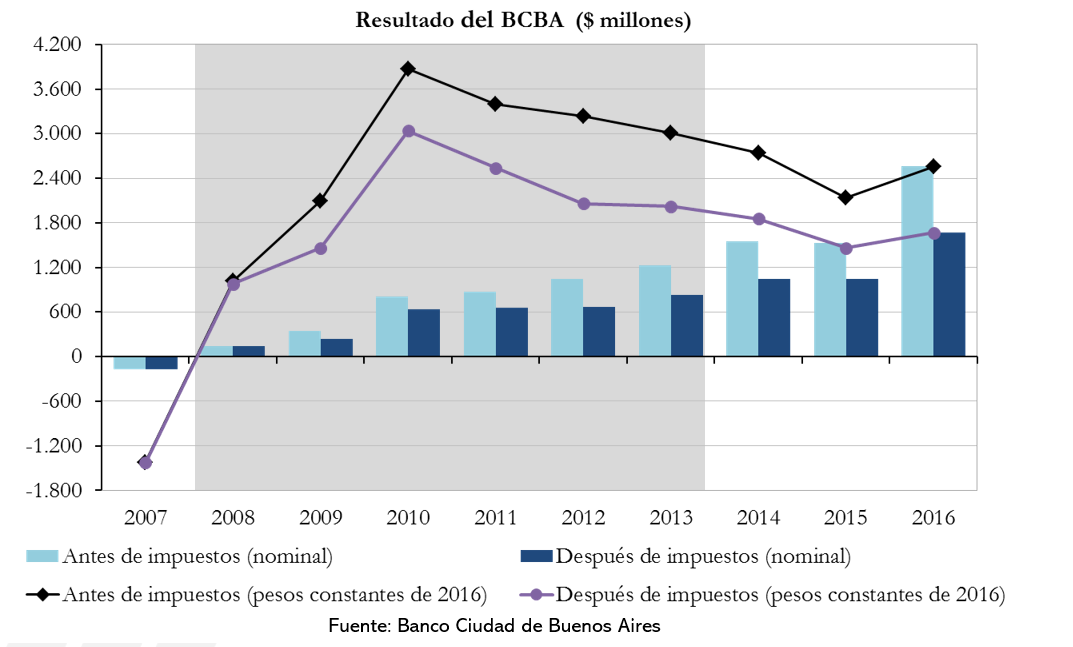
\includegraphics[width=12cm]{P3.png}\

%\end{frame}

%---------------------------------------------------------------------------%

%\begin{frame}{La Presidencia de Macri en dos tiempos. Tiempo I}

%\centering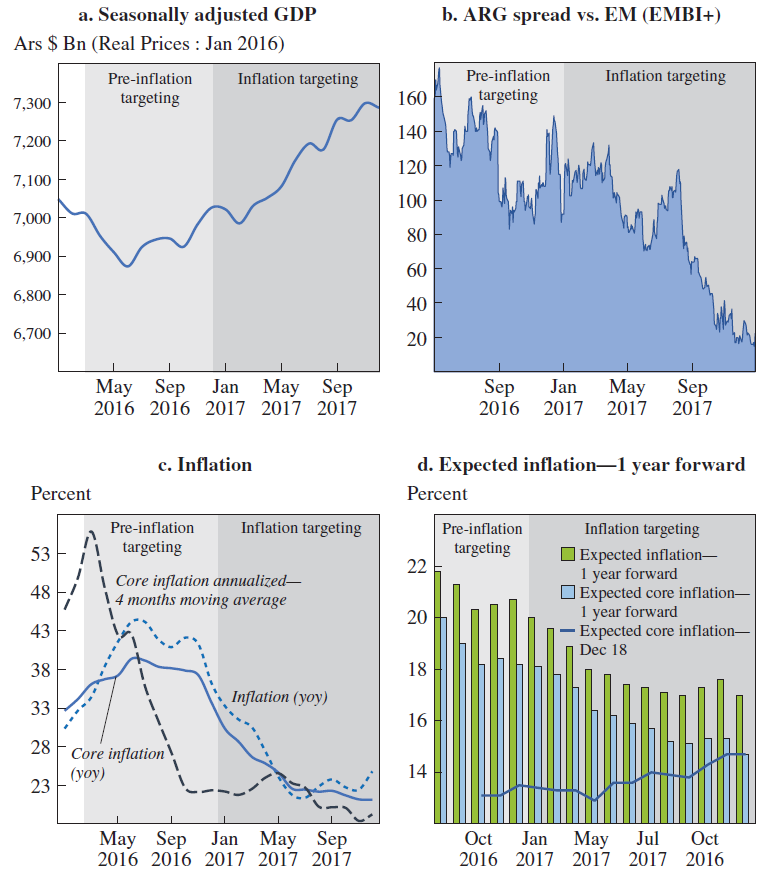
\includegraphics[width=7cm]{MM1.png}\

%end{frame}

%---------------------------------------------------------------------------%

%\begin{frame}{La Presidencia de Macri en dos tiempos. Tiempo II}

%\centering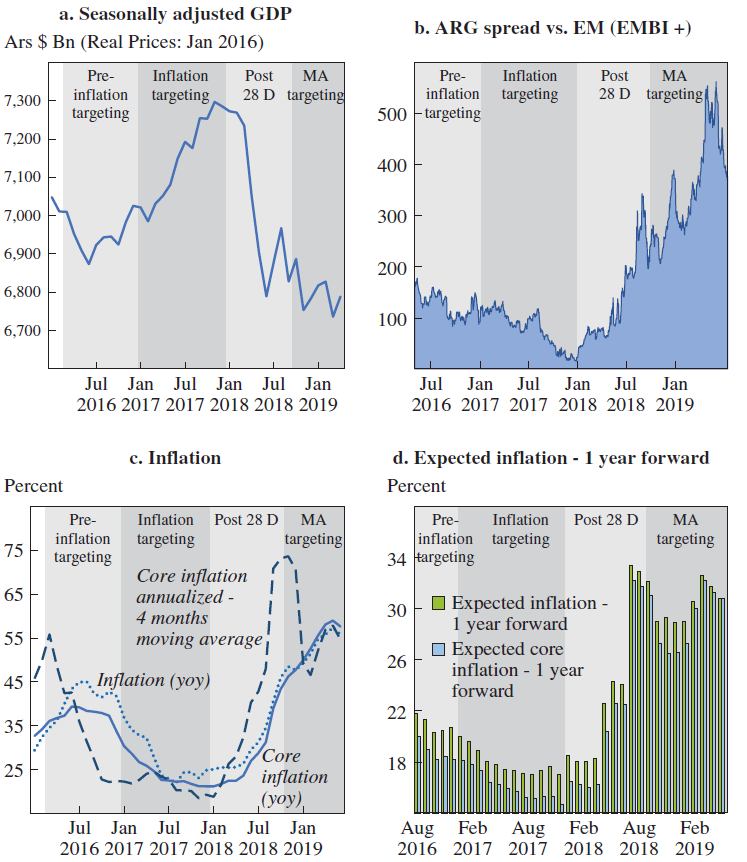
\includegraphics[width=7cm]{MM2.png}\

%\end{frame}

%---------------------------------------------------------------------------%

\begin{frame}{Mercados vs Planificacion}
    
    \begin{itemize}
        \item En la primera clase vimos el ejemplo de los tazones
        \item El ejemplo nos permite ilustrar los problemas y ventajas de la asignacion mercado vs planificacion
        \item La planificacion tiene tres problemas
        \begin{itemize}
            \item Genera incentivos incorrectos 
            \item Es muy intensivo en informacion requerida (necesita conocer preferencias y costos).
            \item Resulta inconsistente con las libertades politicas
            \item Concepto de "Libertad como desarrollo" de Amartya Sen. 
        \end{itemize}
    \end{itemize}
    
    
\end{frame}


\begin{frame}{Mercados vs Planificacion}
    
    \begin{itemize}
        \item Ejemplo de Cheqoslovaquia: fabricas que producían lo que no se demandaba
    \end{itemize}

\centering  
    \href{https://www.youtube.com/watch?v=u5hzmwGW4Ac}{
    
\includegraphics[scale=0.95]{images/Goodbyelenin.png}}  
    
\end{frame}



    


\begin{frame}{La mano invisible de Adam Smith}
    \begin{quote}
    “No es la benevolencia del carnicero, cervecero o panadero de donde obtendremos nuestra cena, sino de su preocupación por sus propios intereses”
\end{quote}
\end{frame}

\begin{frame}{La eficiencia de mercado en términos gráficos I}
    

\begin{figure} [H]
\centering
\begin{tikzpicture}[scale=0.6]
\draw[thick,<->] (0,10) node[above]{$P$}--(0,0)--(10,0) node[right]{$Q$};
\node [below left] at (0,0) {$0$};
\node [below] at (4.5,0) {$Q^*=100$};
\node [above] at (7/2,5.5) {$E$};
\node [left] at (0,5) {$P^*=30$};
%\node [left] at (0,6.85) {$40$};
\node [left] at (0,8.5) {$50$};
%\node [below] at (1.75,0) {50};
%\draw[semithick, red](1.75,5)--(1.75,6.85);
%\draw[thick,gray, dashed](1.75,0)--(1.75,6.85)--(0,6.85);
\draw[](0,5)--(7/2,5)--(7/2,0);
\draw[black, domain=0:7] plot (\x, {8.5-\x}) node[right] {$D$};
\draw[black, domain=0:7] plot (\x, {1.5+\x}) node[right] {$O$};
\end{tikzpicture}
\caption{\textbf{El equilibrio del mercado}}
\label{fig:16.1}
\end{figure} 

El mercado produce la cantidad optima del bien: solo se produce si vale m'as que lo que cuesta producirlo.


\end{frame}


\begin{frame}{La eficiencia de mercado en términos gráficos II}
    

\begin{figure}[H]
\tikzset{every picture/.style={line width=0.75pt}} %set default line width to 0.75pt        

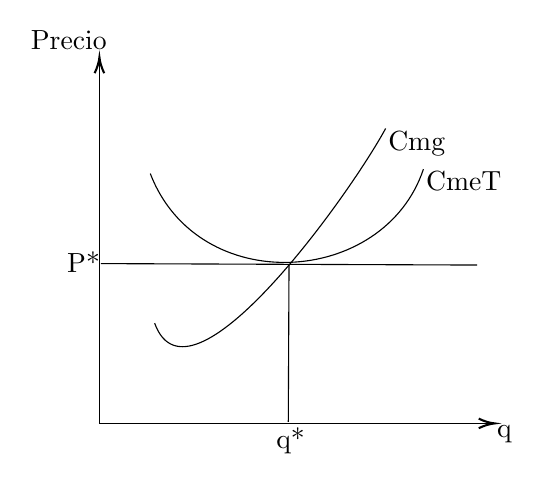
\begin{tikzpicture}[x=0.75pt,y=0.75pt,yscale=-0.7,xscale=0.7] 
%uncomment if require: \path (0,1657); %set diagram left start at 0, and has height of 1657

%Straight Lines [id:da6123979361342768] 
\draw    (74,298) -- (344,298) ;
\draw [shift={(346,298)}, rotate = 180] [color={rgb, 255:red, 0; green, 0; blue, 0 }  ][line width=0.75]    (10.93,-3.29) .. controls (6.95,-1.4) and (3.31,-0.3) .. (0,0) .. controls (3.31,0.3) and (6.95,1.4) .. (10.93,3.29)   ;
%Straight Lines [id:da5131707791527922] 
\draw    (74,298) -- (74,48) ;
\draw [shift={(74,46)}, rotate = 450] [color={rgb, 255:red, 0; green, 0; blue, 0 }  ][line width=0.75]    (10.93,-3.29) .. controls (6.95,-1.4) and (3.31,-0.3) .. (0,0) .. controls (3.31,0.3) and (6.95,1.4) .. (10.93,3.29)   ;
%Straight Lines [id:da6346804843028921] 
\draw    (75,188) -- (334,189) ;
%Curve Lines [id:da697350144213293] 
\draw    (109,126) .. controls (142,212) and (270,204) .. (297,123) ;
%Curve Lines [id:da9799910224345574] 
\draw    (112,229) .. controls (136,295) and (246,141) .. (271,95) ;
%Straight Lines [id:da5845279516726063] 
\draw    (204.5,188.5) -- (204,297) ;

% Text Node
\draw (25,26) node [anchor=north west][inner sep=0.75pt]   [align=left] {Precio};
% Text Node
\draw (346,298) node [anchor=north west][inner sep=0.75pt]   [align=left] {q};
% Text Node
\draw (297,123) node [anchor=north west][inner sep=0.75pt]   [align=left] {CmeT};
% Text Node
\draw (271,95) node [anchor=north west][inner sep=0.75pt]   [align=left] {Cmg};
% Text Node
\draw (50,178) node [anchor=north west][inner sep=0.75pt]   [align=left] {P*};
% Text Node
\draw (194,299) node [anchor=north west][inner sep=0.75pt]   [align=left] {q*};
\end{tikzpicture}
  \caption{El equilibrio de largo plazo de una empresa}
\end{figure}


El mercado produce cada bien al costo medio menor posible dada la tecnologia! 


\end{frame}


\begin{frame}{Distorsiones al equilibrio de mercado}
    \begin{itemize}
        \item En muchas ocasiones el mercado no funciona tan perfectamente. Las proximas clases son para analizar esos desvios.
        \item Hay dos tipos de desvios
        \begin{itemize}
            \item Los creados por el hombre
            \item Los que se imponen por caracteristicas de la realidad
        \end{itemize}
    \end{itemize}
\end{frame}


\begin{frame}{Distorsiones al equilibrio de mercado}
    \begin{itemize}
        \item Creadas por el hombre, 
        \begin{itemize}
            \item Monopolios artificiales (farmacias, escribanos, low cost)
            \item Impuestos
            \item Precios maximos o minimos (cepo)
            \item Regulacion (ley de alquileres)
        
        \end{itemize}
    \end{itemize}
\end{frame}

\begin{frame}{Distorsiones al equilibrio de mercado}
    \begin{itemize}
        \item Por las caracteristicas de la realidad 
        \begin{itemize}
            \item Monopolios naturales (red electrica)            \item Externalidades
            \item Problemas de informacion
            \begin{itemize}
                \item Informacion asimetrica
                \item Acciones ocultas (moral hazard)
            \end{itemize}
            \item Bienes publicos 
        
        \end{itemize}
    \end{itemize}
\end{frame}




\begin{frame}{Impuestos}




 \begin{figure} [H]
\caption{Costo de eficiencia de Impuestos}
   \centering
\begin{tikzpicture}[scale=0.6]
\draw[very thick,<->] (0,10) node[above]{$P$}--(0,0)--(10,0) node[right]{$Q$};
\draw[semithick](1,2)--(8,9) node[right]{$O'$};
\draw[semithick](2,1)--(9,8) node[right]{$O$};
\draw[semithick](1,9)--(9,1) node[right]{$D$};
 \path[pattern=horizontal lines,pattern color=black] (4.5,3.6)--(4.5,5.5)--(5.4,4.5);
\draw[semithick,dashed,gray](0,5.5)--(4.5,5.5)--(4.5,0);
\draw[semithick,dashed, gray](0,3.6)--(4.5,3.6);
\node [right] at (7,5) {\scriptsize Triángulo de};
\node [right] at (7.25,4.5) {\scriptsize Harberger};
\draw[semithick, <-] (5.3,4.2)..controls (5.8,3.8) and (6.8,3.8)..(7.5,4.2);
\draw[semithick,dashed,gray](0,4.5)--(5.5,4.5)--(5.5,0);
\node[below] at(5.5,0) {\footnotesize $Q_c$};
\node[below] at(4.5,0) {\footnotesize $Q'$};
\node[left] at(0,4.5) {\footnotesize $P_c$};
\node[left] at(0,5.5) {\footnotesize $P'_D$};
\node[left] at(0,3.6) {\footnotesize $P'_O$};
\end{tikzpicture}
\label{fig:19.1}
\end{figure}

\end{frame}

\begin{frame}{Minimizando las distorsiones}


\begin{figure} [H]
\caption{Impuestos con producto totalmente inelastico}
    \centering
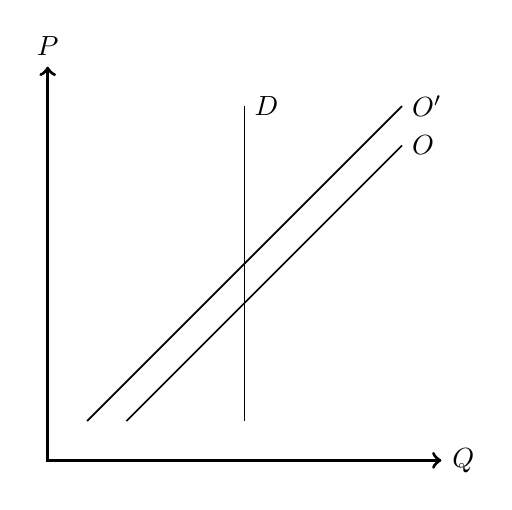
\begin{tikzpicture}[scale=0.5]
\draw[ very thick,<->] (0,10) node[above]{$P$}--(0,0)--(10,0) node[right]{$Q$};
%\node [below left] at (0,0) {$0$};
\draw[semithick](1,1)--(9,9) node[right]{$O'$};
\draw[semithick](2,1)--(9,8) node[right]{$O$};
\draw[semithick](5,1)--(5,9) node[right]{$D$};
\end{tikzpicture}
\label{fig:20.1}
\end{figure} 

\begin{itemize}
    \item Queremos grabar los bienes mas inelasticos
    \item Si todos los bienes tienen la misma elasticidad entonces misma tasa
\end{itemize}
\end{frame}

\begin{frame}{Incidencia de los impuestos}
    
\end{frame}


\begin{frame}{Precios Maximos}
    \begin{figure} [H]
\caption{Precio Máximo}
    \centering
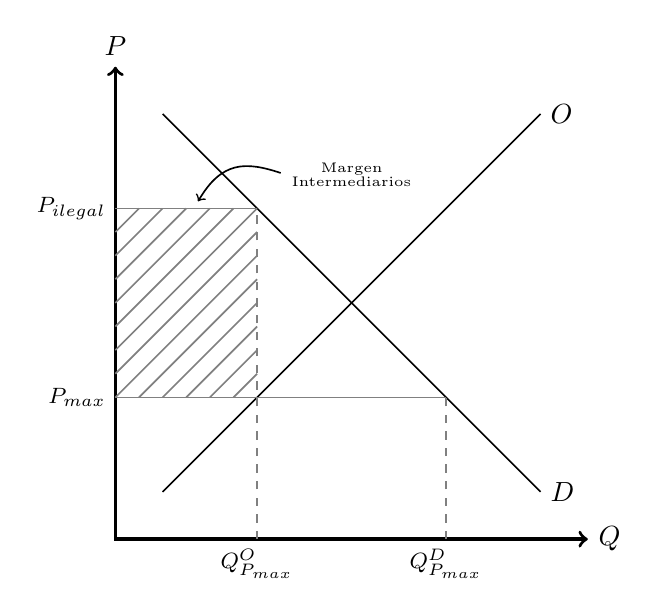
\begin{tikzpicture}[scale=0.6]
\draw[very thick,<->] (0,10) node[above]{$P$}--(0,0)--(10,0) node[right]{$Q$};
\draw[semithick](1,1)--(9,9) node[right]{$O$};
\draw [semithick] (1,9)--(9,1) node[right]{$D$};
\draw[semithick, gray] (0,6.5)--(0.5,7);
\draw[semithick, gray] (0,6)--(1,7);
\draw[semithick, gray] (0,5.5)--(1.5,7);
\draw[semithick, gray] (0,5)--(2,7);
\draw[semithick, gray] (0,4.5)--(2.5,7);
\draw[semithick, gray] (0,4)--(3,7);
\draw[semithick, gray] (0,3.5)--(3,6.5);
\draw[semithick, gray] (0,3)--(3,6);
\draw[semithick, gray] (0.5,3)--(3,5.5);
\draw[semithick, gray] (1,3)--(3,5);
\draw[semithick, gray] (1.5,3)--(3,4.5);
\draw[semithick, gray] (2,3)--(3,4);
\draw[semithick, gray] (2.5,3)--(3,3.5);
\draw[thick, gray, dashed](3,0)--(3,7) ;
\draw[semithick, gray](0,3)--(7,3);
\draw[thick, gray, dashed](7,0)--(7,3) ;
\draw[semithick, gray](0,7)--(3,7);
%\draw[semithick, gray,dashed](3,3)--(7.5,3);
\node[left] at (0,3){\footnotesize $P_{max}$};
\node[left] at (0,7){\footnotesize $P_{ilegal}$};
\node[below] at (3,0){\footnotesize $Q_{P_{max}}^{O}$};
\node[below] at (7,0){\footnotesize $Q_{P_{max}}^{D}$};
\draw[semithick, <-] (1.75,7.15).. controls (2.25,8) and (2.75,8).. (3.5,7.75);
\node[above] at (5,7.5) {\tiny Margen};
\node[above] at (5,7.25) {\tiny Intermediarios};
\end{tikzpicture}
\label{fig:20.2}
\end{figure}  
\end{frame}

\begin{frame}{Precio minimo sin mercado paralelo}

\begin{figure} [H]

    \centering
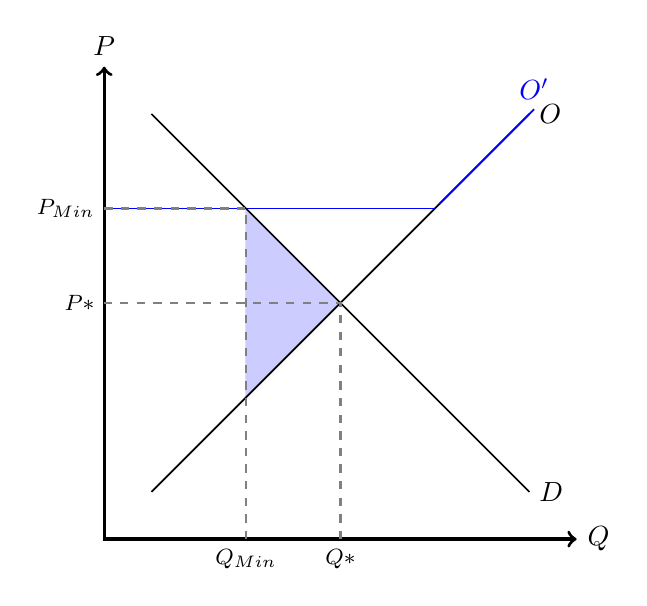
\begin{tikzpicture}[scale=0.6]
\draw[very thick,<->] (0,10) node[above]{$P$}--(0,0)--(10,0) node[right]{$Q$};
\draw[fill,blue!20] (5,5)--(3,7)--(3,3);
\draw [semithick](1,1)--(9,9) node[right]{$O$};
\draw [semithick, blue](7.1,7.1)--(9.1,9.1) node[above]{$O'$};
\draw [semithick, blue](7,7)--(0,7);
\draw [semithick](1,9)--(9,1) node[right]{$D$};
\draw[thick, gray, dashed](3,0)--(3,7) ;
\draw[thick, gray, dashed](0,7)--(3,7) ;
\draw[thick, gray, dashed](5,0)--(5,5)--(0,5) ;
%\node[left] at (0,3){\footnotesize $P^{'}_D$};
\node[left] at (0,7){\footnotesize $P_{Min}$};
\node[below] at (3,0){\footnotesize $Q_{Min}$};
\node[left] at (0,5){\footnotesize $P*$};
\node[below] at (5,0){\footnotesize $Q*$};
\end{tikzpicture}
\label{fig:20.7}
\end{figure} 

\end{frame}

 

\begin{frame}{Precio minimo con mercado paralelo}

\begin{figure} [H]

    \centering
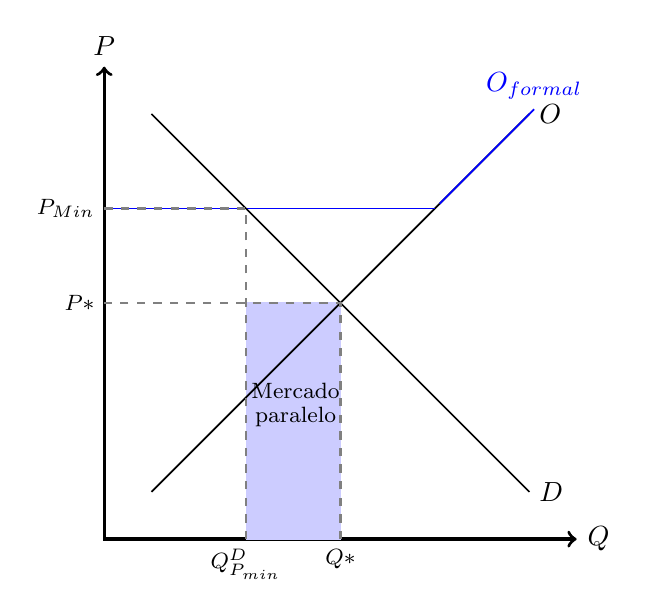
\begin{tikzpicture}[scale=0.6]
\draw[very thick,<->] (0,10) node[above]{$P$}--(0,0)--(10,0) node[right]{$Q$};
\draw[fill,blue!20]
(3,0)--(5,0)--(5,5)--(3,5);
\draw [semithick](1,1)--(9,9) node[right]{$O$};
\draw [semithick, blue](7.1,7.1)--(9.1,9.1) node[above]{$O_{formal}$};
\draw [semithick, blue](7,7)--(0,7);
\draw [semithick](1,9)--(9,1) node[right]{$D$};
\draw[thick, gray, dashed](3,0)--(3,7) ;
\draw[thick, gray, dashed](0,7)--(3,7) ;
%\draw[thick, gray, dashed](0,7)--(7,7)--(7,3)--(0,3) ;
\draw[thick, gray, dashed](5,0)--(5,5)--(0,5) ;
%\node[left] at (0,3){\footnotesize $P^{'}_D$};
\node[left] at (0,7){\footnotesize $P_{Min}$};
\node[below] at (3,0){\footnotesize $Q_{P_{min}}^{D}$};
\node[left] at (0,5){\footnotesize $P*$};
\node[below] at (5,0){\footnotesize $Q*$};
\node[below] at (4.05,3.5){\footnotesize Mercado};
\node[below] at (4.05,3){\footnotesize paralelo};
\end{tikzpicture}
\label{fig:20.7b}
\end{figure}  

\end{frame}








\begin{frame}{Precios sostén}
    \begin{figure} [H]
\caption{Pérdidas por la distorsión}
    \centering
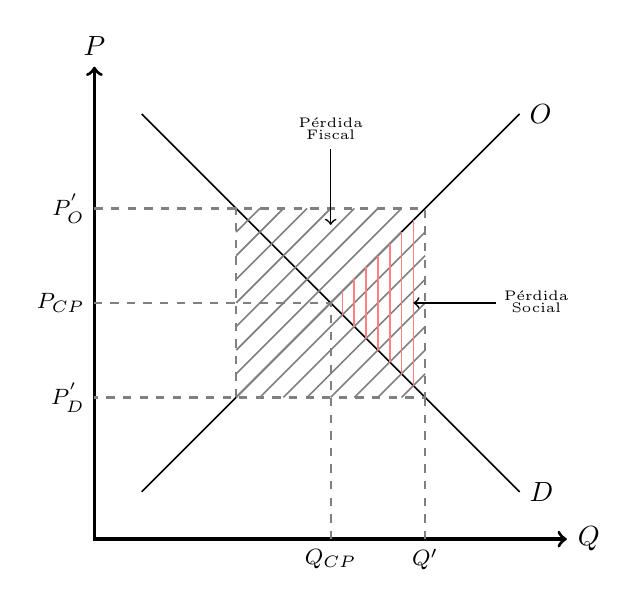
\begin{tikzpicture}[scale=0.6]
\draw[very thick,<->] (0,10) node[above]{$P$}--(0,0)--(10,0) node[right]{$Q$};
\draw [semithick](1,1)--(9,9) node[right]{$O$};
\draw [semithick](1,9)--(9,1) node[right]{$D$};
 \draw[semithick, gray] (3,6.5)--(3.5,7);
\draw[semithick, gray] (3,6)--(4,7);
\draw[semithick, gray] (3,5.5)--(4.5,7);
\draw[semithick, gray] (3,5)--(5,7);
\draw[semithick, gray] (3,4.5)--(5.5,7);
\draw[semithick, gray] (3,4)--(6,7);
\draw[semithick, gray] (3,3.5)--(6.5,7);
\draw[semithick, gray] (3,3)--(6.5,6.5);
\draw[semithick, gray] (3.5,3)--(7,6.5);
\draw[semithick, gray] (4,3)--(7,6);
\draw[semithick, gray] (4.5,3)--(7,5.5);
\draw[semithick, gray] (5,3)--(7,5);
\draw[semithick, gray] (5.5,3)--(7,4.5);
\draw[semithick, gray] (6,3)--(7,4);
\draw[semithick, gray] (6.5,3)--(7,3.5);
\draw[semithick, red!50] (6.75,3.25)--(6.75,6.75);
\draw[semithick, red!50] (6.5,3.5)--(6.5,6.5);
\draw[semithick, red!50] (6.25,3.75)--(6.25,6.25);
\draw[semithick, red!50] (6,4)--(6,6);
\draw[semithick, red!50] (5.75,4.25)--(5.75,5.75);
\draw[semithick, red!50] (5.5,4.5)--(5.5,5.5);
\draw[semithick, red!50] (5.25,4.75)--(5.25,5.25);
\draw[thick, gray, dashed](3,3)--(3,7) ;
\draw[thick, gray, dashed](7,0)--(7,3) ;
\draw[thick, gray, dashed](0,7)--(7,7)--(7,3)--(0,3) ;
\draw[thick, gray, dashed](5,0)--(5,5)--(0,5) ;
 \node[left] at (0,3){\footnotesize $P^{'}_D$};
 \node[left] at (0,7){\footnotesize $P^{'}_O$};
\node[below] at (7,0){\footnotesize $Q'$};
 \node[left] at (0,5){\footnotesize $P_{CP}$};
\node[below] at (5,0){\footnotesize $Q_{CP}$};
\draw[semithick, <-] (5,6.65)--(5,8.25);
\draw[semithick, ->] (8.5,5)--(6.75,5);
\node[above] at (5,8.5) {\tiny Pérdida};
\node[above] at (5,8.25) {\tiny Fiscal};
\node[above] at (9.35,4.85) {\tiny Pérdida};
\node[above] at (9.35,4.6) {\tiny Social};
\end{tikzpicture}
\label{fig:20.3}
\end{figure}  

\end{frame}


 
%\begin{frame}{El mercado de Berlin}
 %   \begin{figure}[htp]
%\href{https://twitter.com/andreaskluth/status/1366691926804754440} {\makebox[\textwidth][c]{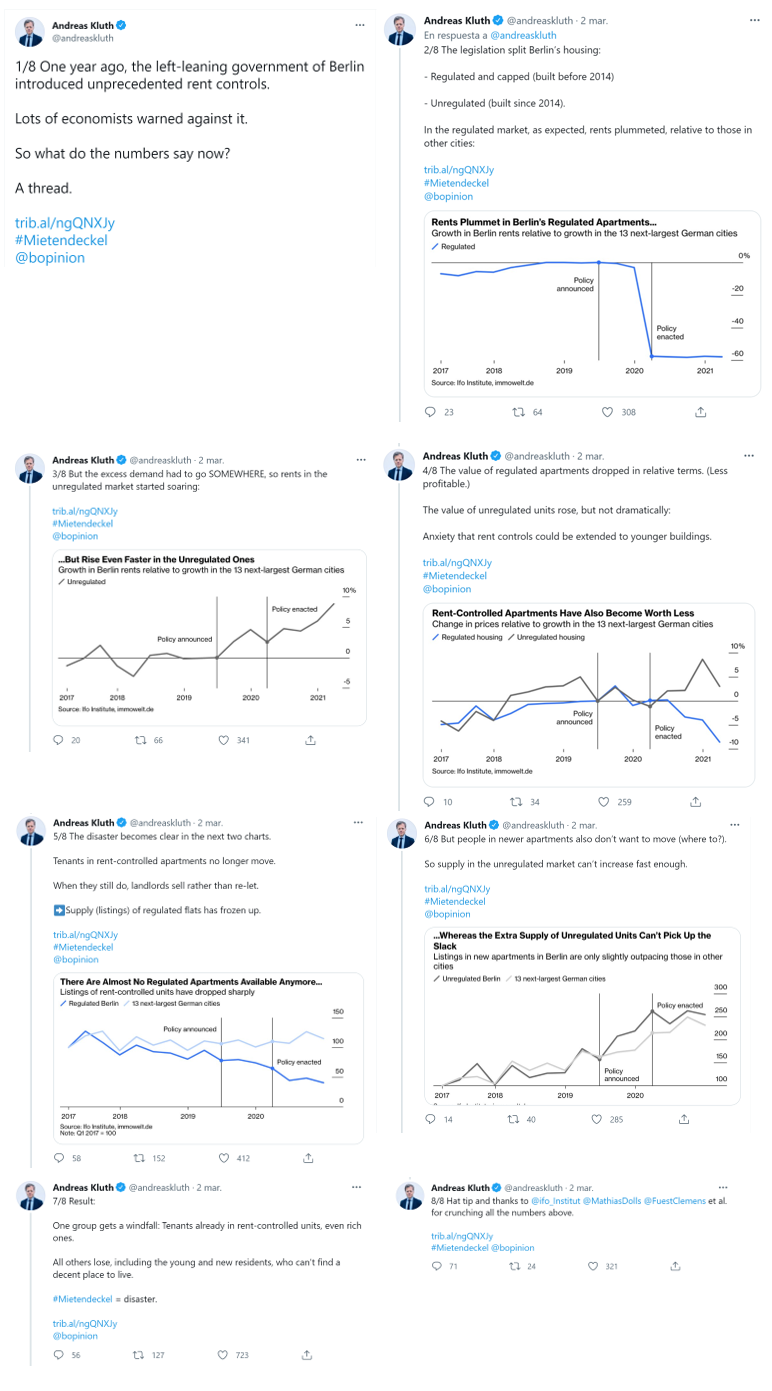
\includegraphics[width=0.45\textwidth]{images/TW.1.png}}} 
%\end{figure}
%Son muchos tweet en un imagen y para que entre todo queda muy chico. Igual haciendo click te lleva al hilo.
%\end{frame}



\begin{frame}{Distorsiones del Monopolio}
    \begin{figure} [H]
\caption{Precio Máximo en monopolio}
    \centering
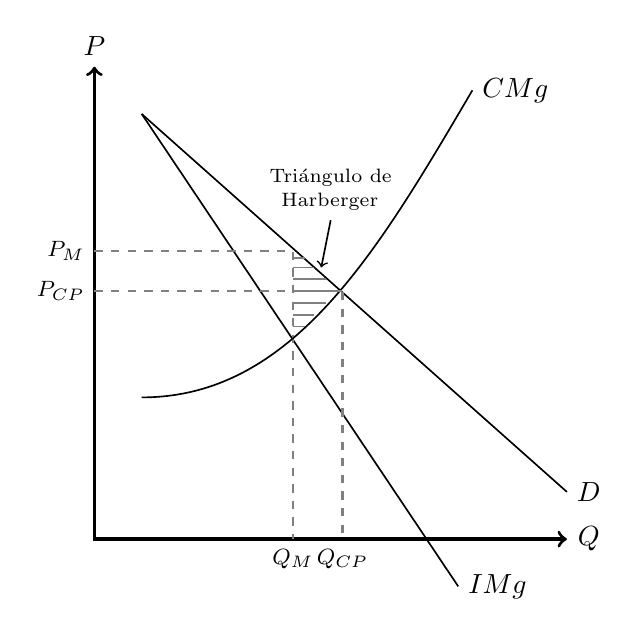
\begin{tikzpicture}[scale=0.6]
\draw[very thick,<->] (0,10) node[above]{$P$}--(0,0)--(10,0) node[right]{$Q$};
\draw[semithick](1,9)--(10,1) node[right]{$D$};
\draw[semithick](1,9)--(7.7,-1) node[right]{$IMg$};
\draw[thick,dashed,gray](0,6.1)--(4.2,6.1)--(4.2,0);
\draw[thick,dashed,gray](0,5.25)--(5.25,5.25)--(5.25,0);
%\draw(1,1)--(9,9);
\draw[semithick](1,3).. controls (4.2,3) and (6,6.1)..(8,9.5) node[right]{$CMg$};
\draw[semithick, gray] (4.2,5.95) to (4.45,5.95) ;
\draw[semithick, gray] (4.2,5.75) to (4.65,5.75) ;
\draw[semithick, gray] (4.2,5.5) to (4.9,5.5) ;
\draw[semithick, gray] (4.2,5.25) to (5.25,5.25) ;
\draw[semithick, gray] (4.2,5) to (4.9,5) ;
\draw[semithick, gray] (4.2,4.75) to (4.65,4.75) ;
\draw[semithick, gray] (4.2,4.5) to (4.45,4.5) ;
 \node [right] at (3.5,7.65) {\scriptsize Triángulo de};
 \node [right] at (3.75,7.15) {\scriptsize Harberger};
\draw[semithick, <-] (4.8,5.75)--(5,6.75);
\node[below] at(4.2,0) {\footnotesize $Q_M$};
\node[below] at(5.25,0) {\footnotesize $Q_{CP}$};
\node[left] at(0,6.1) {\footnotesize $P_{M}$};
\node[left] at(0,5.25) {\footnotesize $P_{CP}$};
\end{tikzpicture}
\label{fig:20.4}
\end{figure}
\end{frame}

  \begin{frame}{Como regular un monopolio}
    \begin{itemize}
        \item Lo primero que hay que hacer es entender porque hay un monopolio
        \item Y tratar de eliminarlo
        \item Alcanza con decir que una empresa es grande para definir un monopolio? 
        \item No! ... si los mercados son contestables.
        \item Solo en casos extremos debieramos apelar a la regulacion de precios.
    \end{itemize}
\end{frame}

\begin{frame}{Como regular un monopolio}
    \begin{figure} [H]
\caption{Monopolio regulado}
    \centering
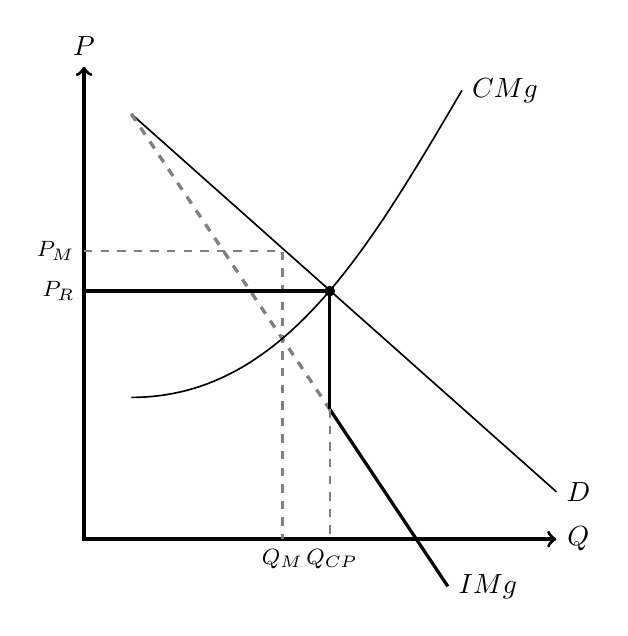
\begin{tikzpicture}[scale=0.6]
\draw[very thick,<->] (0,10) node[above]{$P$}--(0,0)--(10,0) node[right]{$Q$};
\draw[semithick](1,9)--(10,1) node[right]{$D$};
%\draw[semithick](1,9)--(7.7,-1) node[right]{$IMg$};
\draw[very thick,dashed,gray](1,9)--(5.2,2.75);
\draw[very thick](5.2,2.75)--(7.7,-1) node[right]{$IMg$};
\draw[thick,dashed,gray](5.2,2.75)--(5.2,0);
\draw[thick,dashed,gray](0,6.1)--(4.2,6.1)--(4.2,0);
\draw[very thick](0,5.25)--(5.2,5.25)--(5.2,2.75);
%\draw(1,1)--(9,9);
\draw[semithick](1,3).. controls (4.2,3) and (6,6.1)..(8,9.5) node[right]{$CMg$};
\node[below] at(4.2,0) {\footnotesize $Q_M$};
\node[below] at(5.25,0) {\footnotesize $Q_{CP}$};
\node[left] at(0,6.1) {\footnotesize $P_{M}$};
\node[left] at(0,5.25) {\footnotesize $P_{R}$};
\draw[fill](5.2,5.25) circle [radius =0.1];
    \end{tikzpicture}
\label{fig:20.5}
\end{figure} 

\end{frame}


\begin{frame}{Monopolio Natural}
    \begin{figure} [H]
\caption{Monopolio Natural}
    \centering
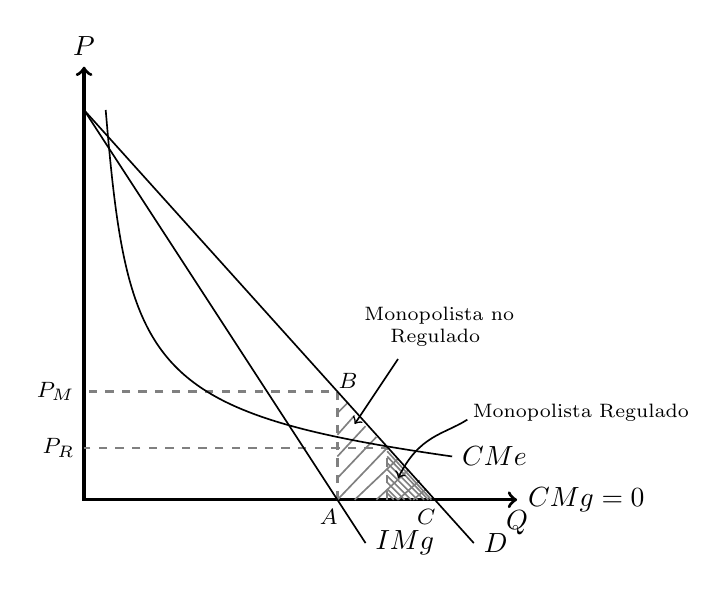
\begin{tikzpicture}[scale=0.55]
\draw[very thick,<->] (0,10) node[above]{$P$}--(0,0)--(10,0) node[right]{$CMg=0$} node[below]{$Q$};
\draw[semithick, gray] (5.85,2)--(6.1,2.25);
\draw[semithick, gray] (5.85,1.5)--(6.25,1.95);
\draw[semithick, gray] (5.85,1)--(6.5,1.7);
\draw[semithick, gray] (5.85,0.5)--(6.75,1.45);
\draw[semithick, gray] (5.85,0)--(7,1.2);
\draw[semithick, gray] (6.25,0)--(7.25,0.95);
\draw[semithick, gray] (6.75,0)--(7.5,0.7);
\draw[semithick, gray] (7.25,0)--(7.75,0.45);
\draw[semithick, gray] (7.6,0)--(7.9,0.25);
\draw[semithick, gray] (7,0.15  )--(7.15,0);
\draw[semithick, gray] (7,0.25)--(7.25,0);
\draw[semithick, gray] (7,0.4)--(7.4,0);
\draw[semithick, gray] (7,0.55)--(7.55,0);
\draw[semithick, gray] (7,0.7)--(7.7,0);
\draw[semithick, gray] (7,0.85)--(7.85,0);
\draw[semithick, gray] (7,1)--(7.95,0);
\draw[semithick, gray] (7,1.12)--(8.02,0);
\draw[thick, dashed,gray] (5.85,0)--(5.85,2.5)--(0,2.5);
\draw[thick, dashed,gray] (7,0)--(7,1.2)--(0,1.2);
\node[left] at (0,2.5) {\footnotesize $P_M$};
\node[left] at (0,1.2) {\footnotesize $P_R$};
\node[below] at (5.65,0) {\footnotesize $A$};
\node[right] at (5.65,2.75) {\footnotesize $B$};
\node[below] at (7.9,0) {\footnotesize $C$};
\draw[semithick](0,9)--(9,-1) node[right]{$D$};
\draw[semithick](0,9)--(6.5,-1) node[right]{$IMg$};
\draw[semithick](0.5,9) ..controls (1,3) and (1.5,2) .. (8.5,1) node[right]{$CMe$};
\draw[semithick, <-] (6.25,1.75)--(7.25,3.25);
 \node [right] at (6.25,4.25) {\scriptsize Monopolista no};
 \node [right] at (6.85,3.75) {\scriptsize Regulado};
  \draw[semithick, <-] (7.25,0.5).. controls (7.75,1.5) and (8.3,1.5) ..(8.85,1.85);
   \node [right] at (8.75,2) {\scriptsize Monopolista Regulado};
\end{tikzpicture}
\label{fig:20.6}
\end{figure} 
\end{frame}


\begin{frame}{Poniéndole precio a una carretera  I}
     \begin{figure} [h!]
    \centering
    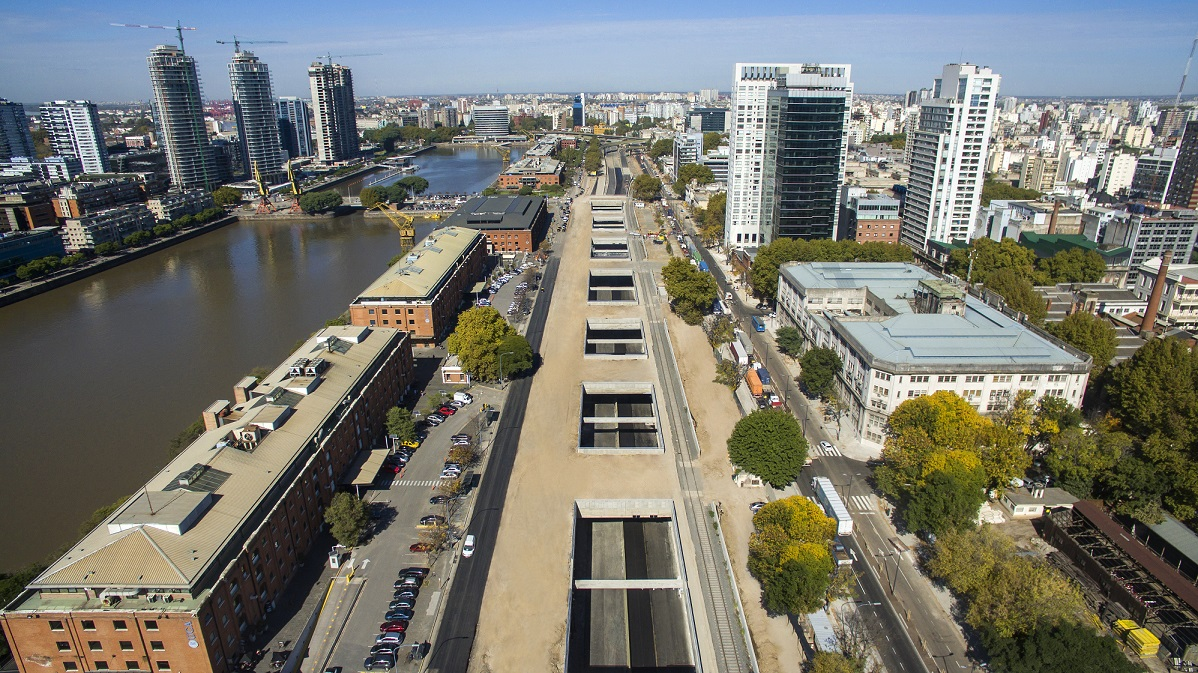
\includegraphics[width=0.80\textwidth]{images/Paseobajo.jpg}
    \caption{Paseo del bajo}
    \label{fig:}
\end{figure}
 
\end{frame}



\begin{frame}{Poniéndole precio a una carretera  II}
    \begin{figure} [H]
\centering
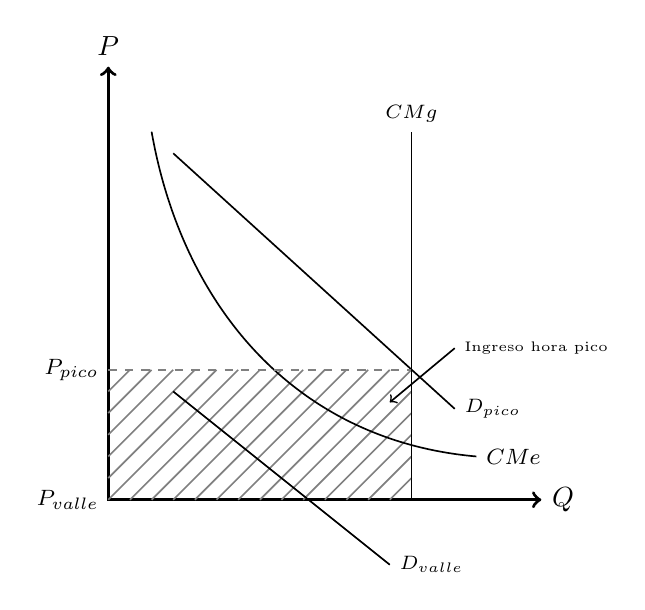
\begin{tikzpicture}[scale=0.55]
\draw[very thick,<->] (0,10) node[above]{$P$}--(0,0)--(10,0) node[right]{$Q$};
\draw[semithick, gray] (0,2.5)--(0.5,3);
\draw[semithick, gray] (0,2)--(1,3);
\draw[semithick, gray] (0,1.5)--(1.5,3);
\draw[semithick, gray] (0,1)--(2,3);
\draw[semithick, gray] (0,0.5)--(2.5,3);
\draw[semithick, gray] (0,0)--(3,3);
\draw[semithick, gray] (0.5,0)--(3.5,3);
\draw[semithick, gray] (1,0)--(4,3);
\draw[semithick, gray] (1.5,0)--(4.5,3);
\draw[semithick, gray] (2,0)--(5,3);
\draw[semithick, gray] (2.5,0)--(5.5,3);
\draw[semithick, gray] (3,0)--(6,3);
\draw[semithick, gray] (3.5,0)--(6.5,3);
\draw[semithick, gray] (4,0)--(7,3);
\draw[semithick, gray] (4.5,0)--(7,2.5);
\draw[semithick, gray] (5,0)--(7,2);
\draw[semithick, gray] (5.5,0)--(7,1.5);
\draw[semithick, gray] (6,0)--(7,1);
\draw[semithick, gray] (6.5,0)--(7,0.5);
\draw [semithick] (1,8.5) to [out=280,in=175] (8.5,1)node [right] {\footnotesize $CMe$};
\draw [semithick] (7,0) to (7,8.5);
\node[above] at (7,8.5) {\scriptsize $CMg$};
\draw [semithick] (8,2.1) node [right]  {\scriptsize$D_{pico}$} to (1.5,8);
\draw [semithick] (6.5,-1.5) node [right]  {\scriptsize$D_{valle}$} to (1.5,2.5);
\draw[thick, gray, dashed](0,3)--(7,3) ;
\node[left] at (0,3){\footnotesize $P_{pico}$};
\node[left] at (0,0){\footnotesize $P_{valle}$};
\draw[semithick, ->] (8,3.5)--(6.5,2.25);
\node[right] at (8,3.5) {\tiny Ingreso hora pico};
\end{tikzpicture}
\label{fig:20.7}
\end{figure} 
 
\end{frame}

 
\begin{frame}{Externalidades}
    \begin{itemize}
        \item Sucede cuando una decision economica genera un beneficio o costo no pecuniario
        \item Externalidades negativas: contaminacion
        \item Externalidades positivas: abejas y naranjos
    \end{itemize}
\end{frame}


\begin{frame}{Un ejemplo}
    \begin{itemize}
        \item Dos productores: una curtiembre y pescadores
        \item La producción de curtiembres genera contaminación que afecta la cantidad de peces en el rio
    \end{itemize}
\end{frame}

\begin{frame}{Una imagen}
    

 \begin{figure} [h!]
    \centering
    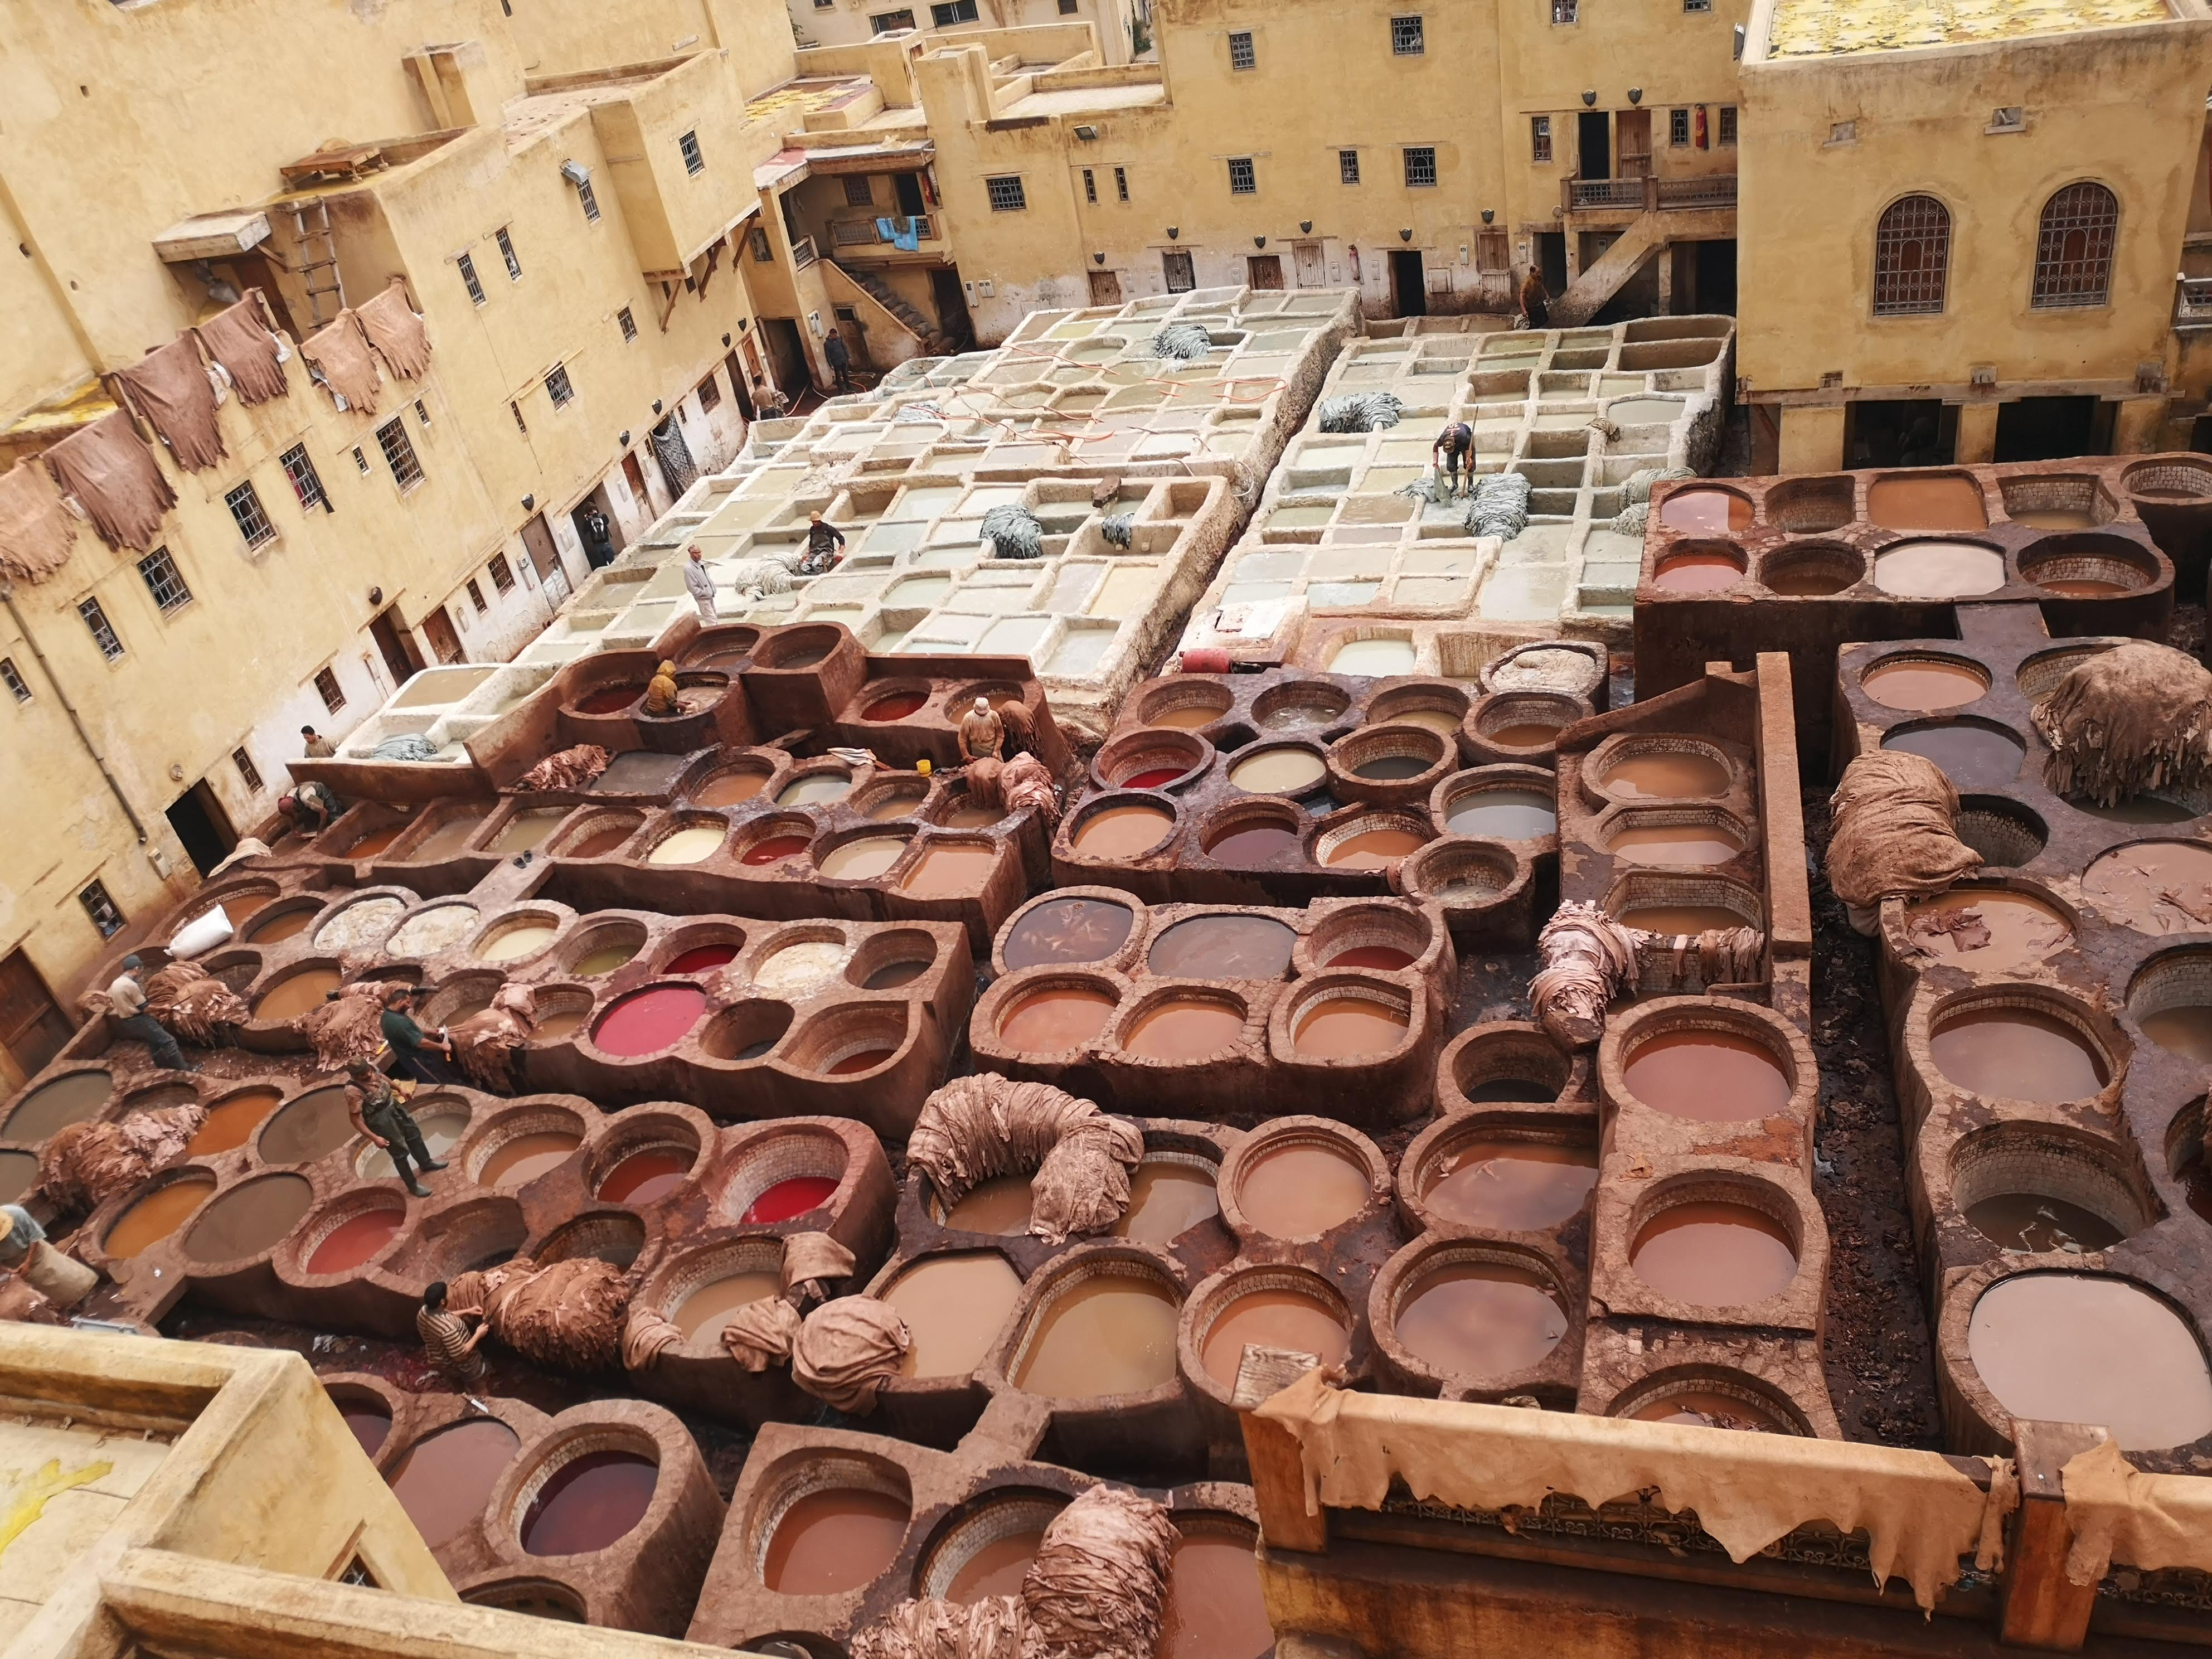
\includegraphics[width=0.8\textwidth]{images/Fez.jpg}
    \caption{Curtiembre en Fez}
    \label{fig:}
\end{figure}

\end{frame}


\begin{frame}{Como se suman los costos}
    \begin{figure} [H]
\centering
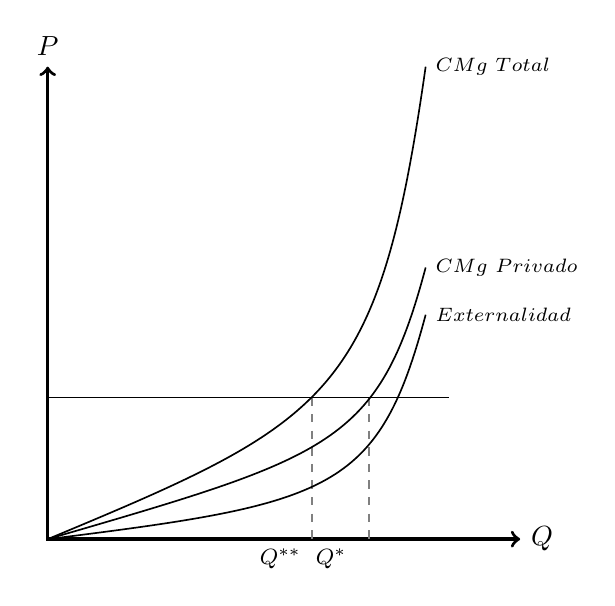
\begin{tikzpicture}[scale=0.6]
\draw[very thick,<->] (0,10) node[above]{$P$}--(0,0)--(10,0) node[right]{$Q$};
\draw[thick, dashed, gray] (5.6,3)--(5.6,0);
\draw[thick, dashed, gray] (6.8,3)--(6.8,0);
\draw [semithick] (0,0)..controls (6,1.75) and (7,2) .. (8,5.75) node [right] {\scriptsize $CMg \hspace{0.1cm} Privado$};
\draw [semithick] (0 ,0)..controls (6,0.75) and (7,1) .. (8,4.75) node [right] {\scriptsize $Externalidad$};
\draw [semithick] (0,0)..controls (6,2.5) and (7,3) .. (8,10) node [right] {\scriptsize $CMg \hspace{0.1cm} Total$};
\draw[semithick] (0,3)--(8.5,3);
\node[below] at (6,0) {\footnotesize $Q^{*}$};
\node[below] at (4.925,0) {\footnotesize $Q^{**}$};
\end{tikzpicture}
\caption{Externalidad}
\label{fig:21.1}
\end{figure} 

\end{frame}
 

\begin{frame}{Como corregir una externalidad}
    \begin{itemize}
        \item Una manera es regular la producción o el uso del contaminante
        \item La otra es gravar la actividad contaminante
    \end{itemize}
\end{frame}
  
\begin{frame}{Teorema de Coase}
    \begin{itemize}
        \item Coase dice que las externalidades no son un problema
        \item .... si los derechos de propiedad están bien definidos
        \item Esto es así porque "hay una ganancia para apropiar" de buscar un óptimo 
    \end{itemize}
\end{frame}


\begin{frame}{Coase I}
    \begin{figure} [H]
\centering
\begin{tikzpicture}[scale=0.6]
\draw[thick,<->] (0,10) node[above]{$P$}--(0,0)--(10,0) node[right]{$Q$};
\draw[fill,blue!15] (6.1,3.3)--(6.1,5)--(7.45,7.4)--(7.45,5)--(6.8,4);
% \draw[lines] (6.1,3.3)--(6.1,5)--(7.45,5)--(6.8,4);
% \draw[pattern=north west lines, pattern color=gray,solid] (6.1,3.3)--(6.1,5)--(7.45,5);
\path[pattern=horizontal lines,pattern color=black] (6.1,3.3)--(6.1,5)--(7.45,5);
\draw[thick, gray,dashed] (7.45,0)--(7.45,7.5);
\draw[thick, gray,dashed] (6.1,0)--(6.1,5);
\draw [semithick] (0,5) to (9,5) ;
\draw[semithick] (1,2)..controls (3,2) and (6,3) .. (8,9);
\draw[semithick] (1,1)..controls (3,1) and (7,2) .. (9,8.5);
\node[left] at (0,5) {\footnotesize $P^{*}$};
\node[below] at (7.45,0) {\footnotesize $Q^{*}$};
\node[below] at (6.1,0) {\footnotesize $Q^{**}$};
  \draw[semithick, <-] (6.75,4).. controls (7.15,3.75) and (7.7,3.75) ..(8.5,4);
   \node [right] at (8.9,4.15) {\scriptsize Pérdida};
   \node [right] at (8.5,3.75) {\scriptsize Curtiembres};
     \draw[semithick, <-] (6.85,5.8)--(5.75,7);
        \node [right] at (3.75,7.75) {\scriptsize Pérdida Total};
   \node [right] at (4.1,7.35) {\scriptsize Pescadores};
\end{tikzpicture}
\caption{Externalidad negativa}
\label{fig:21.2}
\end{figure} 
\end{frame}
 

\begin{frame}{Coase II}
    \begin{figure} [H]
\centering
\begin{tikzpicture}[scale=0.6]
\draw[thick,<->] (0,10) node[above]{$P$}--(0,0)--(10,0) node[right]{$Q$};
\draw[fill,blue!15] (0.05,1.05)--(0.05,3)--(4.05,3)--(4.05,1.8)--(2,1.14)--(1,1.05);
\path[pattern=vertical lines,pattern color=black] (0,1)--(0,2)--(1.5,2)--(3,2.4)--(4.05,3)--(4.05,1.8)--(3,1.45)--(1.5,1.1);
\draw[thick, gray,dashed] (4.05,0)--(4.05,3);
\draw [semithick] (0,3) to (9,3) ;
\draw[semithick] (0.25,2)..controls (3,2) and (6,3) .. (8,9);
\draw[semithick] (0.25,1)..controls (3,1) and (7,2) .. (9,8.5);
\node[left] at (0,3) {\footnotesize $P^{*}$};
\node[below] at (4.05,0) {\footnotesize $Q^{**}$};
\draw[semithick, ->] (-0.5,1.5)--(0.5,1.5);
\draw[semithick, <-] (1.5,2.65)--(1.5,3.75);   
\node [right] at (0.5,4.5) {\scriptsize Ganancia };
   \node [right] at (0.25,4.1) {\scriptsize Curtiembres};
         \node [right] at (-3,1.75) {\scriptsize Pérdida };
   \node [right] at (-3.25,1.35) {\scriptsize Pescadores};
\end{tikzpicture}
\caption{Externalidad negativa}
\label{fig:21.3}
\end{figure} 
\end{frame}


\begin{frame}{Bienes Públicos}
\begin{itemize}
    \item Vamos a distinguir los bienes por dos caracteristicas
    \begin{itemize}
        \item Si su consumo es rival
        \item Si su consumo es excluible
    \end{itemize}
\end{itemize}

\end{frame}



\begin{frame}{Bienes Públicos}
\begin{figure} [H]   
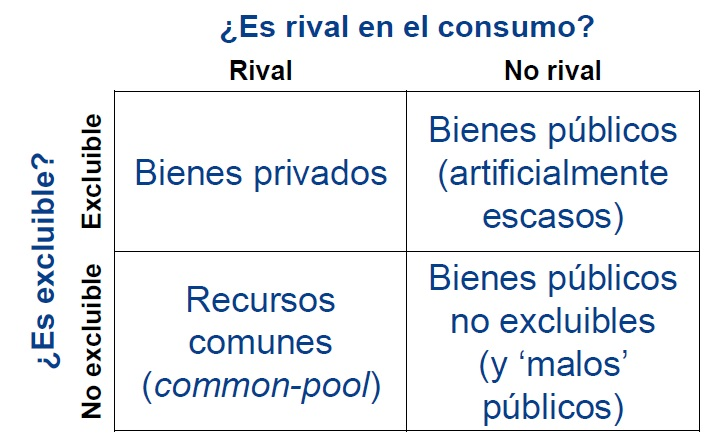
\includegraphics[scale=0.55]{images/C15.1.jpg}

\label{fig:15.1}
\end{figure}


\end{frame}


    
    
    \begin{frame}{Asimetrías de información}
        \begin{itemize}
            \item \textbf{1.Riesgo moral o acción oculta} alguien no puede ver las acciones del otro. 
    
\begin{figure} [H]   
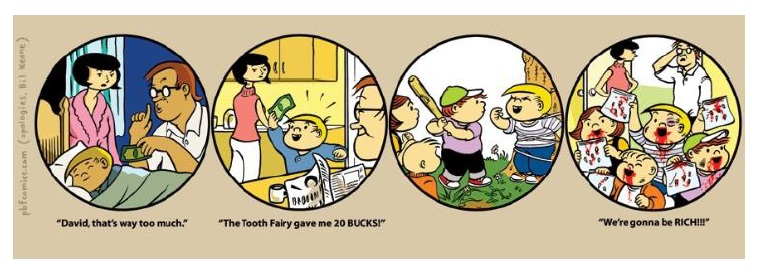
\includegraphics[scale=0.3]{images/C14.1.jpg}
\label{fig:14.1}
\end{figure}

\item Ejemplos: seguros en general, incentivos a ahorrar, etc. 

  \item \textbf{2 Atributos ocultos.} Es cuando no conocemos una característica de la contraparte. 
  
  \item Ejemplos: seguros en general, usados. 
  
  \item Ambos producen el problema de selección adversa, que quiere decir que solo vienen al mercado los clientes “malos” 
  \item El resultado es que el mercado incluso puede desaparecer!


        \end{itemize}
    \end{frame}
    
 
\begin{frame}{El mercado de los limones de Akerlof}
    

 


\begin{itemize}
    \item Dos tipos de autos: buenos y fallados
    \item q son buenos y (1-q) son malos 
\item Para el vendedor el auto bueno vale 1000 y el lemon 500. 
\item Para el comprador el auto bueno vale 1500 y el lemon 750. 

\item Vamos a ver cuanto estaría dispuesto a pagar un comprador y dado eso después vemos que le conviene hacer al vendedor. 

\item El comprador esta dispuesta a pagar seria su valor esperado. 

\item Si piensa que la probabilidad que un auto sea bueno sea  $\mu$ y que sea malo  $(1-\mu)$ el valor esperado para un auto típico en el mercado sería  $\mu 1500 + (1-\mu) 750= 750 + \mu 750$ 
\item El vendedor venderá un auto si lo que cobra por él supera lo que el lo valúa. 
\end{itemize}
\end{frame}

\begin{frame}{El mercado de los limones II}
    
\begin{itemize}
\item Si tiene un lemon lo venderá si 

\begin{equation}
    500 \leq 750 + \mu 750
\end{equation}

\item Que se da siempre. Lo cual quiere decir que si el vendedor tiene un lemon lo pone en el mercado siempre.

\item Si tiene un auto bueno, lo venderá si 
\begin{equation}
    1000 \leq 750 + \mu 750 \label{akerlof}
\end{equation}

\item Esto solo se daría si $\mu \geq \frac{1}{3}$. 
\end{itemize}
\end{frame}

\begin{frame}{El mercado de los limones III}
\begin{itemize}
\item  Si $ q \geq \frac{1}{3}$, (hay suficiente buenos) hay un equilibrio donde $\mu = q \geq \frac{1}{3}$ y $p= 750 + \mu 750$ y se venden los dos tipos de autos. 

\item Pero si $q \leq \frac{1}{3}$ entonces por la ecuación (\ref{akerlof}) sabemos que $\mu=0 $, lo cual quiere decir que se venden solo limones y el precio de venta es de $p= 750$. 


\item El mercado para autos buenos desapareció aun cuando dijimos al principio que estos tenían más valor para los consumidores que para los vendedores. ¡La mano invisible de Adam Smith no pudo operar por la asimetría de información!

\end{itemize} 
\end{frame}

\begin{frame}{Riesgo moral y el colapso del mercado de seguros}
 \begin{itemize}
     \item Un individuo que tiene que comprar un seguro de incendio para su casa. 
     \item Pueden pasar dos cosas. O que la casa no se incendie (llamemos a este evento B, por bueno) o que la casa se incendie (llamemos a este evento M por malo). 

\item B sucede con probabilidad $p$ y el evento malo con probabilidad $(1-p)$. 
\item Si se produce el evento malo, el individuo sufre una perdida de tamaño $L$.

\item La la probabilidad del evento bueno depende en parte de alguna acción del individuo, $p(e)$.

\item Quien ofrece el seguro no puede ver esta acción. 
\end{itemize}
\end{frame}

\begin{frame}{Riesgo moral II}
\begin{itemize}
\item Veamos que pasa si la compañía ofrece una cobertura de valor $C$ a un precio $\pi$. 

\item Si pasa el escenario bueno la utilidad para el individuo es 

\begin{equation}
    Y_B = y - \pi C
\end{equation}

\item Si se produce el evento malo su utilidad es 
\begin{equation}
    Y_M = y - L - \pi C + C
\end{equation}

\item ¿Qué $\pi$ podrían cobrar la compañía de seguros? Vamos a asumir el caso más favorable al asegurador, que es que la compañías de seguro salen hechas. 

\item La ecuación de ganancias de las aseguradoras es  
\begin{equation}
    \pi C - (1-p) C.
    \end{equation}

\item Si esta ganancia la hacemos $0$ el (menor) precio que puede cobrar la compañía es $\pi=(1-p)$.
\end{itemize}
\end{frame}

\begin{frame}{Riesgo moral III}
\begin{itemize}
\item Si el individuo compra una cobertura de $C=L$ en el evento bueno su utilidad es $y-\pi L$ y en el evento malo es $y-L-\pi L+L=y-\pi L $. 

\item Al comprar cobertura total, le es indiferente si se produce el evento bueno o el malo. 

\item Pero entonces $e=0$ y la probabilidad del siniestro va a ser más alta. 

\itiem Consideremos el caso en el cual si el individuo no hace nada el siniestro ocurre con probabilidad 1. En ese caso $p=0$ y $\pi=1$. 

\item La utilidad para el individuo de comprar seguro es $y-L$, que resulta peor que no comprar seguro. 

\item ¡Es decir que el mercado asegurador desaparece! 

  \end{itemize}   
\end{frame}


\begin{frame}{Discusión}
    \begin{itemize}
        \item Por que pierden valor los autos al salir de la concesionaria?
        \item Políticas de deducibles
        \item Obama care
    \end{itemize}
\end{frame}

%\begin{frame}{Teoría de los contratos}
%    \begin{itemize}
%        \item Dijimos que los economistas trabajan para mejorar la asignación
  %      \item Muchas veces para eso hay que tener "buenas reglas de juego"
  %      \item Los contratos establecen las reglas de juego de ciertas interacciones. 
  %      \item Libertad para definir un contrato - Ejecución del contrato
  %      \item En esta clase vamos a aprender a hacer un contrato
  %      \item Para ello vamos a analizar el problema del principal-agente
  %  \end{itemize}
%\end{frame}


%\begin{frame}{El problema del principal-agente}
%    \begin{itemize}
%        \item El Principal contrata a alguien para hacer algo
%        \item El Agente es la persona contratada para hacer la tarea
%        \item El agente toma decisiones que afectan al principal, pero
%esta motivado a seguir su propio interés - P.ej., votantes-políticos, empleador-empleado, accionista-CEO, pacientes-médicos, etc.
%        \item Usualmente el problema de P-A surge debido a asimetrías
%de información:
%\begin{itemize}
%    \item Es costoso para el principal ver lo que el agente hace
%    \item El agente sabe algo que el principal no
% \item Lo útil para el principal es costoso para el agente
%\end{itemize}
%\item Este es el problema que el contrato tiene que resolver.
%   \end{itemize}
%\end{frame}

%\begin{frame}{El problema del principal-agente II}
%    \begin{itemize}
%        \item Empleador y empleado
%        \begin{itemize}
%            \item El empleador contrata a un trabajo y le ofrece un
%contrato
%\item El empleado se esfuerza o no (no visible)
%\item Empleador le paga en función de lo producido

%        \end{itemize}
        
%\item Seguros del auto
%    \begin{itemize}
%            \item La compañía de seguro ofrece una póliza con deducibles
%            \item El conductor luego elije como manejar
%            \item La compañía paga los accidentes
%        \end{itemize}
        
%\item  Accionistas y su CEO
%    \begin{itemize}
%\item Accionistas le ofrecen al CEO un contrato con acciones
%\item CEO realiza su tarea
%\item CEO se le paga en función del precio de la acción
%        \end{itemize}
%   \end{itemize}
%\end{frame}

%\begin{frame}{Diseñando el contrato}
%\begin{itemize}
%    \item 1ro. El empleador ofrece un contrato
%    \item 2d En función del contrato pensamos la respuesta óptima del empleado
%    \item 3ro Dada la respuesta óptima vemos que contrato conviene
%    \end{itemize}
%\end{frame}


%\begin{frame}{Diseñando el contrato}
%    \begin{itemize}
%        \item La  función de producción $y = a$, donde $y$ es el producto y $a$ está determinado por la acción (esfuerzo) del empleado.
%        \item Para el empleado  ejecutar $a$ tiene un costo $C(a)=\frac{a^2}{2}$
%        \item El empleador ofrece $w=c+by$
%        \item Tenemos que encontrar los  $c$ y $b$ óptimos para el empleador 
%    \end{itemize}
%\end{frame}

%\begin{frame}{Diseñando el contrato}
%    \begin{itemize}
%        \item la utilidad para el empleado es $w-C(a)$.
%        \item La utilidad para el empleador es $y-w$.
%    \end{itemize}
%\end{frame}

%\begin{frame}{Diseñando un contrato III}
%    \begin{figure} [H]
%\centering
%\begin{tikzpicture}[scale=0.6]
%\draw[thick,<->] (0,10) node[above]{$C(a)$}--(0,0)--(10,0) node[right]{$a$};
%\draw[thick, gray,dashed] (3.65,0)--(3.65,3.6);
%\draw [semithick] (0,0)--(8.5,8.5)node[right]{\footnotesize $w=c+ba$} ;
%\draw [semithick] (2.75,1.05)--(4.75,3.05) ;
%\draw[semithick] (0,0)..controls (3,1) and (5,2) .. (6.5,8.5) node[above]{\footnotesize $C(a)$};
%\node[below] at (3.65,0) {\footnotesize $b$};
%\end{tikzpicture}
%\label{fig:24.1}
%\end{figure} 
%\end{frame}

 
%\begin{frame}{Diseñando un Contrato IV}
%  \begin{itemize}
%      \item En que punto la pendiente de la curva de esfuerzo es $b$?

 
 %\begin{equation}
 %        \frac{C(a+\Delta)-C(a)}{\Delta}=\frac{1}{2}\frac{a^2+2a\Delta+\Delta^2-a^2}{\Delta} = a   
 %       \end{equation} 
 %       \item La pendiente de $C(a)$ en cada punto de la curva es igual a $a$!
 %       \item Es decir la pendiente es $b$ cuando el esfuerzo es $b$.
 % \end{itemize}
%\end{frame}

%\begin{frame}{Diseñando un contrato V}
%    \begin{itemize}
%        \item Dada esto, la ganancia para el empleador es 
        
%        \begin{equation}
%         y-w= a-c-ba= b-c-bb= b(1-b)-c.  
%        \end{equation}
%        \item El empleador elegirá el $b$ que maximice su ganancia.
%        \item el término $b(1-b)$ tiene su máximo en $b=\frac{1}{2}$
%        \item Y la ganancia $b-c-bb=\frac{1}{2}-\frac{1}{4}-c=\frac{1}{4}-c$. 
        
%    \end{itemize}
%\end{frame}


%\begin{frame}{Diseñando un contrato VI}
%    \begin{itemize}
%        \item Pero en realidad tenemos que maximizar respecto de $b$ y $c$.
%        \item La utilidad del empleado es 
%         \begin{equation}
%         w-C(a)= c+ bb- \frac{b^2}{2}=c+ \frac{1}{4}-\frac{1}{2}\frac{1}{4}=c+\frac{1}{8}.
%        \end{equation}
%\item el menor $c$ posible que puede ofrecer el empleador es $-\frac{1}{8}$.
%\item La utilidad para el empleado es cero y para el empleador es $\frac{3}{8}$.
 %   \end{itemize}
%\end{frame}


 
%\begin{frame}{Diseñando un contrato VII}
%    \begin{itemize}
%        \item Supongamos ahora $b=1$
%        \item Ahora $b=a=y=1$
%        \item la ganancia para el empleador sería $1-c-1=-c$
%        \item la ganancia para el empleado sería $c+1-\frac{1}{2}=c+1/2$
%        \item en este caso, el empleador podría llegar a seleccionar $c=-\frac{1}{2}$
%        \item Esto es todavia mejor! 
%        \item Este es un contrato típico para un CEO o en Wall Street. 
%    \end{itemize}
%\end{frame}

%\begin{frame}{Diseñando un contrato - Discusión}
%    \begin{itemize}
%        \item Caso parabrisas 
%        \item Docentes universitarios - Tareas multidimensionales
%        \item Innovación disruptiva - Caso de Capecchi 
%        \item Tareas colectivas - Software
%        \item Factores aleatorios - Agricultura
%        \item Caso Lincoln Electrics
%        \item Rol de las preocupaciones profesionales
%        \item Mozo/a
%    \end{itemize}
%\end{frame}

\begin{frame}{Macroeconomía}
   \begin{itemize}
       \item En esta segunda parte del curso vamos a hablar de Macroeconomía
       \item Macroeconomía tiene que ver con los resultados "agregados" de la economía
       \item Actividad, precios, desempleo, etc. 
       \item También tiene que ver con los ciclos económicos: porque hay booms y recesiones
       \item Finalmente, vamos a discutir políticas: que variables afectan la política fiscal y monetaria? 
   \end{itemize} 
\end{frame}


\begin{frame}{Flujo circular de la riqueza}
    \begin{figure} [H]
\centering
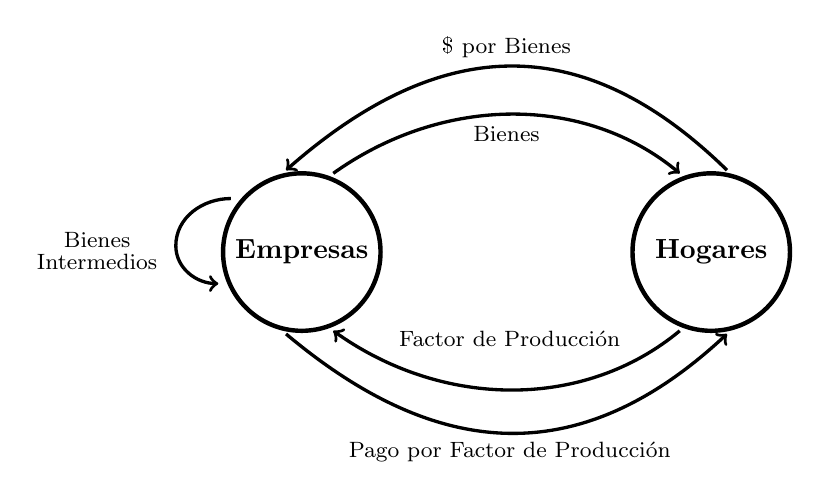
\begin{tikzpicture}[scale=0.4]
\draw[ultra thick](2,0) circle [radius =2.5];
\node[] at (2,0) { \textbf{Empresas}};
\draw[ultra thick](15,0) circle [radius =2.5];
\node[] at (15,0) {\textbf{Hogares} };
\draw [very thick, ->] (-0.25, 1.7) to [out=-180, in=90] (-2, 0.2) to [out=-90, in=180] (-0.65, -1);
\node[] at (-4.5,0.4) {\footnotesize  Bienes};
\node[] at (-4.5,-0.3) {\footnotesize  Intermedios};
\draw[very thick, ->] (3,2.5).. controls (6.5,5) and (11,5) .. (14,2.5);
\draw[very thick, <-] (1.5,2.6).. controls (6.5,7) and (11,7) .. (15.5,2.6);
\node[] at (8.5,3.75) {\footnotesize  Bienes};
\node[] at (8.5,6.5) {\footnotesize  \$ por Bienes};
\draw[very thick, <-] (3,-2.5).. controls (6.5,-5) and (11,-5) .. (14,-2.5);
\draw[very thick, ->] (1.5,-2.6).. controls (6.5,-6.8) and (11,-6.8) .. (15.5,-2.6);
\node[] at (8.6,-2.75) {\footnotesize  Factor de Producción};
\node[] at (8.6,-6.35) {\footnotesize Pago por Factor de Producción};
\end{tikzpicture}
\label{fig:25.1}
\end{figure} 

\end{frame}


\begin{frame}{Definiendo el PBI}
\begin{itemize}
   \item El PBI es el valor de mercado de los bienes finales producidos en un peridodo de tiempo en un pais
   \item Notese que la suma de los bienes es igual a la suma de los ingresos!
   \item Por eso aveces nos referimos al PBI como ingreso nacional.
   \end{itemize}
\end{frame}


\begin{frame}{Midiendo el PBI}
    \begin{itemize}
        \item Tenemos tres maneras de medirlo
       \begin{itemize}
           \item Por el gasto (valor de los bienes finales consumidos)
           \item Por los ingresos (suma de los ingresos recibidos)
           \item Por la suma de los valores agregados 
       \end{itemize}
    \end{itemize}
\end{frame}

\begin{frame}{Medición del PBI}
    \begin{figure} [H]   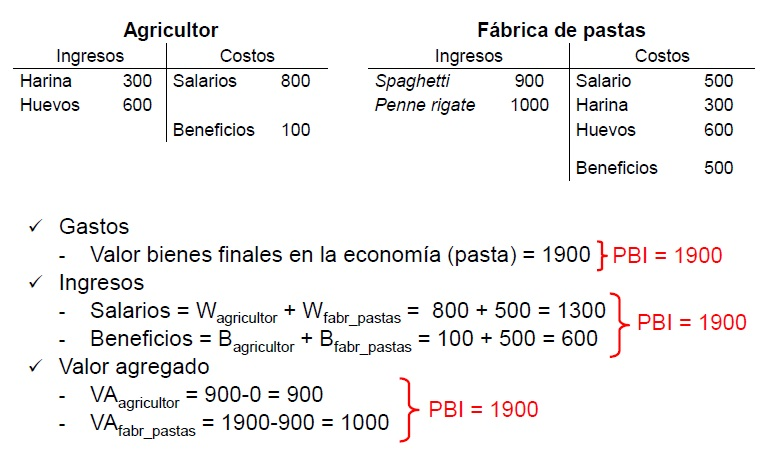
\includegraphics[scale=0.55]{images/C16.2.jpg}
\label{fig:25.2}
\end{figure}

\end{frame}



\begin{frame}{Buscando los datos}
    \begin{itemize}
        \item Cada país tiene su agencia de estadísticas
        \item En Argentina es el Indec
        \item Pueden ver también Alphacast
        \item Para bases de datos homogéneas IFS
        \item Para perspectivas futuras WEO
        \item Para otra visión Fred
        
    \end{itemize}
\end{frame}


\begin{frame}{Temas en la medición del PBI}
    \begin{itemize}
        \item Bienes ya producidos no van
        \item Transferencias de ingresos no van
        \item Planes sociales?
        \item Economia informal si
        \item Gasto publico al costo
        \item Productos de internet y ajustes por calidad
    \end{itemize}
\end{frame}

\begin{frame}{PBI y PBN}
    \begin{itemize}
        \item El Producto Bruto Nacional (PBN) es el PBI ajustado por el retorno a los factores externos
    \end{itemize}
    \begin{table}[H]
\begin{tabular}{|c|c|c|c|}
\hline
\multicolumn{2}{|c|}{\textbf{Top PBI}} & \multicolumn{2}{c|}{\textbf{Top PNB}} \\ \hline
1. Luxembourg              & 116.921   & 1.  Macao                  & 116.080  \\ \hline
2.  Switzerland            & 86.849    & 2. Qatar                   & 91.499   \\ \hline
\textbf{3. Ireland}        & 83.849    & 3.  Singapore              & 87.735   \\ \hline
4. Norway                  & 67.176    & 4. Bermuda                 & 85.191   \\ \hline
5. United States           & 63.415    & 5. Luxembourg              & 72.145   \\ \hline
6. Brunei Darussalam       & 59.123    & 6. Switzerland             & 68.992   \\ \hline
7. Hong kong               & 56.420    & 7.  United Arab Emirates   & 67.462   \\ \hline
8. Denmark                 & 55.864    & 8. Norway                  & 66.749   \\ \hline
9. United Arab Emirates    & 55.693    & \textbf{9. Ireland}        & 66.668   \\ \hline
10. San Marino             & 55.384    & 10. Brunei Darussalam      & 63.963   \\ \hline
\end{tabular}
\caption{Posición de Irlanda por PBI y por PNB per capita}
\label{Tab:T38.1}
\end{table}
\end{frame}



\begin{frame}{Un caso extraordinario }
    
\begin{figure} [H]
\centering
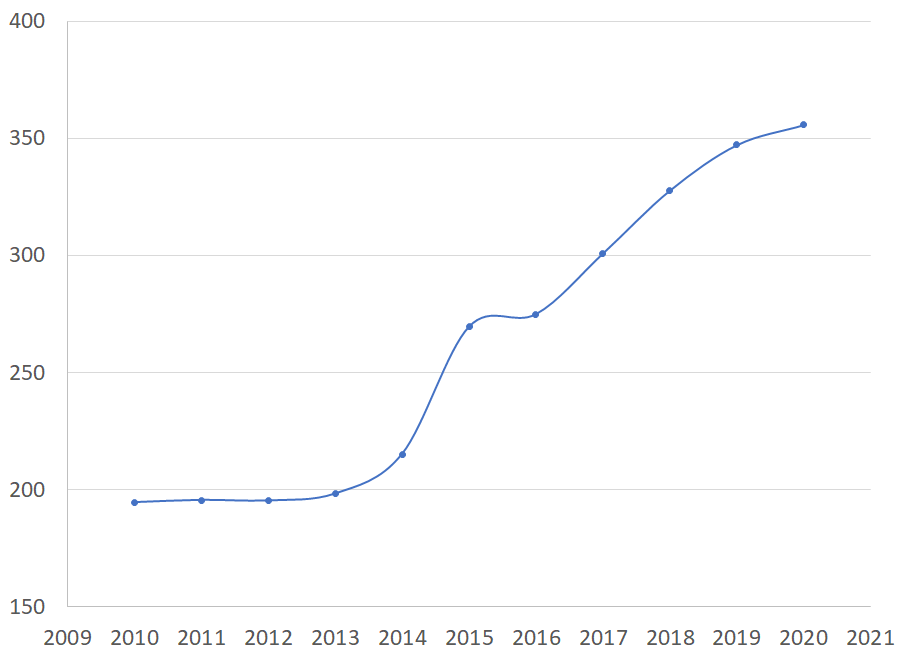
\includegraphics[]{images/G1.png}
\caption{PBI Irlanda a precios constantes}
\label{fig:G1}
\end{figure} 
\end{frame}

\begin{frame}{Graficando el PBI}
    \begin{figure} [H]   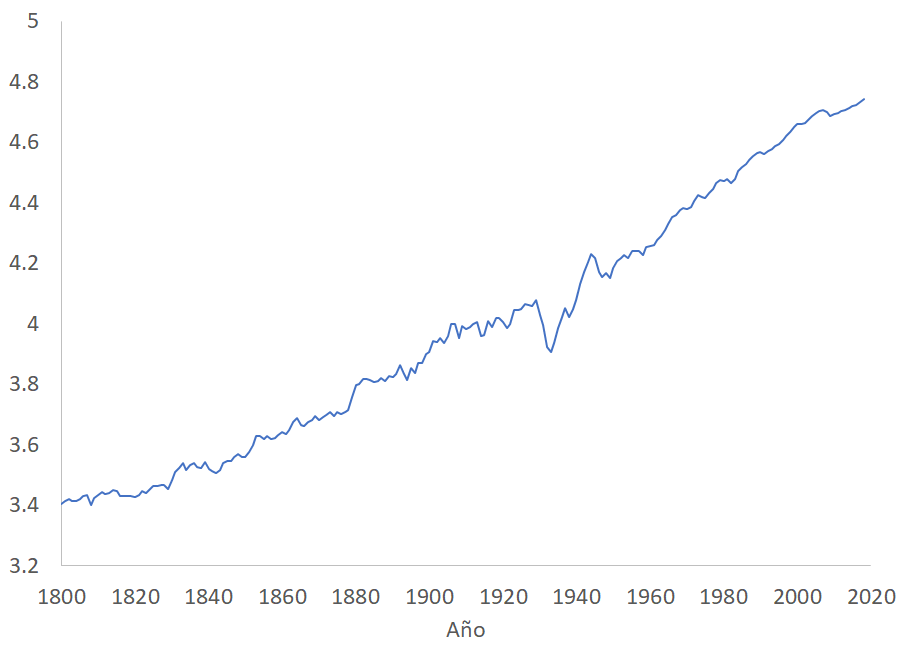
\includegraphics[scale=1]{images/G2.png}
\caption{PBI EEUU Largo Plazo}
\label{fig:25.3}
\end{figure}
\end{frame}

\begin{frame}{Ajustando con logs}
    \begin{center}
\begin{figure}[H]
\renewcommand{\figurename}{Figure}
\begin{center}
    \begin{minipage}[b]{0.35\textwidth}
        \begin{center}
\begin{tikzpicture}[scale=0.4]
\draw[very thick,<->] (0,11) node[left]{$f$}--(0,0)--(11,0) node[below]{$x$};
\draw[semithick] (0,1).. controls (3,1) and (8, 1.1) .. (8.5, 8) node [right]{\footnotesize $Ae^{\lambda x}$};
\end{tikzpicture}
\end{center}
     \end{minipage}
  %  \hfill
    \begin{minipage}[b]{0.4\textwidth}
    \begin{center}
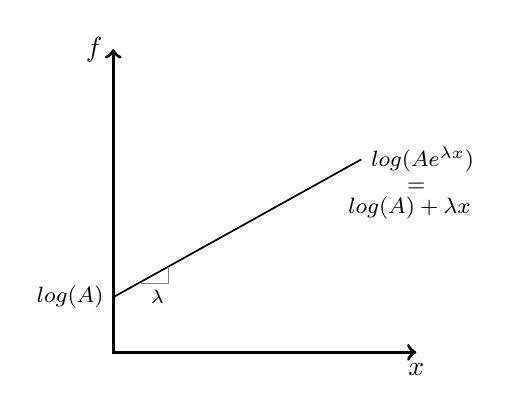
\begin{tikzpicture}[scale=0.35]
\draw[very thick,<->] (0,11) node[left]{$f$}--(0,0)--(11,0) node[below]{$x$};
\draw[semithick] (0,2)--(9, 7) node [right]{\footnotesize $log(Ae^{\lambda x})$};
\draw[semithick, gray] (1,2.5)--(2,2.5)--(2,3.1);
\node[] at (1.6,2) {\scriptsize $\lambda$};
\node[left] at (0,2) {\footnotesize $log(A)$};
\node[] at (11,6) {\footnotesize $=$};
\node[] at (10.75,5.25) {\footnotesize $log(A)+\lambda x$};
\end{tikzpicture}
\end{center}
    \end{minipage}
\end{center}
\caption{\textbf{Visiones sobre la curva de oferta}}
\label{fig:25.exp.log}
\end{figure}
\end{center} 
\end{frame}



\begin{frame}{Re-graficando}
   \begin{figure} [H]   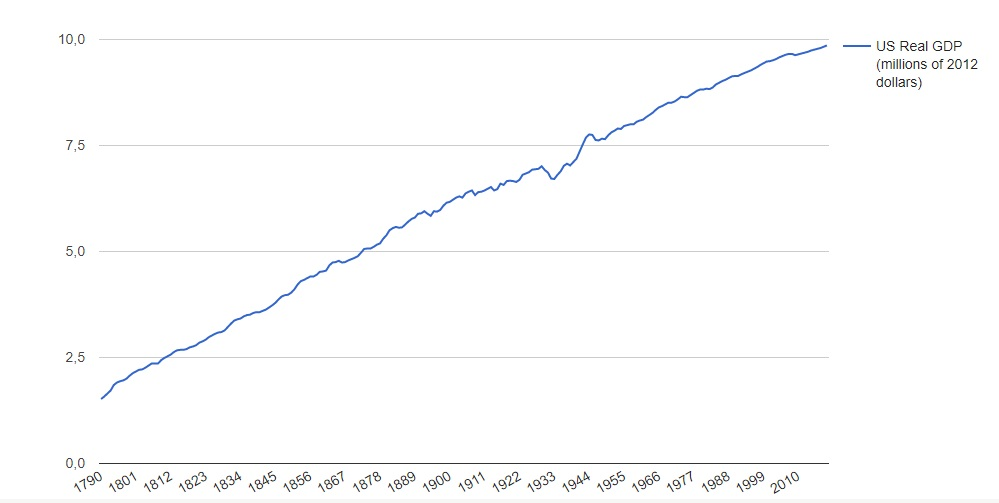
\includegraphics[scale=0.45]{images/C16.4.jpg}
\caption{PBI EEUU Largo Plazo en logaritmo}
\label{fig:16.4}
\end{figure}
%Actualizar formato 
\end{frame}



\begin{frame}{PBI nominal y real}
   
$$PBI_{NOMINAL}^{i} = p_1^{i}q_1^{i} + p_2^{i}q_2^{i} + … + p_N^{i}q_N^{i}$$
$$PBI_{NOMINAL}^{j} = p_1^{j}q_1^{j} + p_2^{j}q_2^{j} + … + p_N^{j}q_N^{j}$$,
el PBI real dejará los precios constantes de un año base cualquiera ($b$).

$$PBI_{REAL}^{i} = p_1^{b}q_1^{i} + p_2^{b}q_2^{i} + … + p_N^{b}q_N^{i}$$
$$PBI_{REAL}^{j} = p_1^{b}q_1^{j} + p_2^{b}q_2^{j} + … + p_N^{b}q_N^{j}$$.
\end{frame}


\begin{frame}{PBI nominal y real de EEUU}
    \begin{figure} [H]   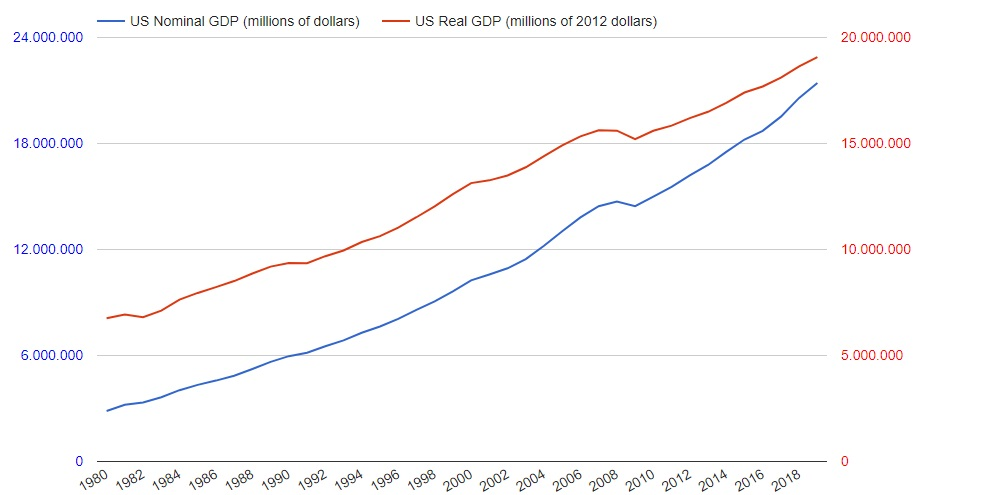
\includegraphics[scale=0.5]{images/C16.5.jpg}
\label{fig:25.5}
\end{figure}
\end{frame}
 

\begin{frame}{PBI Nominal y real de Argentina}
    \begin{figure} [H]   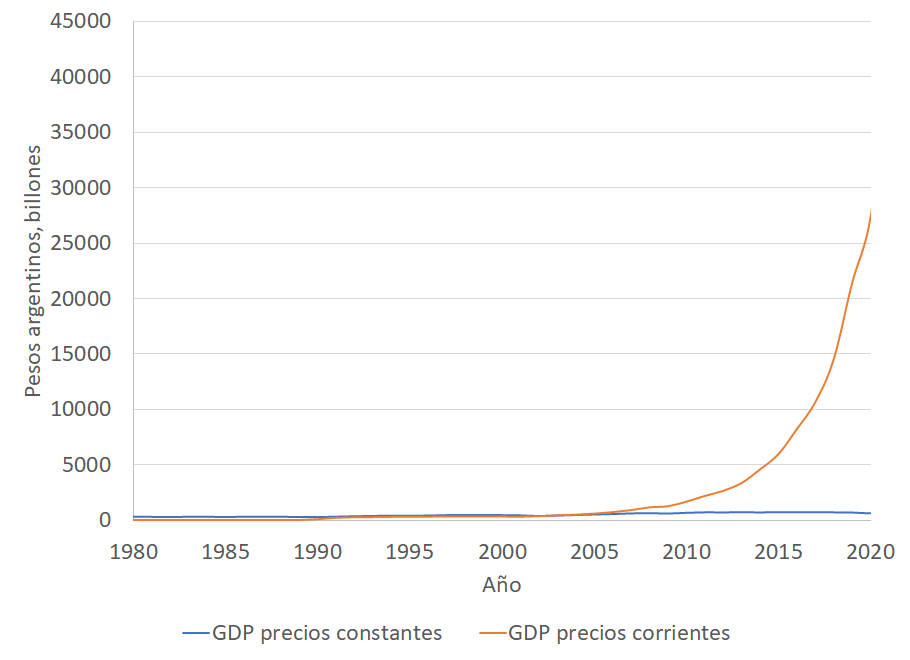
\includegraphics[scale=1.1]{images/G2B.png}

\label{fig:G2}
\end{figure}
\end{frame}


\begin{frame}{Componentes y desglose del PBI}
    \begin{itemize}
    \item Haciendo referencia a los sectores que los producen. Esto es si se originan en la agricultura, la minería, la industria, el comercio, el turismo, etc. A esta referencia la llamaremos el \textit{PBI por el lado de la oferta}. 
    \item Según el uso de estos bienes. En este caso vamos a segmentar el PBI según los bienes se usan para el consumo, la  inversión, el consumo público, el sector externo o la acumulación de inventarios. A esto lo llamaremos el \textit{PBI por el lado de la demanda}. 
\end{itemize}
\end{frame}

\begin{frame}{El PBI por el lado de la oferta}
    \begin{table}[H] 
\resizebox{.62\textwidth}{!}{%
\begin{tabular}{|c|c|}
\hline
\textbf{Elementos del PBI - Oferta}                                                                               & \textbf{Millones de pesos corrientes} \\ \hline
\begin{tabular}[c]{@{}c@{}}A - Agricultura, ganadería, caza \\ y silvicultura\end{tabular}                        & 1.543.784                             \\ \hline
B - Pesca                                                                                                         & 86.525                                \\ \hline
\begin{tabular}[c]{@{}c@{}}C - Explotación de minas \\ y canteras\end{tabular}                                    & 857.865                               \\ \hline
D - Industria manufacturera                                                                                       & 4.223.679                             \\ \hline
E - Electricidad, gas y agua                                                                                      & 438.732                               \\ \hline
F - Construcción                                                                                                  & 885.981                               \\ \hline
\begin{tabular}[c]{@{}c@{}}G - Comercio mayorista, minorista \\ y reparaciones\end{tabular}                       & 4.451.862                             \\ \hline
H - Hoteles y restaurantes                                                                                        & 312.971                               \\ \hline
\begin{tabular}[c]{@{}c@{}}I - Transporte, almacenamiento \\ y comunicaciones\end{tabular}                        & 1.320.842                             \\ \hline
J - Intermediación financiera                                                                                     & 999.990                               \\ \hline
\begin{tabular}[c]{@{}c@{}}K - Actividades inmobiliarias, \\ empresariales y de alquiler\end{tabular}             & 2.655.948                             \\ \hline
L - Administración pública y defensa                                                                              & 1.890.537                             \\ \hline
M - Enseñanza                                                                                                     & 1.457.592                             \\ \hline
N - Servicios sociales y de salud                                                                                 & 1.237.435                             \\ \hline
\begin{tabular}[c]{@{}c@{}}O - Otras actividades de servicios \\ comunitarias, sociales y personales\end{tabular} & 524.134                               \\ \hline
\begin{tabular}[c]{@{}c@{}}P - Hogares privados con servicio \\ doméstico\end{tabular}                            & 157.032                               \\ \hline
\end{tabular}%
}
\caption{PBI Argentina 2020 - Oferta}
\label{Tab:T38.3}
\end{table}
\end{frame}

\begin{frame}{El PBI por el lado de la demanda}
    \begin{table}[H]
\begin{tabular}{|c|c|}
\hline
\textbf{Elementos del PBI - Demanda} & \textbf{Millones de pesos corrientes} \\ \hline
Consumo privado                      & 17.456.121                            \\ \hline
Consumo publico                      & 4.268.255                             \\ \hline
Exportaciones                        & 4.559.670                             \\ \hline
Importaciones                        & 3.725.473                             \\ \hline
Formación bruta de capital fijo      & 3.816.717                             \\ \hline
\end{tabular}
\caption{PBI Argentina 2020 - Demanda}
\label{Tab:T38.2}
\end{table}

\end{frame}



\begin{frame}{El PBI por la demanda}
    
  \begin{equation}
        Y= C + I + G + X - M +  \Delta Inv.
  \end{equation}
  \begin{itemize}
  \item Esta es una ecuación muy conocida en macroeconomía
  \end{itemize}
\end{frame}

\begin{frame}{¿Cómo se compara el PBI entre países?}
    \begin{figure} [H]   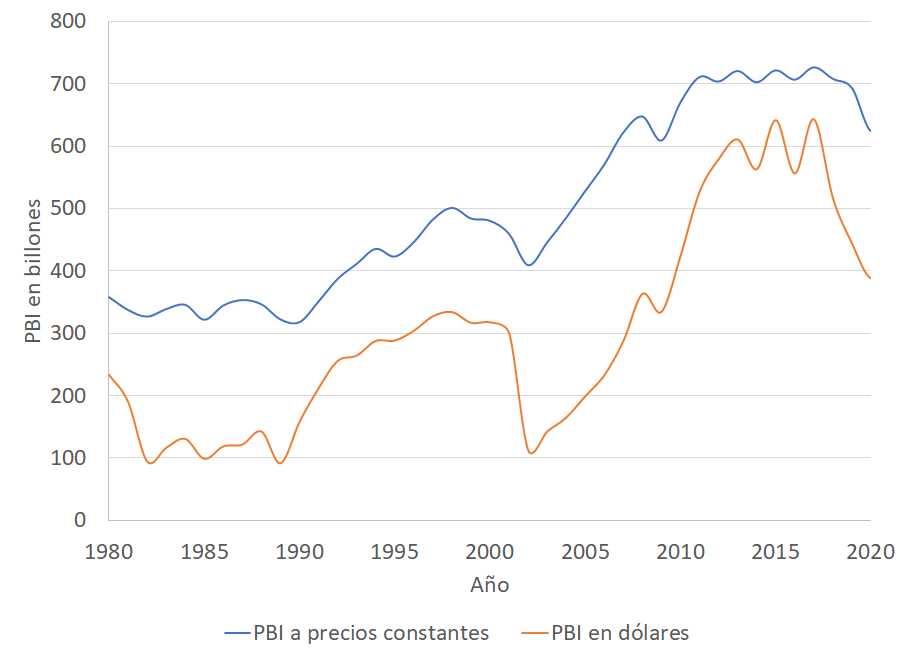
\includegraphics[scale=1.04]{images/G3.png}
\caption{PBI real y PBI en dolares de Argentina}
\label{fig:G66}
\end{figure}
\end{frame}
                   
\begin{frame}{PBI en dolares y PBI en PPP}
\begin{itemize}
    \item PBI de EEUU es 59041
    \item PBI de India es 142.073 rupias
    \item PBI de India en dolares 965 dolares
    \item Una mejor medida es el PBI de India medido en los precios de EEUU
    \item Con ese calculo el PBI PPP de India es de 6461!
\end{itemize}
    
\end{frame}


\begin{frame}{Una corporación India-China-EEUU}
   \begin{figure}[H]
\centering
    \subfigure{
\resizebox{0.42\textwidth}{!}{%
    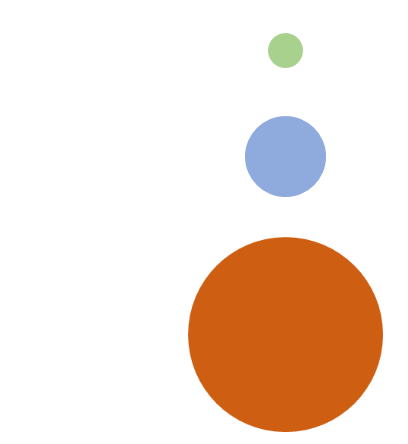
\includegraphics[width=0.9\textwidth]{images/G4.2A.png}}}
  \hfill 
    \subfigure{
\resizebox{0.42\textwidth}{!}{%
    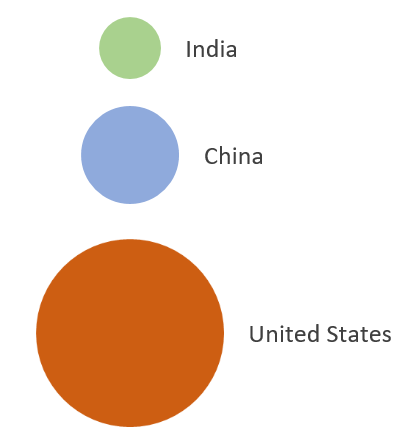
\includegraphics[width=0.9\textwidth]{images/G4.2B.png}}}
\caption{\textbf{PBI en dolares vs PPP}}
\end{figure} 
\end{frame}

\begin{frame}{Otra comparación}
    \begin{figure} [H]   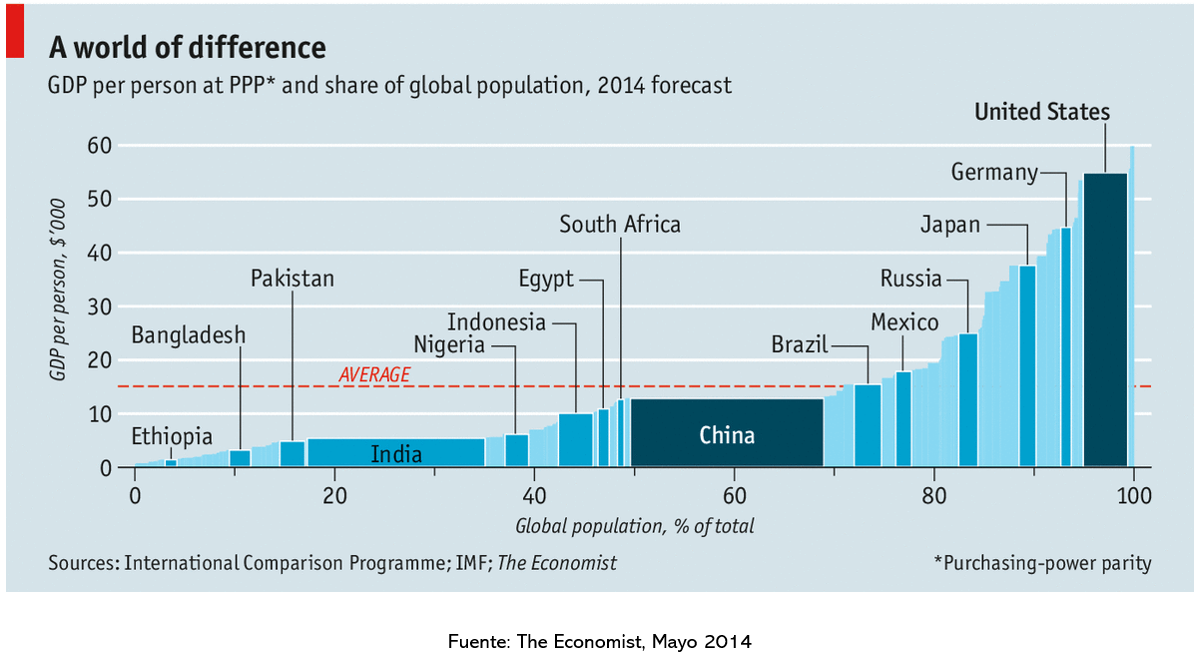
\includegraphics[scale=0.5]{images/C16.6.png}
\caption{\textbf{¿Cómo comparamos los ingresos en el mundo?}}
\label{fig:16.6}
\end{figure}

\end{frame}


\begin{frame}{Índice de desarrollo humano}
    De hecho, las Naciones Unidas (ONU) hicieron justamente esto al crear el Índice de Desarrollo Humano que está conformado por tres indicadores claves: 

\begin{itemize}
    \item Ingresos (PBI per cápita ajustado por PPP)
\item Longevidad (esperanza de vida al nacer)
\item Conocimiento (alfabetización y años de estudio).
\end{itemize}
\end{frame}


\begin{frame}{Indice de desarrollo humano}
    
\begin{figure} [H]  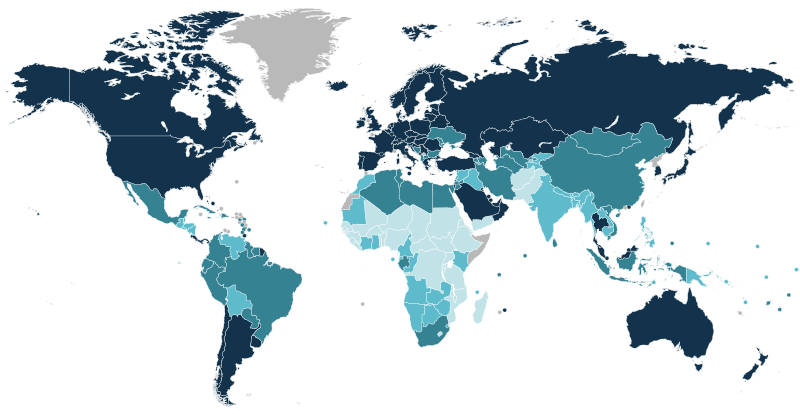
\includegraphics[scale=0.5]{images/C16.7.png}
\caption{\textbf{Índice de Desarrollo Humano HDI 2019}}
\label{fig:25.7}
\end{figure}
\end{frame}


\begin{frame}{Midiendo la inflacion}
\begin{itemize}    
\item Típicamente para medirlo se elige una canasta de bienes. Definida la canasta de bienes, el nivel de precios es: 

\begin{equation}
P_t = p_1 q_1^c+ p_2 q_2^c...p_n q_n^c,
\end{equation}

\item donde $q_i^c$ es la participación del bien $i$ en la canasta de consumo que se considera. A su vez la tasa de inflación sería 

\begin{equation}
\pi =\frac{P_t - P_{t-1}}{P_{t-1}}= \frac{\vartriangle P}{P_{t-1}}.
\end{equation}
\end{itemize}
\end{frame}

\begin{frame}{Problemas con el indice}
    \begin{itemize}
        \item Eligiendo la canasta
        \item Ajustando por calidad
        \item Sesgo de sustitución
        \item Sesgo de subreporte
        \item Hay distintos tipos de índices de precios (consumidor, construcción, etc.)
    \end{itemize}
\end{frame}




\begin{frame}{Deflactor del PBI }
\begin{itemize}
\item Existe una medida de precios del conjunto de bienes de la economía? 
\item Si, lo llamamos el deflactor del PBI
\item 
  \begin{equation}
    PBI_{DEFLACTOR}^{i}=\frac{PBI_{NOMINAL}^{i}}{PBI_{REAL}^{i}}\quad x 100.
\end{equation} 
\end{itemize}
\end{frame}

\begin{frame}{Teoria del crecimiento}
    \begin{figure} [H]   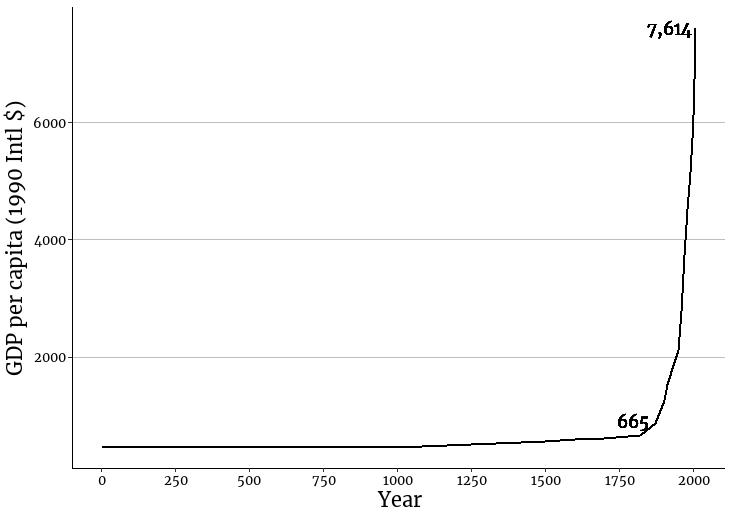
\includegraphics[scale=0.55]{images/C17.1.png}
\caption{\textbf{Crecimiento de la Humanidad}}
\label{fig:26.1}
\end{figure}
\end{frame}


\begin{frame}{Que genero el crecimiento explosivo?}
    \begin{itemize}
    \item \textbf{Revolución industrial}: la máquina a vapor generó una potencialidad de expansión en la producción junto con los ferrocarriles y la industria textil produjeron un aumento en el nivel de vida sin precedentes. 
    \item \textbf{Revolución francesa}: permitió la movilidad social y otorgó a las personas mayor libertad para elegir los trabajos y ocupaciones según sus preferencias y capacidades. Se pasó de una sociedad estamentaria a una sociedad libre. Fue una revolución en el uso del factor humano liberando a la gente de sus ataduras medievales. 
    \item \textbf{Constitución de EEUU}: Quedaba claro el contraste con el poder absolutista de los monarcas europeos. Contenía fuertes restricciones al Estado y lo que éste podía hacer. La emergencia de los gobiernos republicanos con división de poderes implicó un cambio radical en la calidad de la gestión de los recursos públicos.  
\end{itemize}
\end{frame}

\begin{frame}{Felicidad y nivel de ingreso}
    \begin{figure} [H]   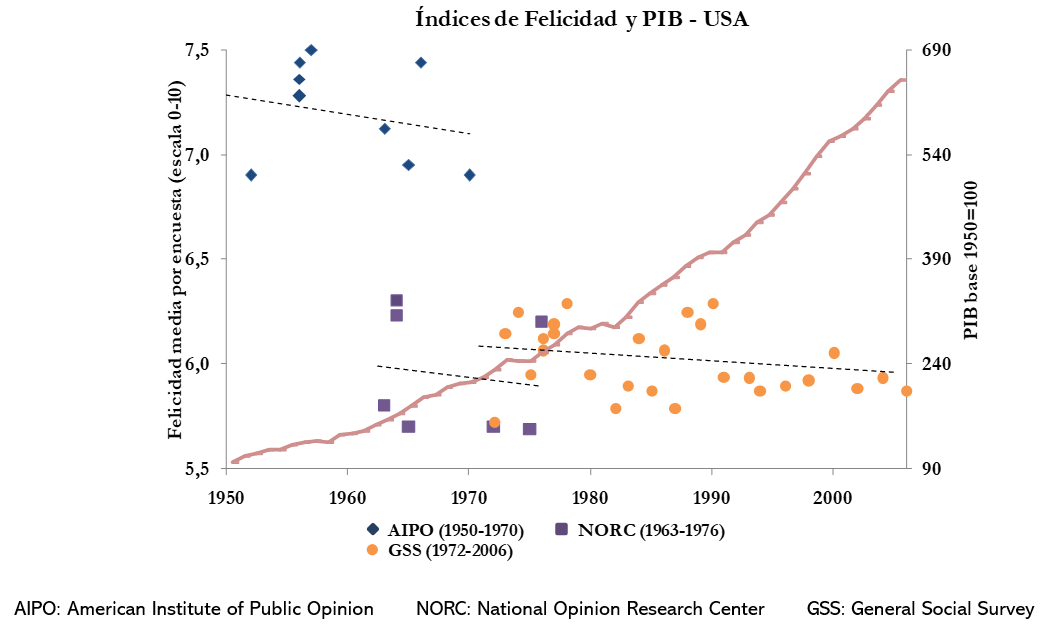
\includegraphics[scale=0.55]{images/C17.2.png}
\caption{\textbf{Felicidad y nivel de ingreso}}
\label{fig:26.2}
\end{figure}
\end{frame}


\begin{frame}{La aceleracion del crecimiento en graficos}
    \begin{figure}[htp]
\href{https://www.gapminder.org/tools/} {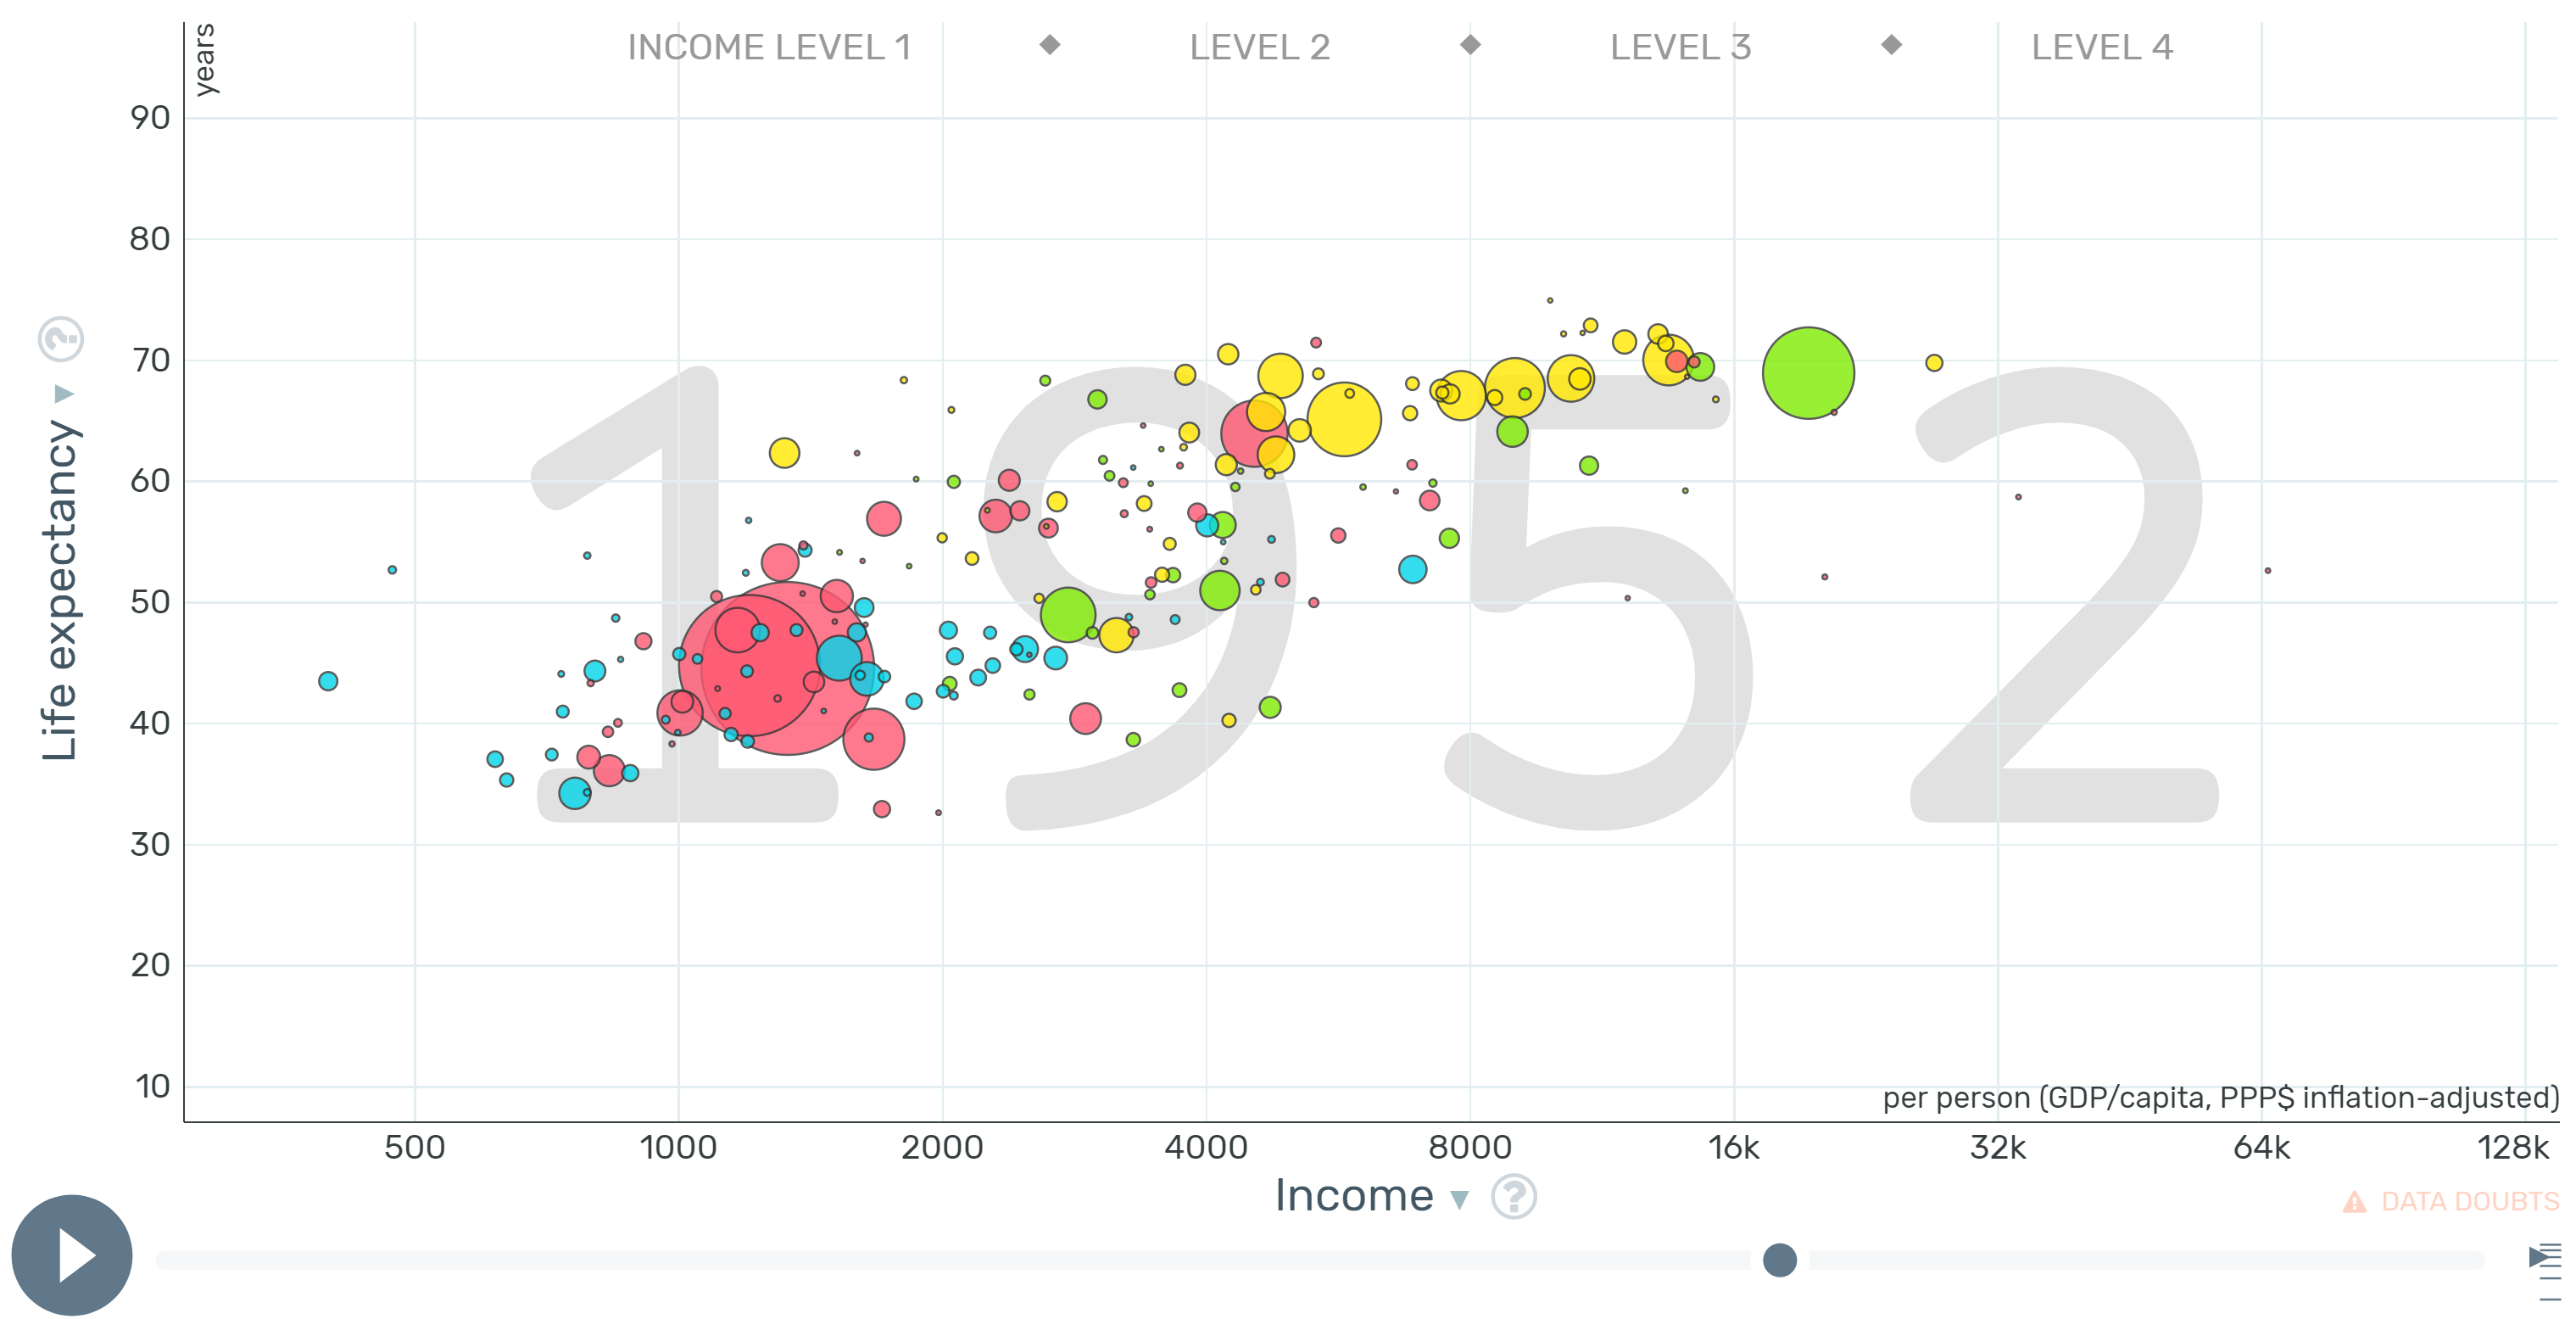
\includegraphics[width=0.99\textwidth]{images/Gapminder.png}} 
\end{figure}
\end{frame}




\begin{frame}{Fuentes del crecimiento}
   \begin{equation}
    Y = AF(K,L,H,RN),
\end{equation} 
\begin{itemize}
    \item El crecimiento viene de la acumulacion de factores o de la tecnologia?
    \item El hallazgo de Solow
    \item Hong Kong vs Singapur
\end{itemize}
\end{frame}

\begin{frame}{Un ejemplo de productividad}
    \begin{figure} [H]   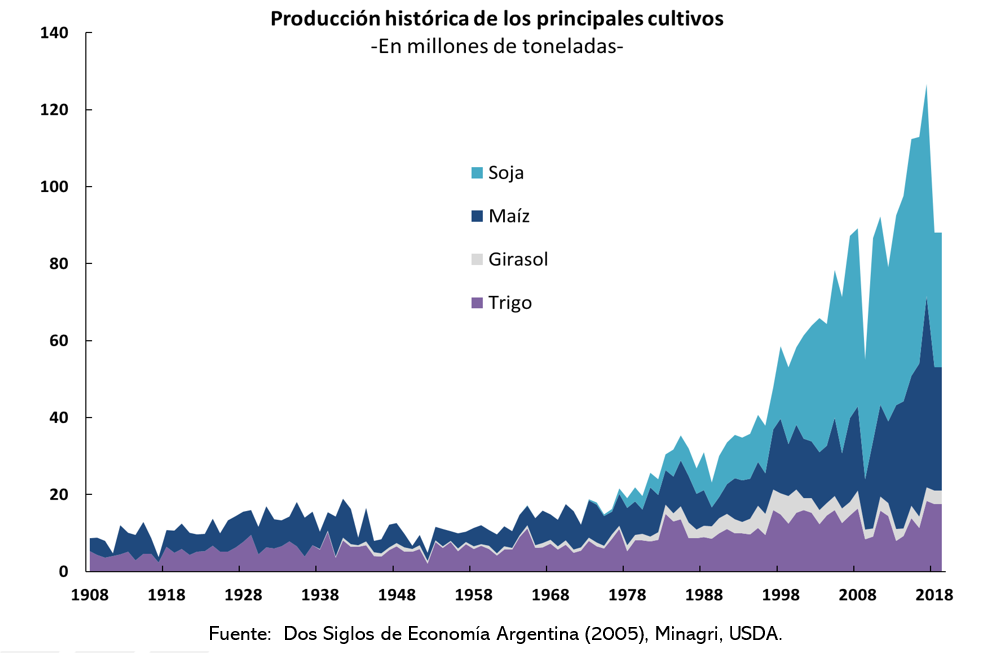
\includegraphics[scale=0.55]{images/C17.3.png}
\label{fig:17.3}
\end{figure}
\end{frame}


\begin{frame}{La descomposicion de crecimiento para Argentina}
    \begin{figure} [H]   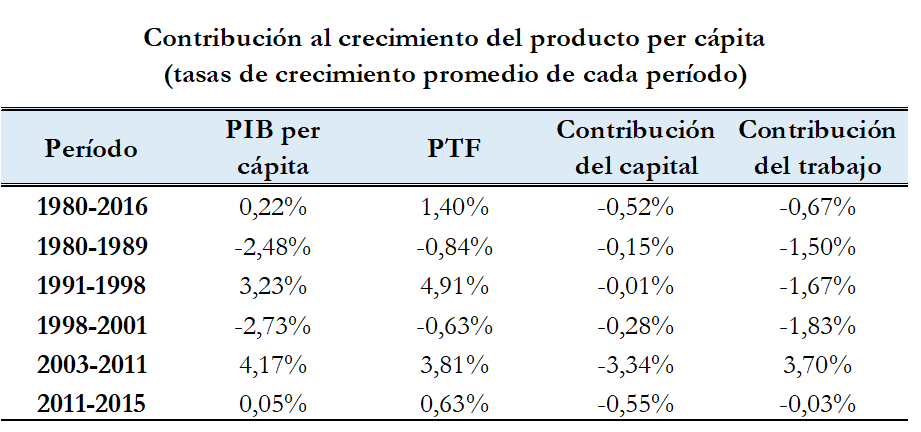
\includegraphics[scale=0.55]{images/C17.4.png}
\caption{\textbf{Descomposición del crecimiento de Argentina}}
\label{fig:26.4}
\end{figure}
\end{frame}



\begin{frame}{Instituciones}
    
\begin{figure}[H]
\begin{center}
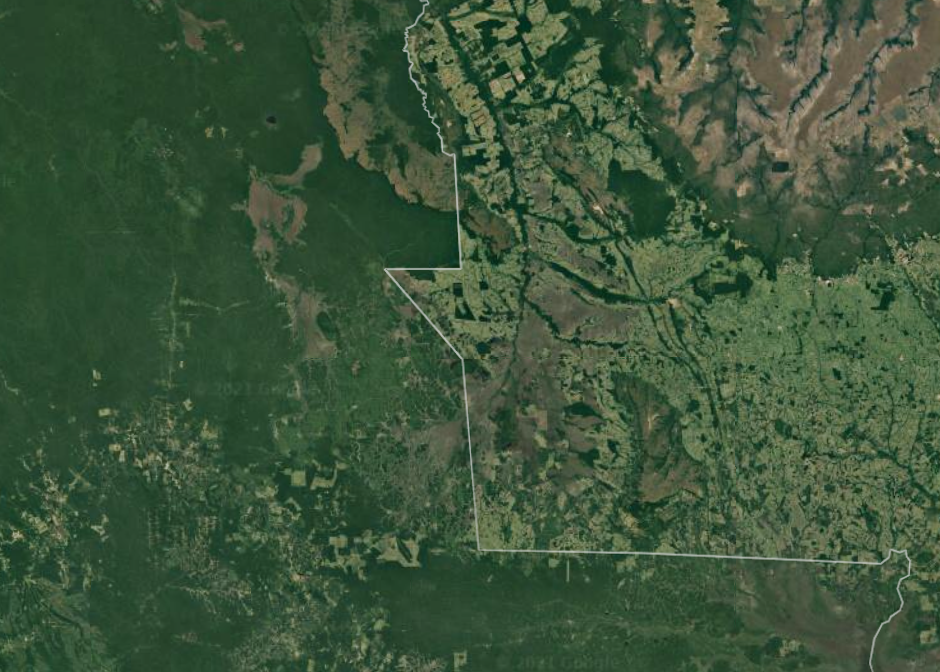
\includegraphics[width=0.8\textwidth]{images/C26.2.png}
\end{center}
\caption{\textbf{Frontera entre Bolivia (izquierda) y Brazil}}
\label{fig:border_bol_bra}
\end{figure}
\end{frame}

\begin{frame}{Instituciones}
    \begin{figure}[H]
\begin{center}
\includegraphics[width=0.8\textwidth]{images/C26.3.png}
\end{center}
\caption{\textbf{Península de Corea de noche}}
\label{fig:korea}
\end{figure}

\end{frame}

\begin{frame}{La distribución del ingreso la curva de Lorenz}
    \begin{figure} [H]
\centering
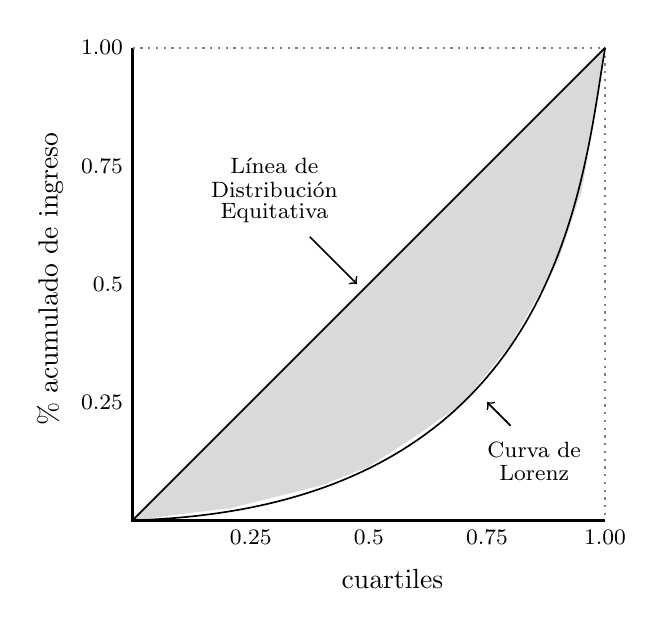
\begin{tikzpicture}[scale=0.6]
\draw[fill,gray!30] (0,0)--(10,10)--(9.5,7)--(9,5.5)--(8,3.75)--(7,2.5)--(6,1.8)--(5,1.15)--(4,0.75)--(2,0.25);
\draw[very thick,-] (0,10) node[above]{}--(0,0)--(10,0) node[right]{};
\draw[thick, dotted, gray] (0,10)--(10,10)--(10,0);
\draw[semithick] (0,0)--(10,10);
\draw[semithick] (0,0)..controls (9,0.25) and (9.5,7)..(10,10);
\node at (-1.75, 5){\rotatebox{90}{ \% acumulado de ingreso}};
\node[] at (5.5,-1.25) { cuartiles};
\node[below] at (2.5,0){\footnotesize 0.25};
\node[below] at (5,0){\footnotesize 0.5};
\node[below] at (7.5,0){\footnotesize 0.75};
\node[below] at (10,0){\footnotesize 1.00};
\node[left] at (0,2.5){\footnotesize 0.25};
\node[left] at (0,5){\footnotesize 0.5};
\node[left] at (0,7.5){\footnotesize 0.75};
\node[left] at (0,10){\footnotesize 1.00};
\node[] at (3,7.5) {\footnotesize Línea de };
\node[] at (3,7) {\footnotesize Distribución};
\node[] at (3,6.5) {\footnotesize Equitativa };
\draw[semithick, ->] (3.75,6)--(4.75,5);
\node[] at (8.5,1.5) {\footnotesize Curva de };
\node[] at (8.5,1) {\footnotesize Lorenz };
\draw[semithick, ->] (8,2)--(7.5,2.5);
\end{tikzpicture}
\caption{Curva de Lorenz}
\label{fig:18.1}
\end{figure} 
\end{frame}



\begin{frame}{El coeficiente de Gini}
    \begin{figure} [H]
\centering
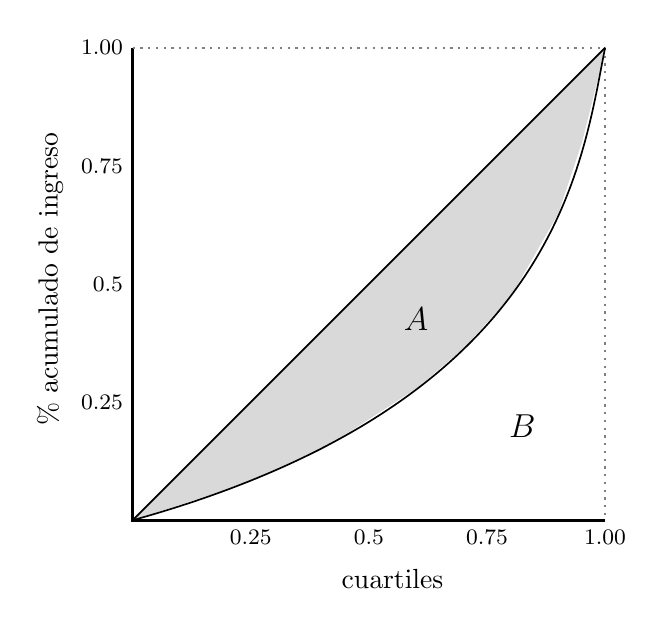
\begin{tikzpicture}[scale=0.6]
\draw[fill,gray!30] (0,0)--(10,10)--(9.5,8)--(9,6.5)--(8,4.75)--(7,3.65)--(6,2.8)--(5,2.15)--(4,1.5)--(2,0.65);
\draw[very thick,-] (0,10) node[above]{}--(0,0)--(10,0) node[right]{};
\draw[thick, dotted, gray] (0,10)--(10,10)--(10,0);
\draw[semithick] (0,0)--(10,10);
\draw[semithick] (0,0)..controls (9,2.5) and (9.5,7.5)..(10,10);
\node at (-1.75, 5){\rotatebox{90}{ \% acumulado de ingreso}};
\node[] at (5.5,-1.25) { cuartiles};
\node[below] at (2.5,0){\footnotesize 0.25};
\node[below] at (5,0){\footnotesize 0.5};
\node[below] at (7.5,0){\footnotesize 0.75};
\node[below] at (10,0){\footnotesize 1.00};
\node[left] at (0,2.5){\footnotesize 0.25};
\node[left] at (0,5){\footnotesize 0.5};
\node[left] at (0,7.5){\footnotesize 0.75};
\node[left] at (0,10){\footnotesize 1.00};
\node[] at (6,4.25) {\large $A$};
\node[] at (8.25,2) {\large $B$};
\end{tikzpicture}
\caption{Curva de Lorenz}
\label{fig:18.2}
\end{figure} 

\end{frame}

\begin{frame}{Evolución de la pobreza en el mundo}
    \begin{figure} [H]
    \centering
     \href{https://www.gapminder.org/tools/#$model$markers$bubble$encoding$frame$speed:139;;;;;&chart-type=bubbles&url=v1}{
    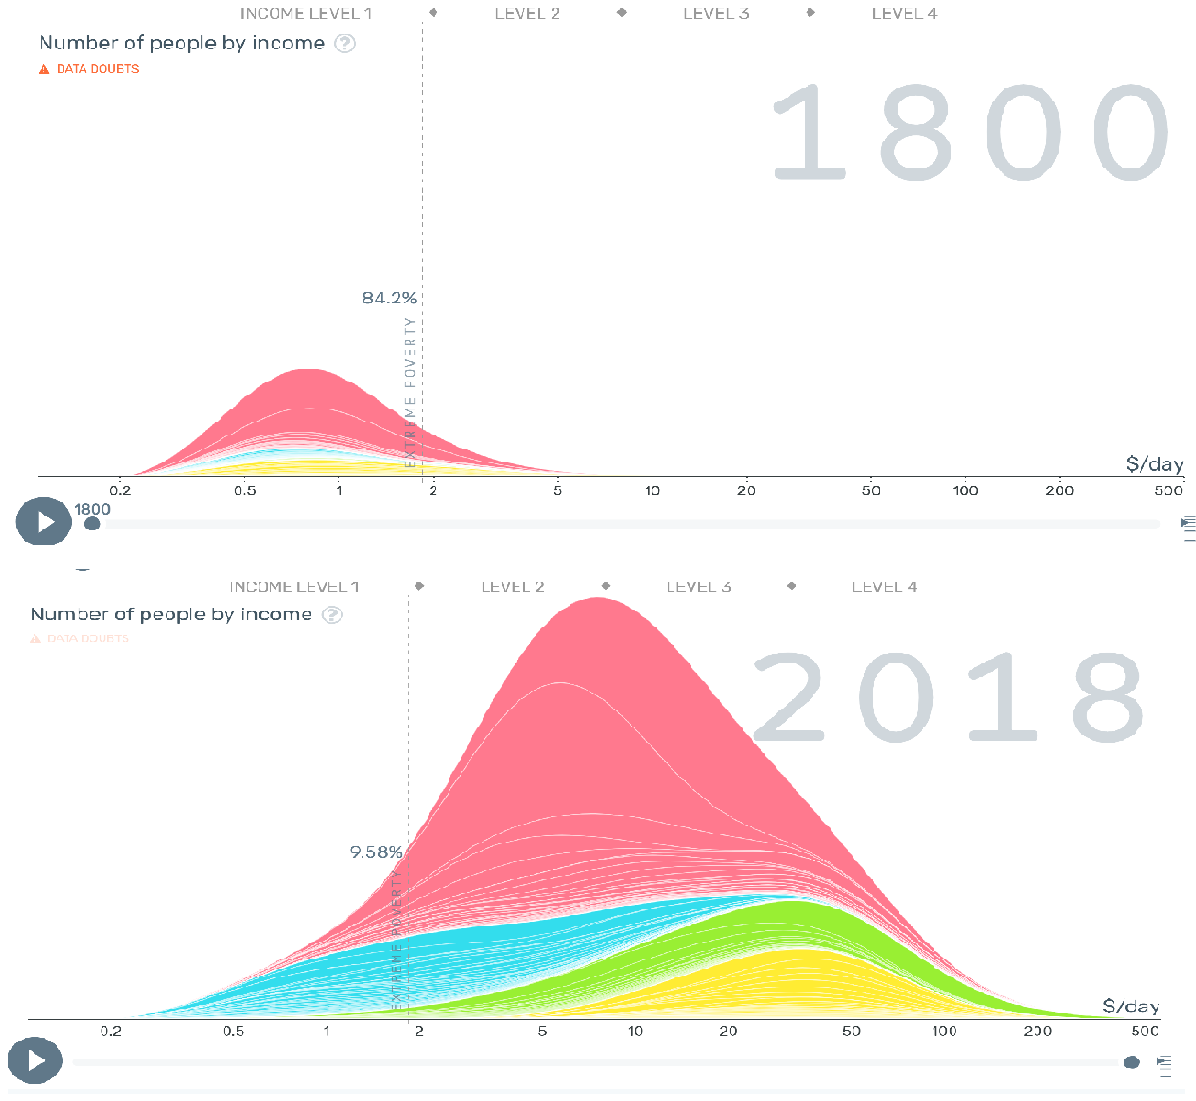
\includegraphics[scale=0.75]{images/Gapminder3.png}}
\end{figure}
\end{frame}


\begin{frame}{Discusión}
\begin{itemize}
    \item The college premium
    \item Distribución del ingreso global vs cada país
    \item El debate de Piketty
    \item El concepto de justicia de Rawls 
    \begin{itemize}
        \item Que nos dice sobre como debiera ser una estructura tributaria
    \end{itemize}
\end{itemize}
    
\end{frame}


\begin{frame}{El ciclo económico}
    \begin{figure} [H]   
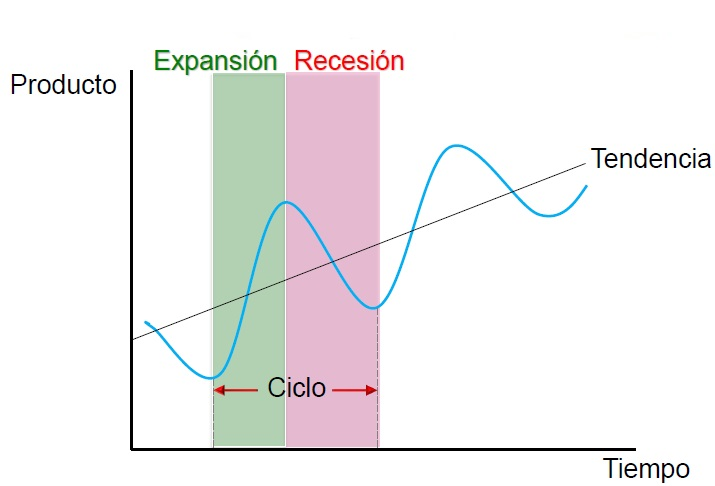
\includegraphics[scale=0.55]{images/C19.1.jpg}
\label{fig:19.1}
\end{figure}

\end{frame}


%---------------------------------------------------------------------------%

\begin{frame}{Datos con estacionalidad vs. desestacionalizados}

\centering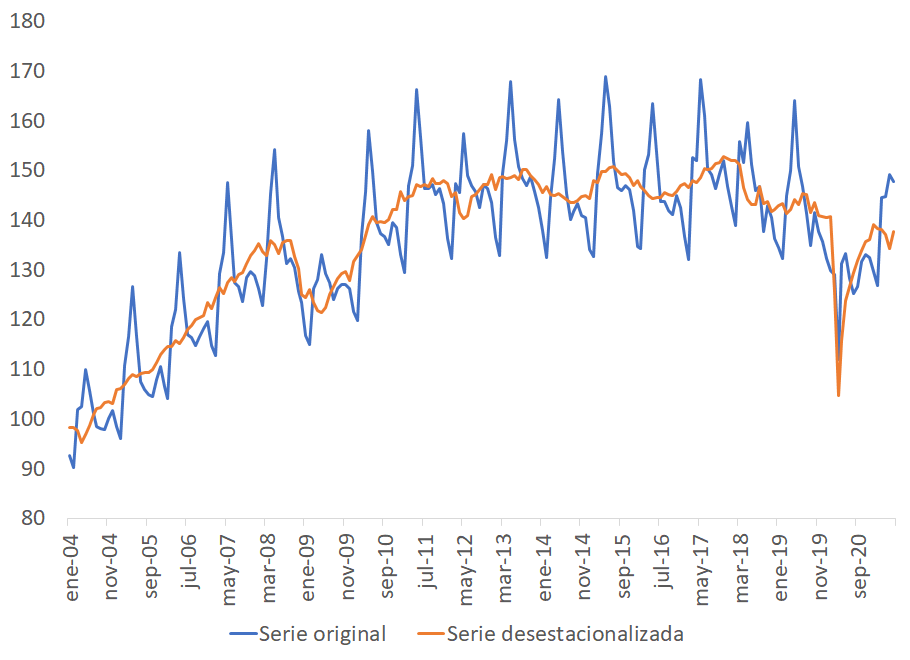
\includegraphics[width=11cm]{G11.png}\

\end{frame}

%---------------------------------------------------------------------------%

\begin{frame}{Arrastre estadístico}

\centering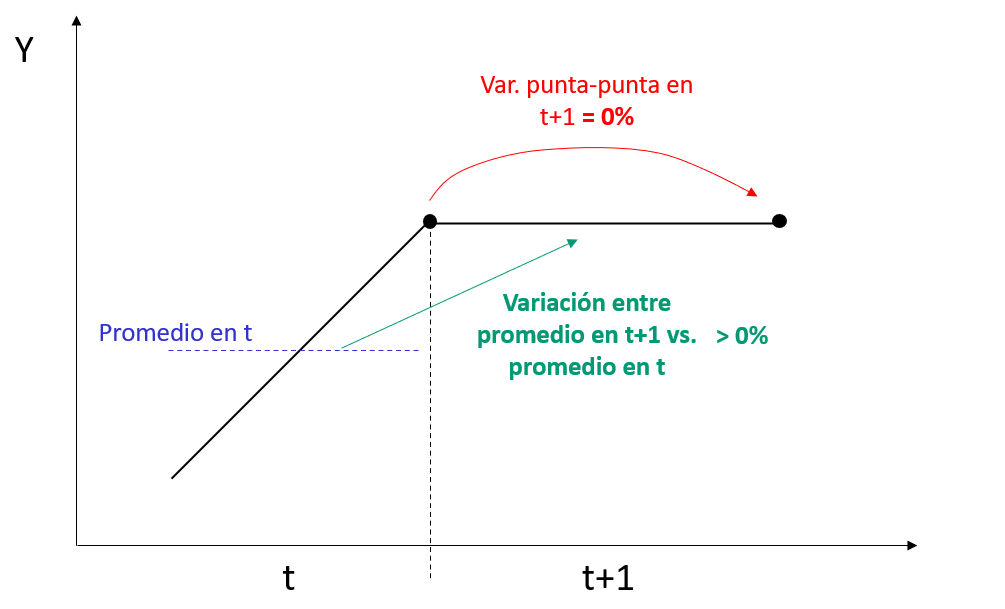
\includegraphics[width=12cm]{P11.png}\

\end{frame}


\begin{frame}{Evolución reciente del nivel de actividad}

\centering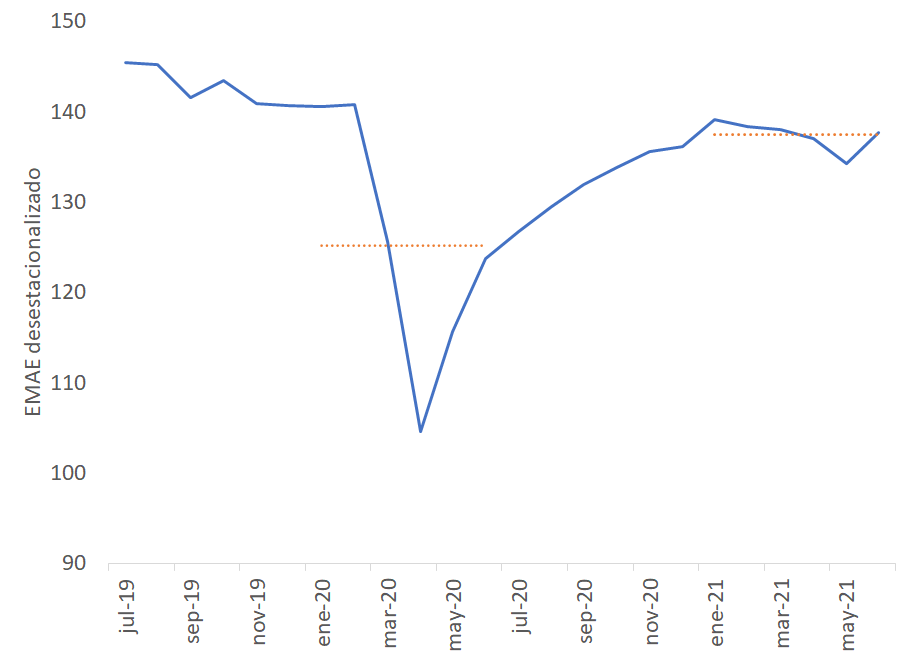
\includegraphics[width=11cm]{G12.png}\

\end{frame}

%---------------------------------------------------------------------------%


%---------------------------------------------------------------------------%


\begin{frame}{Ciclos en el PBI en EEUU}

\centering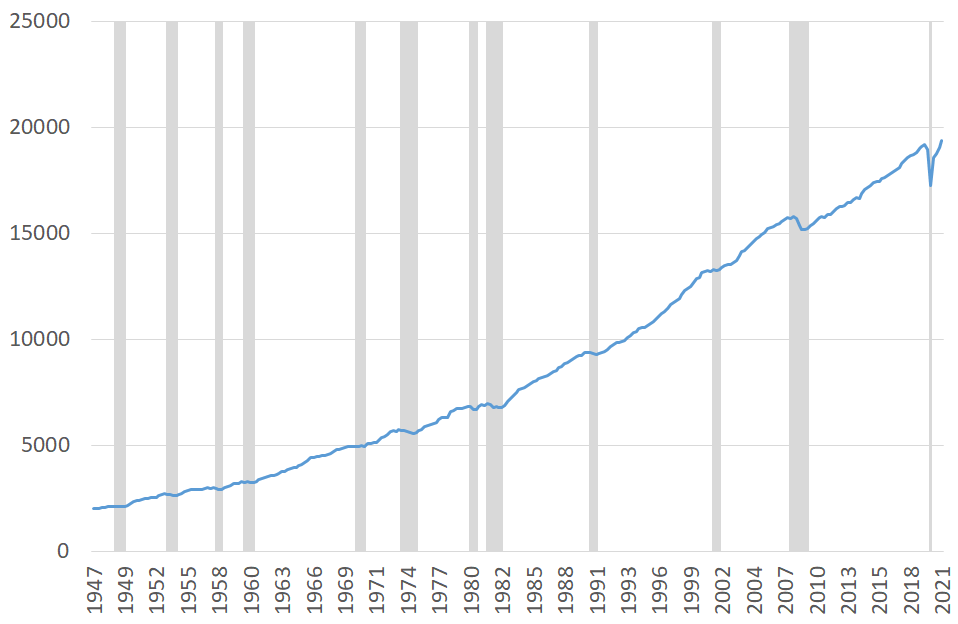
\includegraphics[width=12cm]{USA_Rec.png}\

\end{frame}

%---------------------------------------------------------------------------%

\begin{frame}{Ciclos en el PBI en Argentina}

\centering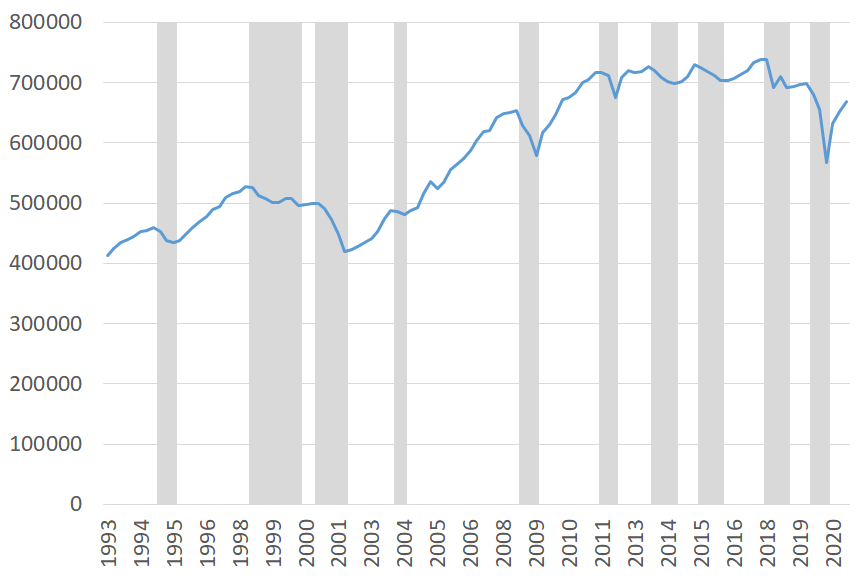
\includegraphics[width=12cm]{ARG_Rec.png}\

\end{frame}



%---------------------------------------------------------------------------%

\begin{frame}{Estimando el ciclo}

\centering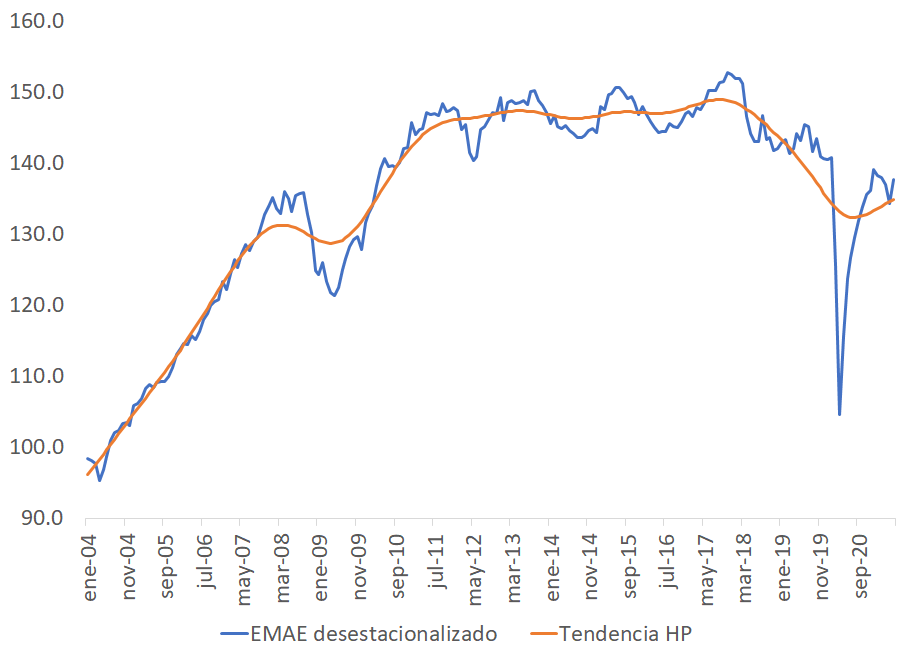
\includegraphics[width=12cm]{G9.png}\

\end{frame}

%---------------------------------------------------------------------------%

\begin{frame}{Ciclos Económicos comparados}

\centering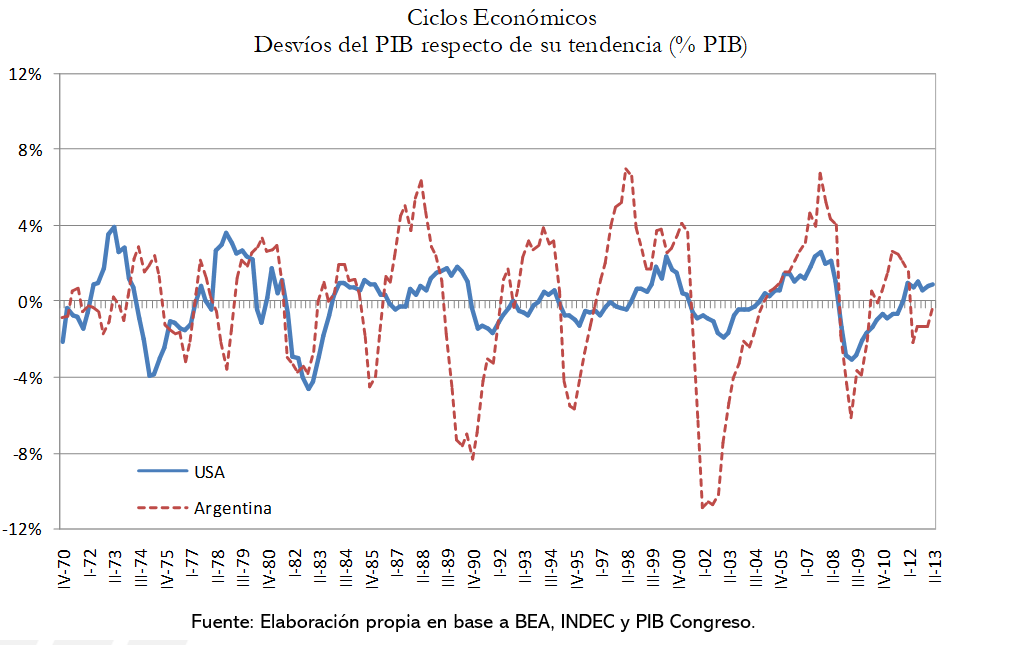
\includegraphics[width=12cm]{P12.png}\

\end{frame}




%---------------------------------------------------------------------------%

\begin{frame}{}
\centering\huge\textbf{Armando el mecano de la economía} 
\vspace{2mm}
\hrule
\end{frame}
%---------------------------------------------------------------------------%


\begin{frame}{Empezamos a armar el mecano: oferta y demanda agregada}

    \begin{itemize}
        \item Demanda Agregada \textsc{“El gasto”} \faCartPlus
        \item Oferta Agregada \textsc{"La capacidad productiva”} \faIndustry
    \end{itemize}
    \vspace{3mm}
    
    \centering
\includegraphics[width=5cm]{P17b.png}\

\end{frame}

%---------------------------------------------------------------------------%

\begin{frame}{¿Cómo se determina el producto?}

    \begin{itemize}
        \item Para los \textbf{Clásicos} es la capacidad productiva \faCogs:
            \begin{center}
            \begin{tcolorbox}[width=2in,
                  interior hidden,
                  boxsep=0pt,
                  left=0pt,
                  right=0pt,
                  top=2pt,
                  ]%%
                    $$ \bar{Y}=f(K, L) $$
             \end{tcolorbox}
             \end{center}
             
            \begin{itemize}
            \item El mercado de trabajo determina el empleo
            \item Se produce el PBI "potencial"
              \item "Ley de Say" (la oferta encuentra su demanda)
            \end{itemize}
        
        \item Para los \textbf{Keynesianos} es la demanda \faShoppingBasket:
            
            \begin{center}
            \begin{tcolorbox}[width=2in,
                  interior hidden,
                  boxsep=0pt,
                  left=0pt,
                  right=0pt,
                  top=2pt,
                  ]%%
                    $$ Y = C + I + G $$
             \end{tcolorbox}
             \end{center}
             
            \begin{itemize}
            \item El producto lo determina la demanda agregada
            \item ...si la demanda se ubica por debajo de la capacidad productiva de una economía
            \end{itemize}
    \end{itemize}

\end{frame}

%---------------------------------------------------------------------------%

\begin{frame}{+ el mercado de dinero y crédito}

    \begin{itemize}
        \item \textbf{Mercado de Dinero} \faMoney:
            \begin{itemize}
            \item Demanda de Dinero
            
            \begin{center}
            \begin{tcolorbox}[width=1.5in,
                  interior hidden,
                  boxsep=0pt,
                  left=0pt,
                  right=0pt,
                  top=0pt,
                  ]%%
                    $$ L_{d}=f(Y, i, P) $$
             \end{tcolorbox}
             \end{center}
            
            \item Oferta de Dinero (multiplicador monetario)
            \item Según los supuestos este mercado determina o los precios o la tasa de interés
            \end{itemize}
        
        \item \textbf{Mercado de Crédito} \faBank:
            \begin{itemize}
             \item Demanda de Crédito
                \begin{itemize}
                \item Deuda pública + Inversión
                \end{itemize}
              \item Oferta de Crédito
                \begin{itemize}
                \item Ahorro interno y externo

            \begin{center}
            \begin{tcolorbox}[width=2in, boxsep=0pt, left=0pt, right=0pt, top=0pt,]%%
                    $$ \Delta D+I=A_{i}+A_{e x t} $$
             \end{tcolorbox}
             \end{center}
                \end{itemize}
            \item Este mercado determina o la tasa de interés real o la demanda agregada
            \end{itemize}
    \end{itemize}

\end{frame}

%---------------------------------------------------------------------------%

\begin{frame}{Esta seria la secuencia de causalidad}

\centering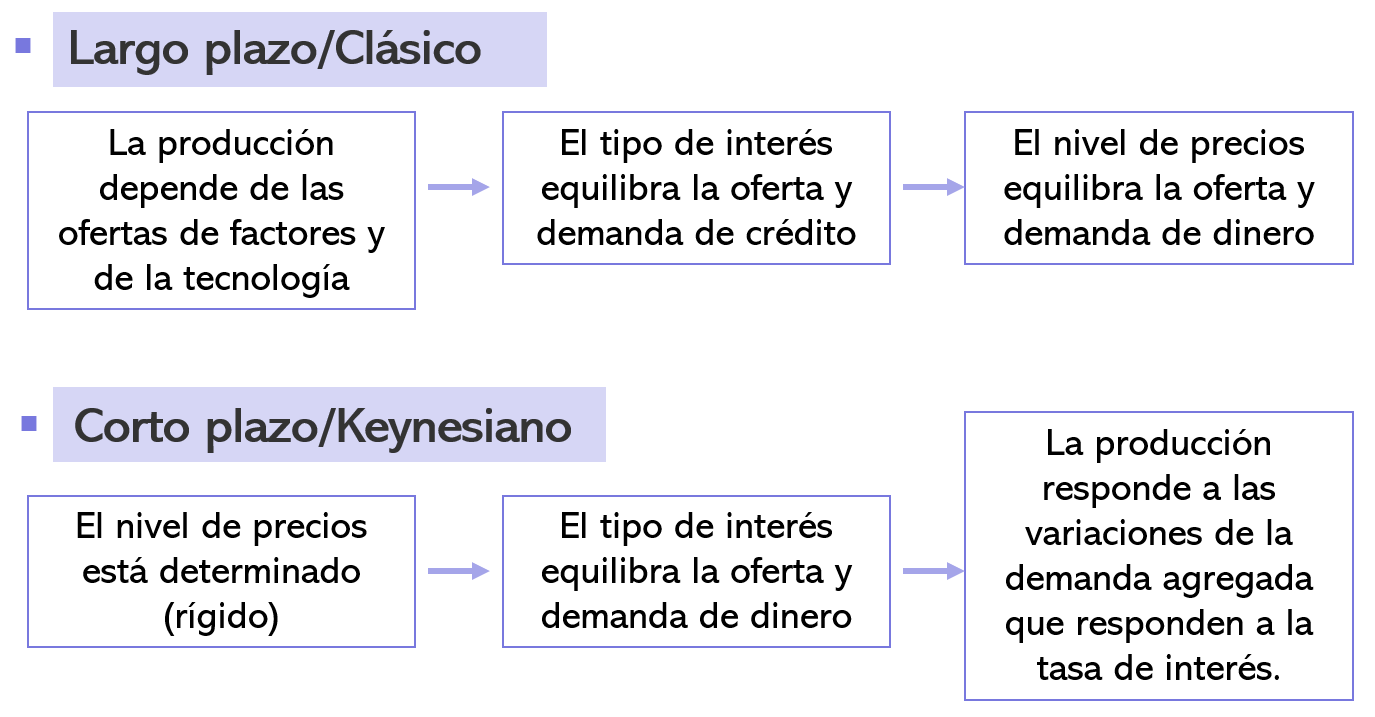
\includegraphics[width=11cm]{P18.png}\

\end{frame}

%---------------------------------------------------------------------------%

\begin{frame}{El enfoque Clásico y Keynesiano: Oferta Agregada}

\begin{itemize}
        \footnotesize\item La curva OA relaciona P (precios) con Y (producto).
        \footnotesize\item La forma de esta curva determina el mercado de trabajo.
\end{itemize}
\vspace{3mm}
\centering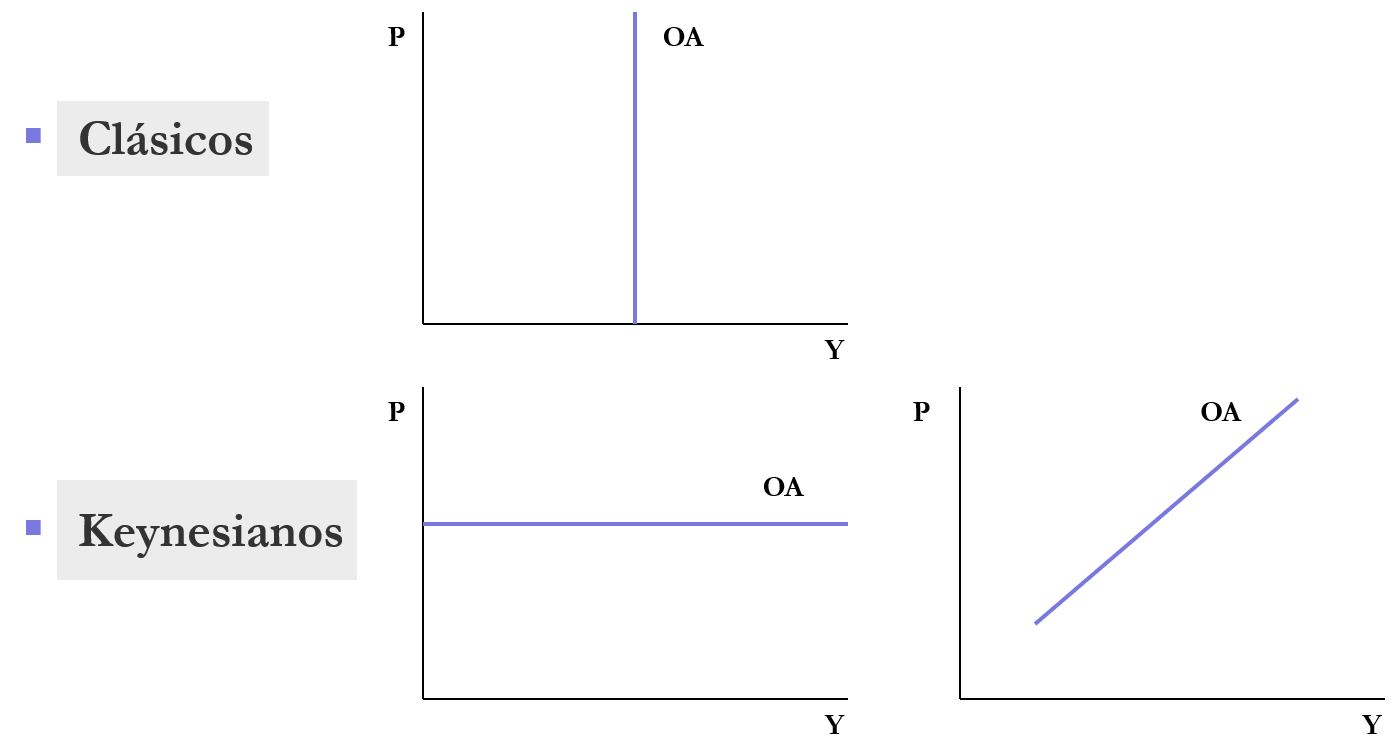
\includegraphics[width=10.5cm]{P19.png}\

\end{frame}

%---------------------------------------------------------------------------%

\begin{frame}{El enfoque Clásico y Keynesiano: Demanda Agregada}

\centering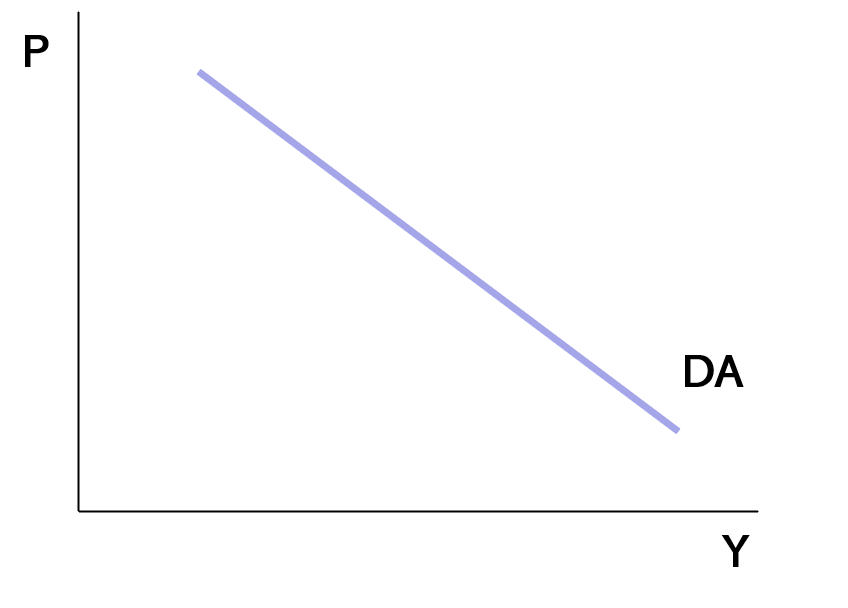
\includegraphics[width=6cm]{P20.png}\

    \begin{itemize}
        \item La forma de esta curva determina como C (consumo) e I (inversión) reaccionan frente al nivel de P (precios)
        \item El consumo y la inversión caen debido al incremento en los precios:
            \begin{itemize}
                \item Efecto riqueza
                \item Efecto tasa de interés: un aumento de P sin cambiar M lleva a tasas de interés más altas que hacen caer C e I.
            \end{itemize}
    \end{itemize}

\end{frame}

%---------------------------------------------------------------------------%

\begin{frame}{Shocks a la Demanda Agregada}
    
\centering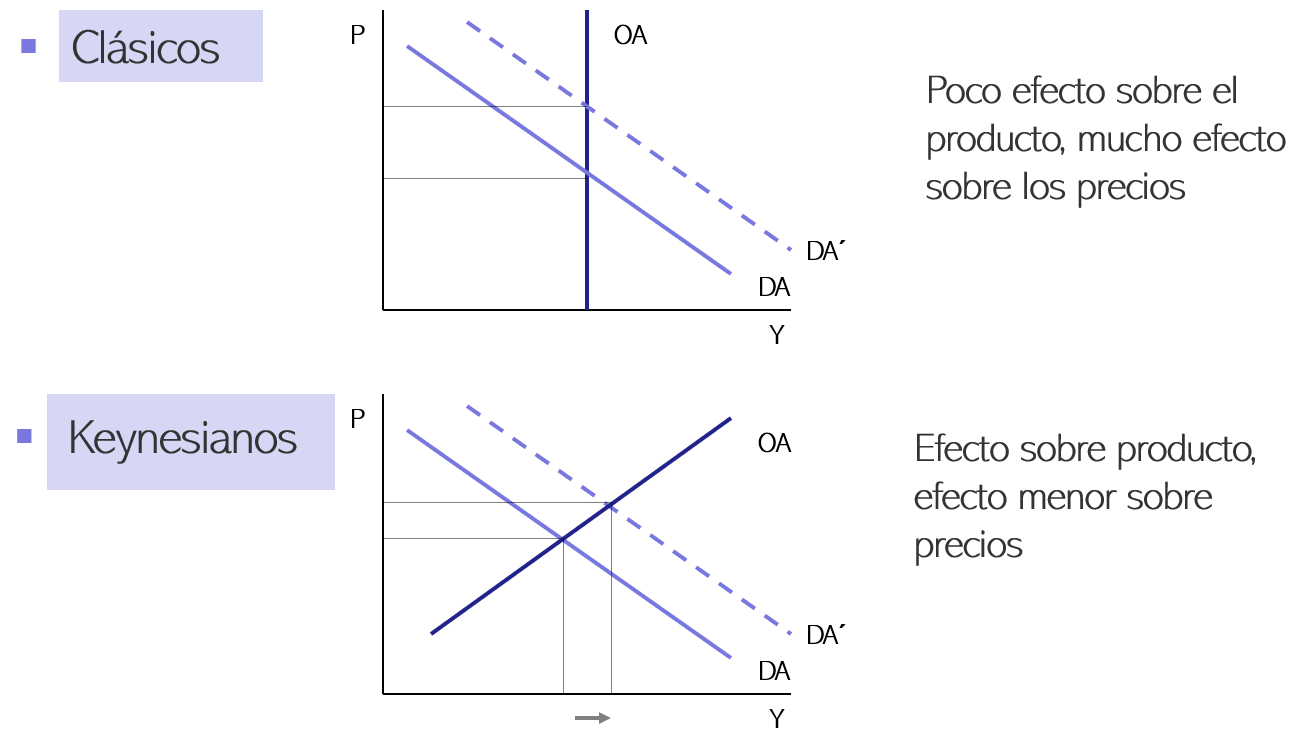
\includegraphics[width=12cm]{P21.png}\
    
\end{frame}

%---------------------------------------------------------------------------%

\begin{frame}{Shocks a la Oferta Agregada}

Los shocks de oferta negativos  producen un fenómeno que se conoce como estanflación

\begin{figure} [H]
\centering
\begin{minipage}{.5\textwidth}
  \centering
  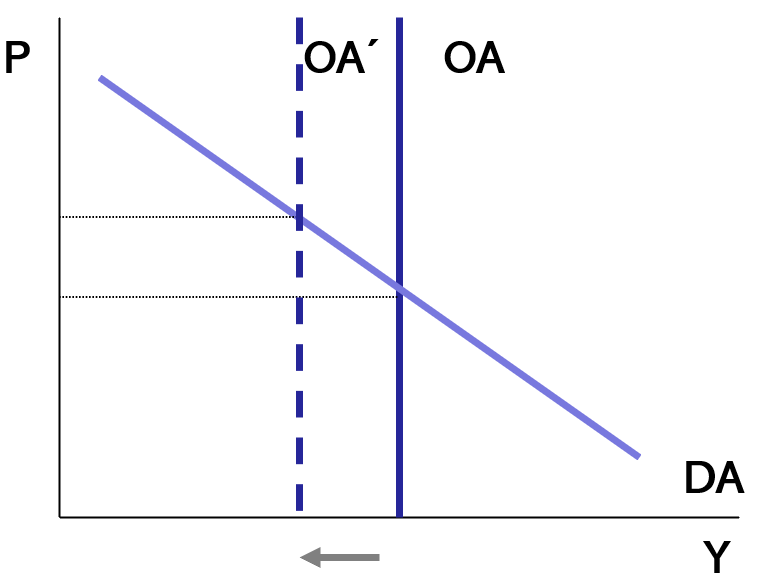
\includegraphics[width=0.9\textwidth]{P22_1.png}
  \caption{\textbf{Clásicos}}
  \label{a}
\end{minipage}%
\begin{minipage}{.5\textwidth}
  \centering
  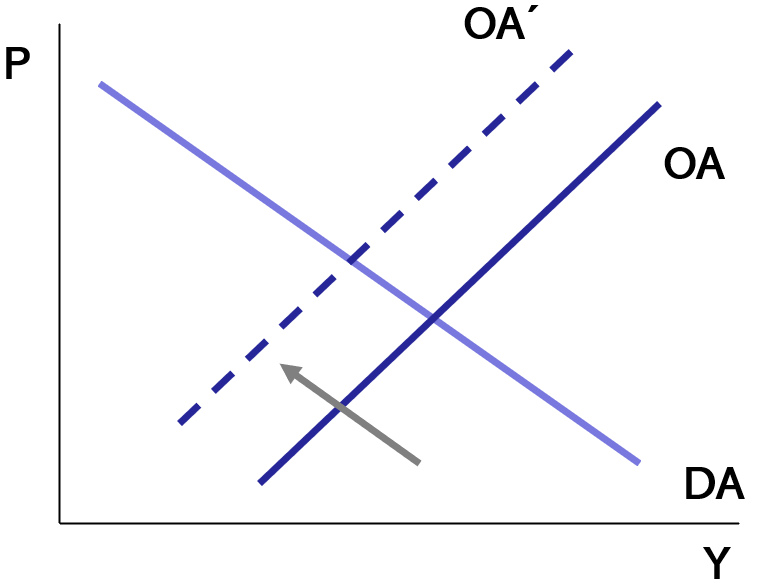
\includegraphics[width=0.9\textwidth]{P22_2.png}
  \caption{\textbf{Keynesianos}}
  \label{b}
\end{minipage}
\\
\end{figure}

\end{frame}

%---------------------------------------------------------------------------%

\begin{frame}{Ciclos: los Clásicos}

\begin{itemize}
    \item La explicación clásica de las fluctuaciones viene por cambios en la oferta agregada
\end{itemize}

\vspace{2mm}

\centering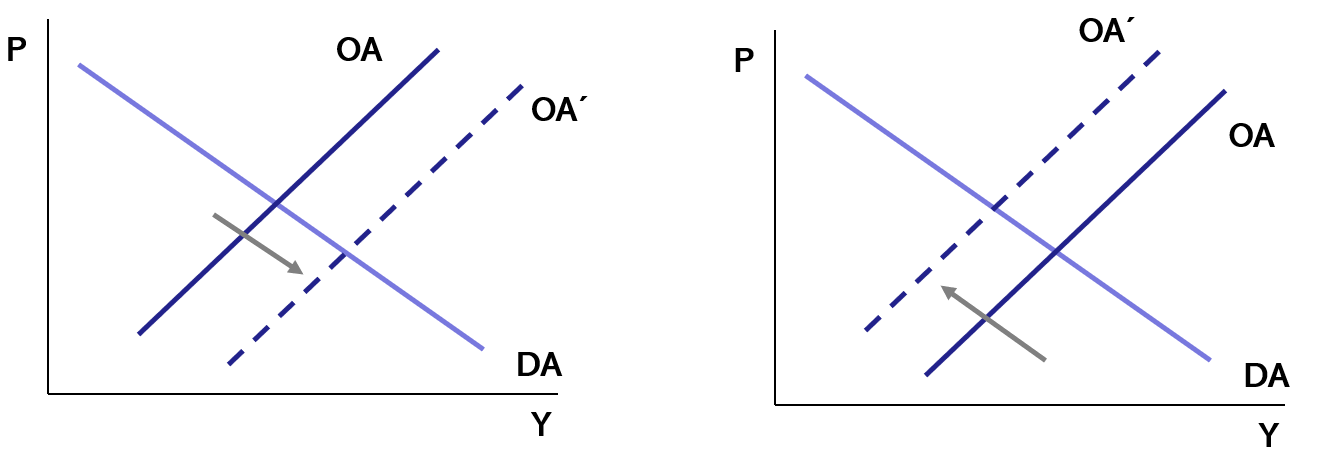
\includegraphics[width=12cm]{P23.png}\

\end{frame}

%---------------------------------------------------------------------------%

\begin{frame}{Ciclos: los Keynesianos}

\begin{itemize}
    \item La explicación keynesiana de las fluctuaciones viene por cambios en la demanda agregada
\end{itemize}

\vspace{2mm}

\centering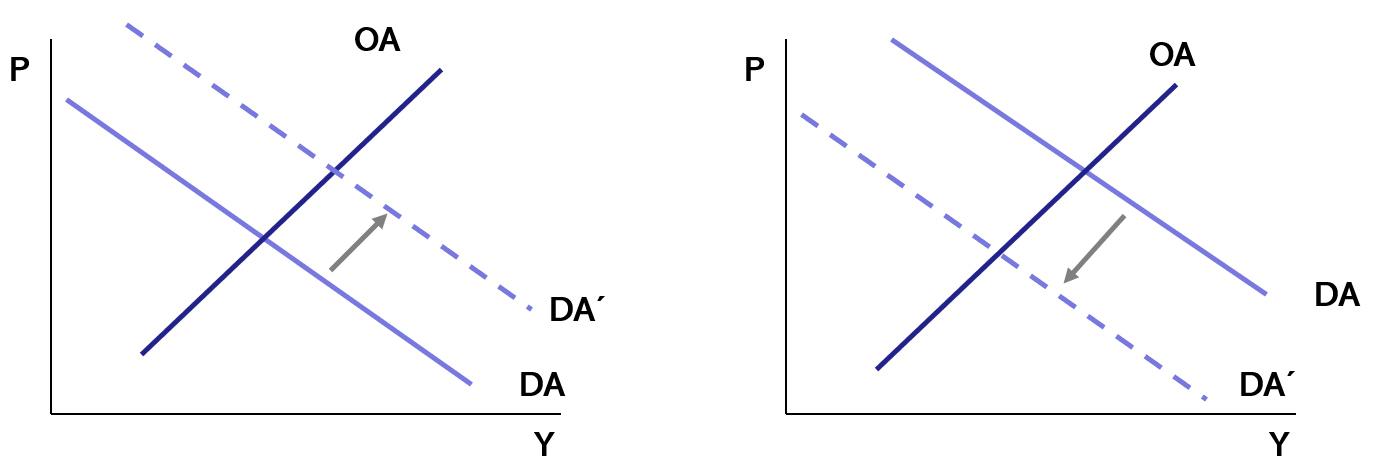
\includegraphics[width=12cm]{P24.png}\

\end{frame}

%---------------------------------------------------------------------------%
%---------------------------------------------------------------------------%

%\begin{frame}{}
%\centering 	\huge \textbf{El mercado de trabajo y la oferta %agregada} 
%\vspace{2mm}
%\hrule
%\end{frame}
%---------------------------------------------------------------------------%
%---------------------------------------------------------------------------%

%---------------------------------------------------------------------------%

%\begin{frame}{Mercado de trabajo: oferta de trabajo}

%\begin{itemize}
 %   \item ¿ Cómo responde la oferta de trabajo ante un cambio en los salarios?
  %  \vspace{2mm}
  %  \begin{itemize}
  %  \scriptsize\item Shock temporario $\Rightarrow$ la oferta de trabajo aumenta
  %  \scriptsize\item Shock permanente $\Rightarrow$ la oferta de trabajo no se modifica (mucho)
  % \scriptsize \item Un ejemplo que ilustra esto último: desde la época medieval hemos trabajado aprox unas 8 horas por día
 %   \end{itemize}
%\end{itemize}

%    \centering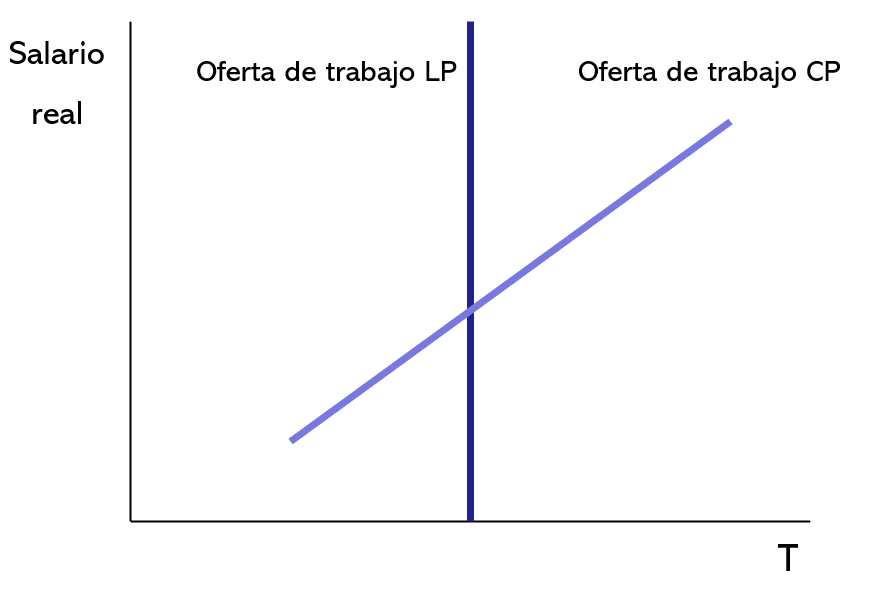
\includegraphics[width=8cm]{P26.png}\

%\end{frame}

%---------------------------------------------------------------------------%

%\begin{frame}{Mercado de trabajo: demanda de trabajo}

%\begin{itemize}
 %   \item Depende de los precios, productividad y ventas esperadas
%\end{itemize}

 %   \centering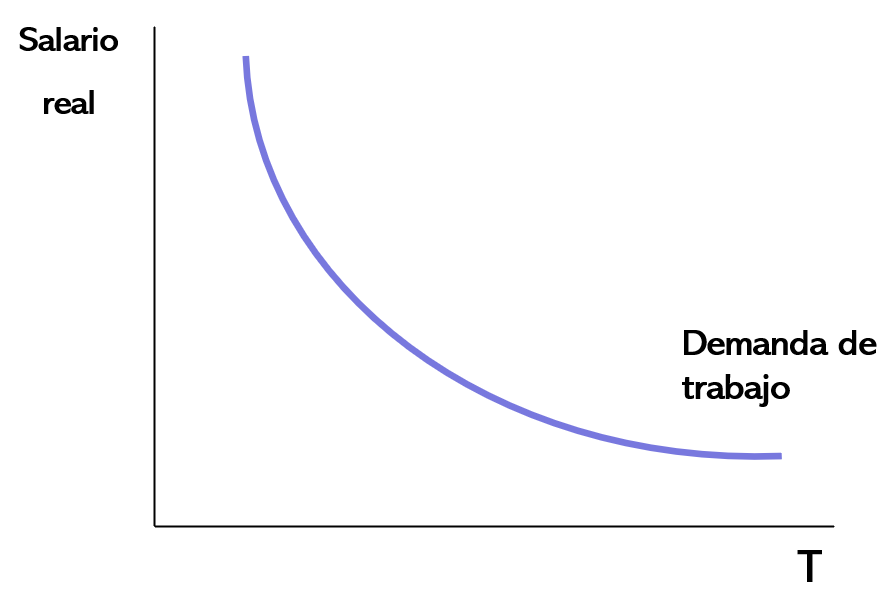
\includegraphics[width=9cm]{P27.png}\

%\end{frame}

%---------------------------------------------------------------------------%

\begin{frame}{Mercado de trabajo: equilibrio}

\begin{itemize}
    \item Si el salario está por encima de su valor de equilibrio (salario real*) habrá desempleo
\end{itemize}

    
\begin{center}
\begin{figure}[H]
\renewcommand{\figurename}{Figure}
\begin{center}
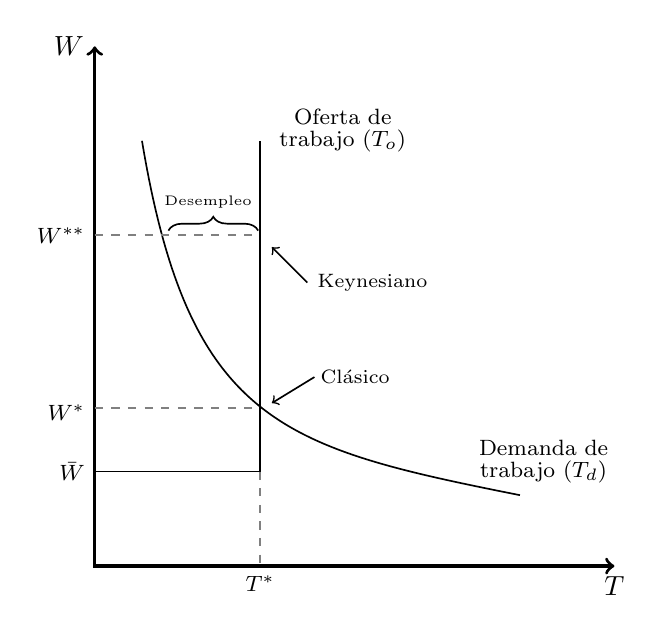
\begin{tikzpicture}[scale=0.6]
\draw[very thick,<->] (0,11) node[left]{$W$}--(0,0)--(11,0) node[below]{$T$};
\draw[semithick] (1,9).. controls (2,3) and (4, 2.5) .. (9, 1.5);
\node [] at (9.5,2.5) {\footnotesize Demanda de};
\node [] at (9.5,2) {\footnotesize trabajo ($T_d$)};
\draw[semithick](3.5,2)--(3.5,9);
\draw[thick, dashed, gray] (3.5,2)--(3.5,0);
\node [] at (5.25,9.5) {\footnotesize Oferta de};
\node [] at (5.25,9) {\footnotesize  trabajo ($T_o$)};
\node [below] at (3.5,0) {\footnotesize  $T^*$};
\node [left] at (0,3.25) {\footnotesize  $W^*$};
\draw[semithick, dashed,gray] (0,3.35)--(3.5,3.35);
\node [left] at (0,7) {\footnotesize  $W^{**}$};
\draw[semithick, dashed,gray] (0,7)--(3.5,7);
\draw (2.4,7.7) node[]{\tiny Desempleo};
\draw [semithick,decorate,decoration={brace,amplitude=5pt},xshift=-4pt,yshift=0pt](1.7,7.1) -- (3.6,7.1);
\node [left] at (0,2) {\footnotesize  $\bar{W}$}  ;
\draw[semithick] (0,2)--(3.5,2);
\node [left] at (7.25,6) {\scriptsize  Keynesiano}  ;
\node [left] at (6.45,4) {\scriptsize  Clásico}  ;
\draw[semithick, <-] (3.75,6.75)--(4.5,6);
\draw[semithick, <-] (3.75,3.45)--(4.65,4);
\end{tikzpicture}
\end{center}
\caption{\textbf{Equilibrio segun clásicos y keynesianos}}
\label{fig:C30.5}
\end{figure}
\end{center}  


\end{frame}



%---------------------------------------------------------------------------%

%\begin{frame}{La visión de los Clásicos}

%\begin{itemize}
%    \item Según esta visión el mercado de trabajo siempre está en equilibrio:
%    \vspace{2mm}
%    \begin{itemize}
%    \scriptsize\item Es decir que el salario real siempre iguala a %su valor de equilibrio (salario real*)
%    \scriptsize\item De esta manera, el nivel de actividad es siempre el de pleno empleo
%    \scriptsize \item Y la oferta agregada es vertical
%    \end{itemize}
%\end{itemize}

%    \centering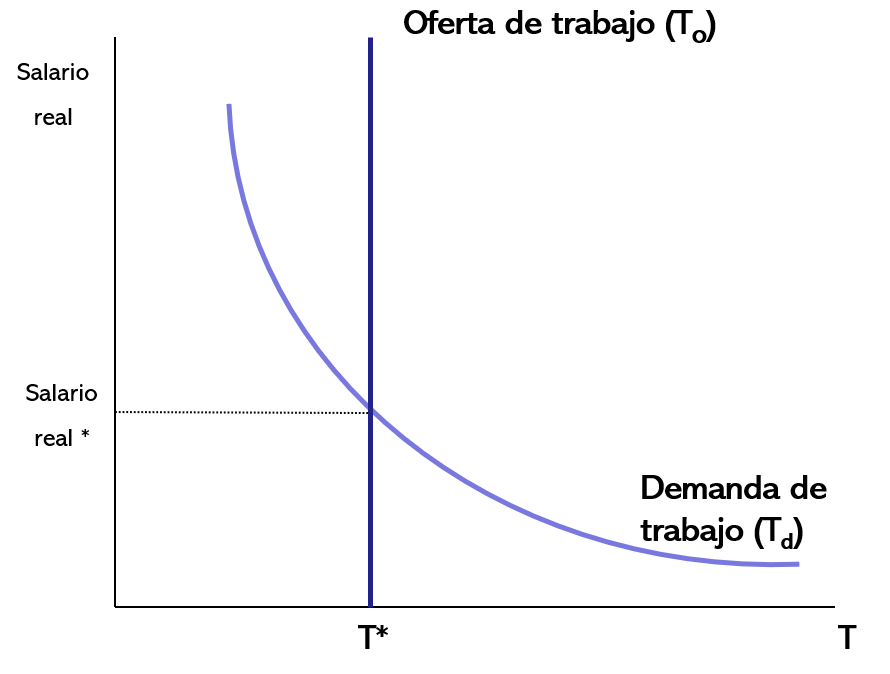
\includegraphics[width=8cm]{P29.png}\

%\end{frame}

%---------------------------------------------------------------------------%


\begin{frame}{La visión de los Clásicos}

    \centering
\includegraphics[width=5cm]{P29b.png}\

\begin{itemize}
    \item Desempleo Friccional
\item Salarios de reserva altos
\item Problemas de medición
   
\end{itemize}
\end{frame}
%---------------------------------------------------------------------------%
\begin{frame}{La visión Keynesiana}

\begin{itemize}
    \footnotesize\item El mercado de trabajo \textbf{no siempre} está en equilibrio:
    \vspace{2mm}
    \begin{itemize}
    \scriptsize\item ¿Por qué puede el salario real permanecer fuera del equilibrio?
    \begin{itemize}
        \scriptsize\item Rigideces nominales
        \scriptsize\item Sindicatos
        \scriptsize\item Contratos de largo plazo
        \scriptsize\item Salarios de eficiencia
       \end{itemize}
    \end{itemize}
\end{itemize}

    \centering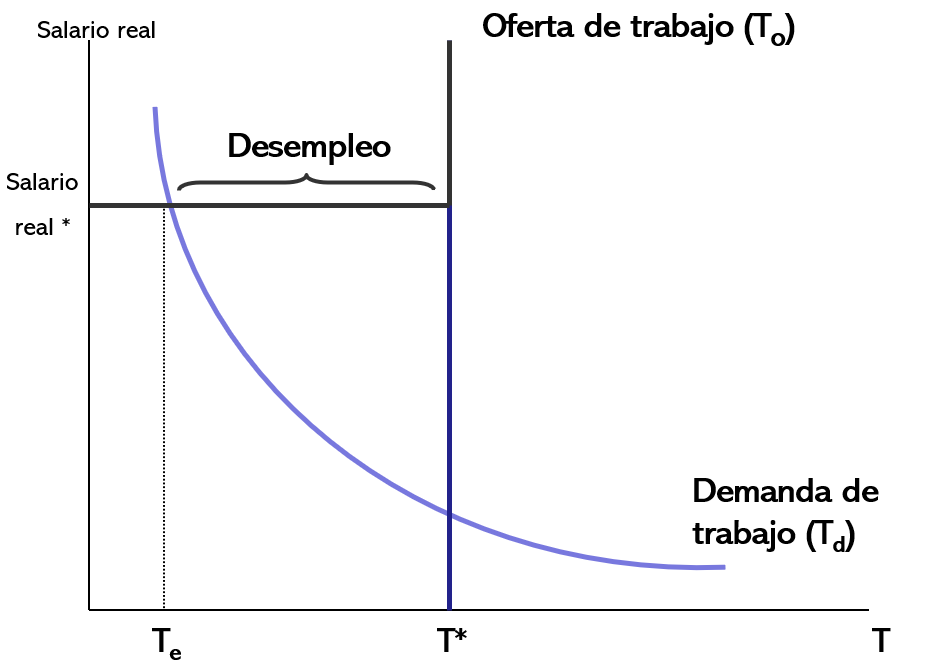
\includegraphics[width=8cm]{P30.png}\

\end{frame}

%---------------------------------------------------------------------------%

%\begin{frame}{La visión Keynesiana}

%\begin{itemize}
  %  \item Un aumento en la demanda por trabajo aumenta el nivel de actividad con un efecto reducido en salarios y precios.
  %  \item La oferta agregada se transforma, entonces, en horizontal
%\end{itemize}

%    \centering\includegraphics[width=8cm]{P31.png}\

%\end{frame}
%---------------------------------------------------------------------------%

\begin{frame}{¿Qué es el desempleo y cómo se mide?}

\begin{itemize}
    \item Desempleo involuntario: es el desempleo de la gente que busca pero no encuentra empleo
    \item Fuerza laboral: PEA (Población Económicamente activa)
        \begin{itemize}
            \item Empleados
            \item Desempleados
        \end{itemize}
\end{itemize}

\vspace{3mm}

\centering\includegraphics[width=6cm]{P32.png}\

\end{frame}

%---------------------------------------------------------------------------%

\begin{frame}{Indicadores básicos del mercado laboral}

\begin{itemize}
    \item Tasa de desempleo: $\frac{\text {Número de desempleados}}{\text{PEA}}$
    \vspace{3mm}
    \item \dangersignw Puede variar por: 
        \begin{itemize}
        \vspace{2mm}
            \scriptsize\item Cambios en el número de desempleados
            \vspace{2mm}
            \scriptsize\item Cambios en la fuerza laboral (PEA)
        \end{itemize}
    \vspace{3mm}
    \item Tasa de empleo $\frac{\text {Número de empleados}}{\text{Población}}$
    \vspace{3mm}
    \item Tasa de participación $\frac{\text {PEA}}{\text{Población}}$
\end{itemize}
 
\end{frame}

%---------------------------------------------------------------------------%

\begin{frame}{La tasa de desempleo en Argentina}

\centering\includegraphics[width=12cm]{P34.png}\

\end{frame}

%---------------------------------------------------------------------------%

\begin{frame}{Problemas con la serie de desempleo de INDEC}

\centering\includegraphics[width=12.5cm]{C30.15b.png}\

\end{frame}

%---------------------------------------------------------------------------%

\begin{frame}{El mercado de trabajo en la Argentina (1)}

\centering\includegraphics[width=12cm]{C30.16b.png}\

\end{frame}

%---------------------------------------------------------------------------%

\begin{frame}{El mercado de trabajo en la Argentina (2)}

\centering\includegraphics[width=12cm]{C30.17b.png}\

\end{frame}

%---------------------------------------------------------------------------%

%\begin{frame}{La tasa de desempleo en Argentina y EE.UU.}

%\centering\includegraphics[width=12cm]{P38.png}\

%\end{frame}

%---------------------------------------------------------------------------%

\begin{frame}{La recuperación de EE.UU. tardó en ocupar trabajo}

\centering\includegraphics[width=12cm]{P39.png}\

\end{frame}

%---------------------------------------------------------------------------%

%\begin{frame}{La recuperación de Argentina}

%\centering\includegraphics[width=12cm]{Recesiones.jpg}\

%\end{frame}

%---------------------------------------------------------------------------%

%\begin{frame}{El desempleo en los EE.UU.}

%\vspace{2mm}

%\centering\includegraphics[width=5.66cm]{NYT.png}\

%\end{frame}

%---------------------------------------------------------------------------%
%---------------------------------------------------------------------------%

\begin{frame}{}
\centering 	\huge \textbf{La demanda agregada y el mercado de crédito} 
\vspace{2mm}
\hrule
\end{frame}
%---------------------------------------------------------------------------%
%---------------------------------------------------------------------------%


%---------------------------------------------------------------------------%

\begin{frame}{Demanda Agregada}

    \begin{itemize}
\begin{tcolorbox}[width=4in,
                  interior hidden,
                  boxsep=0pt,
                  left=0pt,
                  right=0pt,
                  top=2pt,
                  ]%%
$$ Y = C + I + G $$
\end{tcolorbox}

    \end{itemize}
    
\centering donde C + I + G es la absorción.

\vspace{1cm}

 \begin{itemize}
        \item \textbf{C} depende de las expectativas, el ingreso disponible e impuestos
        \item \textbf{I} depende de las expectativas, impuestos y productividad
        \item Las dos se ven afectadas por la tasa de interés
    \end{itemize}

\end{frame}

%---------------------------------------------------------------------------%

\begin{frame}{¿Cómo se determina el consumo?}
    \begin{itemize}
        \item Depende del ingreso actual y el esperado
        \item La teoría básica del consumo es la de la “suavización del consumo” a lo largo de la vida
        \item Lo que implica que 
            \begin{itemize}
            \item Ante cambios temporarios en el ingreso:
                \begin{itemize}
                \item Hay pequeños cambios en el consumo (y mucho cambio en el ahorro)
                \end{itemize}            
            \item Ante cambios permanentes en el ingreso:
                \begin{itemize}
                \item Hay grandes cambios en el consumo actual (y poco cambio en el ahorro)
                \end{itemize}
            \end{itemize}
        \item El consumo cambia más ante cambios en las expectativas que ante cambios reales!!!
        \item Pero la tasa de interès tambièn lo afecta alterando el deseo de "consumo hoy" vs "consumo mañana"
    \end{itemize}
\end{frame}

%---------------------------------------------------------------------------%
\begin{frame}{La suavización del consumo gráficamente}

\begin{center}
\begin{figure}[h!]
\renewcommand{\figurename}{Figure}
\begin{center}
    \begin{minipage}[b]{0.45\textwidth}
        \begin{center}
\begin{tikzpicture}[scale=0.4]
\draw[very thick,<->] (0,11) node[left]{$C,Y$}--(0,0)--(11,0) node[below]{$t$};

\draw[semithick, gray](0, 4)--(3, 4)--(3,6)--(8.5,6) node[right] {\scriptsize $Y=C$};
\draw[thick, dashed, red](0, 4)--(3, 4)--(3,6)--(8.5,6);
\draw[thick, dotted](3,4)--(3,0) node [below] {\footnotesize $t_0$};
\end{tikzpicture}
\end{center}
     \end{minipage}
  %  \hfill
    \begin{minipage}[b]{0.45\textwidth}
    \begin{center}
\begin{tikzpicture}[scale=0.4]
\draw[very thick,<->] (0,11) node[left]{$C,Y$}--(0,0)--(11,0) node[below]{$t$};
\draw[semithick, gray](0, 4)--(3, 4)--(3,6)--(5,6)--(5,4)--(8.5,4)node[right] {\scriptsize $Y$};
\draw[thick, dashed, red](0, 4)--(3, 4)--(3,5)--(8.5,5) node[right] {\scriptsize $C$};
\draw[thick, dotted](3,4)--(3,0) node [below] {\footnotesize $t_0$};
%\draw[thick, dashed](0, 4)--(3,4)--(3,6)--(5,6);
\end{tikzpicture}
\end{center}
    \end{minipage}
\end{center}
\caption{\textbf{Suavización del consumo}}
\label{fig:31.1}
\end{figure}
\end{center}


\end{frame}

%---------------------------------------------------------------------------%


%\begin{frame}{La suavización del consumo en gráficos}
%    \begin{center}
%\begin{figure}[H]
%\renewcommand{\figurename}{Figure}
%\begin{center}
%\begin{tikzpicture}[scale=0.6]
%\draw[very thick,<->] (0,11) node[left]{$c_{t+1}$}--(0,0)--(11,0) node[below]{$c_{t}$};
%\draw[semithick] (0,7)--(8,0);
% \draw[thick,gray, dashed](3.5, 3.95)--(3.5, 0);
%  \draw[thick,gray, dashed](3.5, 3.95)--(0, 3.95);
% \node[below] at (3.5,0) {\footnotesize $y_t$};
%  \node[left] at (0,3.95) {\footnotesize $y_{t+1}$};
%  \draw[fill] (3.5,3.95) circle [radius =0.11] ;
%\end{tikzpicture}
%\end{center}
%\caption{\textbf{Restricción intertemporal}}
%\label{fig:C31.3}
%\end{figure}
%\end{center} 
%\end{frame}



%\begin{frame}{La suavización del consumo en gráficos}
%\begin{center}
%\begin{figure}[H]
%\renewcommand{\figurename}{Figure}
%\begin{center}
%\begin{tikzpicture}[scale=0.6]
%\draw[very thick,<->] (0,11) node[left]{$c_{t+1}$}--(0,0)--(11,0) node[below]{$c_{t}$};
%\draw[semithick] (2,8).. controls (2.5,2.5) and (4,1) ..(8,0);
%\draw[semithick] (2,8).. controls (2.5,2.5) and (4,0.75) ..(8.25,0.65);
% \draw[thick,gray, dashed](2.15, 7)--(2.85, 4);
%   \draw[fill] (2.1,7) circle [radius =0.11] ;
% \draw[thick,gray, dashed](4.2, 1.9)--(2.85, 4);      
%      \draw[fill] (2.8,3.95) circle [radius =0.11] ;
%\draw[fill] (4.2,1.8) circle [radius =0.11] ;      
%\draw[semithick, ->] (2.1,7)--(2.1,4);
%\draw[semithick, ->] (2.1,3.95)--(2.7,3.95);
%\draw[semithick, ->] (2.8,3.95)--(2.8,1.8);
%\draw[semithick, ->] (2.85,1.8)--(4,1.8);
%\end{tikzpicture}
%\end{center}
%\caption{\textbf{Curva de indiferencia}}
%\label{fig:C31.4}
%\end{figure}
%\end{center}  
%\end{frame}

%\begin{frame}{La suavización del consumo en gráficos}

%\begin{center}
%\begin{figure}[H]
%\renewcommand{\figurename}{Figure}
%\begin{center}
%\begin{tikzpicture}[scale=0.6]
%\draw[very thick,<->] (0,11) node[left]{$c_{t+1}$}--(0,0)--(11,0) node[below]{$c_{t}$};
%\draw[semithick, gray] (1,9).. controls (2,3) and (4, 2.5) .. (9, 1.5) ;
%\draw[semithick, gray] (2,9).. controls (2.5,3.75) and (6.8, 3) .. (8.8, 2.5);
%\draw[semithick] (2.25,9).. controls (2.75,4) and (7, 3) .. (9, 2.75);
%\draw[semithick] (0,8.75)--(9.1,0);
% \draw[thick,gray, dashed](4.1, 4.65)--(4.1, 0);
% \draw[thick,gray, dashed](4.1, 4.85)--(0, 4.85);
% \draw[fill] (4.1,4.85) circle [radius =0.11] ;  
% \node[below] at (4.1,0) {\footnotesize $c_t$};
% \node[left] at (0,4.85){\footnotesize $c_{t+1}$};
% \draw[thick,gray, dashed](2.95, 5.925)--(2.95, 0);
% \draw[thick,gray, dashed](2.95, 5.925)--(0, 5.925);
% \draw[fill] (2.95,5.925) circle [radius =0.11] ;   
% \node[below] at (2.95,0) {\footnotesize $y_t$};
% \node[left] at (0,5.925){\footnotesize $y_{t+1}$};
% \node [right] at (5.1,5.75) {\scriptsize  Equilibrio}  ;
%\draw[semithick, <-] (4.3,4.95)--(5.2,5.5);
%\draw [semithick,decorate,decoration={brace,amplitude=3pt,mirror},xshift=5pt,yshift=0pt](2.75,-0.6) -- (3.9,-0.6);
%\draw (3,-1) node[]{\tiny Consumidor pide};
%\draw (2.55,-1.25) node[]{\tiny prestado...};
%\draw [semithick,decorate,decoration={brace,amplitude=3pt,mirror},xshift=0pt,yshift=5pt](-1.25,5.85) -- (-1.25,4.7);
%\draw (-2.25,5.5) node[]{\tiny ... y};
%\draw (-2.25,5.25) node[]{\tiny devuelve};
%\end{tikzpicture}
%\end{center}
%\caption{\textbf{Equilibrio}}
%\label{fig:C31.5}
%\end{figure}
%\end{center}  
%\end{frame}


\begin{frame}{El efecto tasa de interes}


\begin{center}
\begin{figure}[H]
\renewcommand{\figurename}{Figure}
\begin{center}
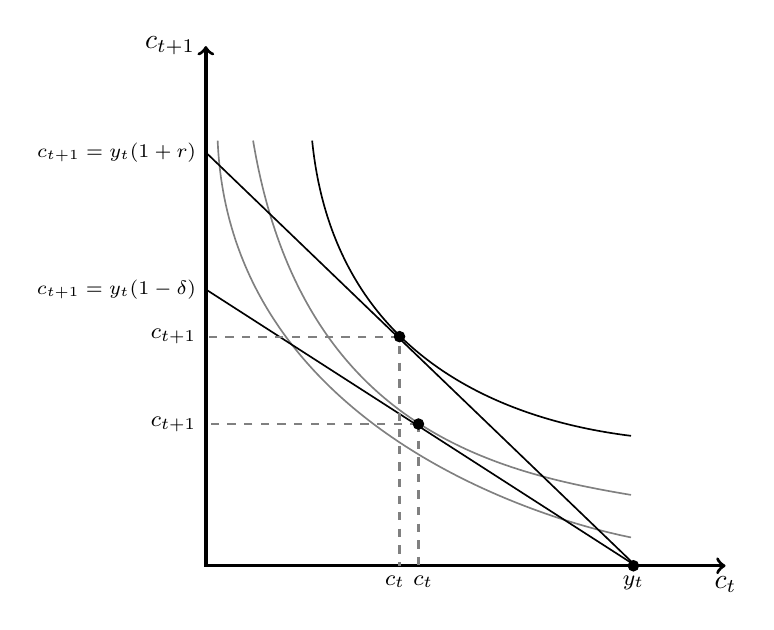
\begin{tikzpicture}[scale=0.6]
\draw[very thick,<->] (0,11) node[left]{$c_{t+1}$}--(0,0)--(11,0) node[below]{$c_{t}$};
\draw[semithick, gray] (1,9).. controls (2,3) and (6, 2) .. (9, 1.5) ;
%\draw[semithick, gray] (0.25,9).. controls (0.5,3) and (7, 1) .. (9, 0);
\draw[semithick, gray] (0.25,9).. controls (0.5,3) and (7, 1) .. (9, 0.6);
\draw[semithick] (2.25,9).. controls (2.75,4) and (7, 3) .. (9, 2.75);
\draw[semithick] (0,8.75)--(9.1,0);
\draw[semithick] (0,5.85)--(9.1,0);
  \draw[thick,gray, dashed](4.1, 4.65)--(4.1, 0);
  \draw[thick,gray, dashed](4.1, 4.85)--(0, 4.85);
  \draw[fill] (4.1,4.85) circle [radius =0.11] ;  
  \node[below] at (4,0) {\footnotesize $c_t$};
  \node[left] at (0,4.85){\footnotesize $c_{t+1}$};
%  \draw[thick,gray, dashed](2.95, 5.925)--(2.95, 0);
%  \draw[thick,gray, dashed](2.95, 5.925)--(0, 5.925);
  \draw[thick,gray, dashed](4.5, 3)--(4.5, 0);
  \draw[thick,gray, dashed](4.5, 3)--(0, 3);
  \node[below] at (4.6,0) {\footnotesize $c_t$};
  \node[left] at (0,3){\footnotesize $c_{t+1}$};
  \draw[fill] (4.5,3) circle [radius =0.11] ;   
    \draw[fill] (9.05,0) circle [radius =0.11] node [below] {\footnotesize $y_t$} ;   
  \node[left] at (0,5.85){\scriptsize $c_{t+1} = y_t (1-\delta)$};   
  \node[left] at (0,8.75){\scriptsize $c_{t+1} = y_t (1+r)$};
\end{tikzpicture}
\end{center}
\caption{\textbf{Efecto de la tasa de interés}}
\label{fig:C31.6}
\end{figure}
\end{center}  
\end{frame}



\begin{frame}{El Gran Elon}
   \begin{figure} [H]
    \centering
    \href{https://twitter.com/Stelladmarco/status/1103059259586052097}{
    \includegraphics[scale=0.5]{images/C31.9.png}}
\end{figure} 
\end{frame} 

\begin{frame}{Apalancamiento}
   \begin{center}
\begin{figure}[H]
\renewcommand{\figurename}{Figure}
\begin{center}
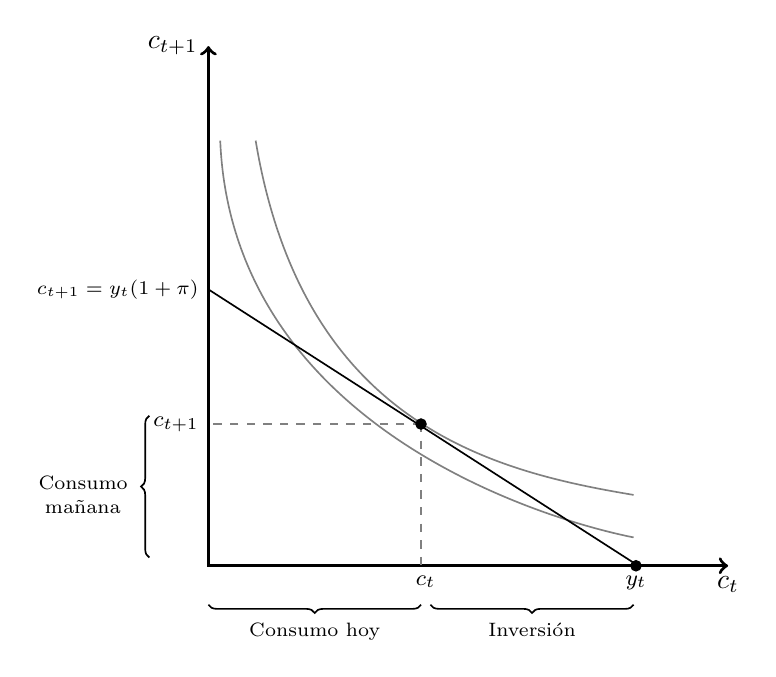
\begin{tikzpicture}[scale=0.6]
\draw[very thick,<->] (0,11) node[left]{$c_{t+1}$}--(0,0)--(11,0) node[below]{$c_{t}$};
\draw[semithick, gray] (1,9).. controls (2,3) and (6, 2) .. (9, 1.5) ;
%\draw[semithick, gray] (0.25,9).. controls (0.5,3) and (7, 1) .. (9, 0);
\draw[semithick, gray] (0.25,9).. controls (0.5,3) and (7, 1) .. (9, 0.6);
\draw[semithick] (0,5.85)--(9.1,0);
  \draw[thick,gray, dashed](4.5, 3)--(4.5, 0);
  \draw[thick,gray, dashed](4.5, 3)--(0, 3);
  \node[below] at (4.6,0) {\footnotesize $c_t$};
  \node[left] at (0,3){\footnotesize $c_{t+1}$};
  \draw[fill] (4.5,3) circle [radius =0.11] ;   
    \draw[fill] (9.05,0) circle [radius =0.11] node [below] {\footnotesize $y_t$} ;   
  \node[left] at (0,5.85){\scriptsize $c_{t+1} = y_t (1+\pi)$};   
 \draw [semithick,decorate,decoration={brace,amplitude=3pt},xshift=0pt,yshift=5pt](-1.25,0) -- (-1.25,3);  
  \draw [semithick,decorate,decoration={brace,amplitude=3pt, mirror},xshift=0pt,yshift=5pt](0,-1) -- (4.5,-1); 
  
    \draw [semithick,decorate,decoration={brace,amplitude=3pt, mirror},xshift=0pt,yshift=5pt](4.7,-1) -- (9,-1); 
  \node[left] at (-1.5,1.75){\scriptsize Consumo};   
    \node[left] at (-1.65,1.25){\scriptsize mañana};
  \node[below] at (2.25,-1){\scriptsize Consumo hoy};      
    \node[below] at (6.85,-1){\scriptsize Inversión};     
\end{tikzpicture}
\end{center}
\caption{\textbf{Efecto de la tasa de interés}}
\label{fig:C31.7}
\end{figure}
\end{center}   
\end{frame}






\begin{frame}{Apalancamiento}
    \begin{center}
\begin{figure}[H]
\renewcommand{\figurename}{Figure}
\begin{center}
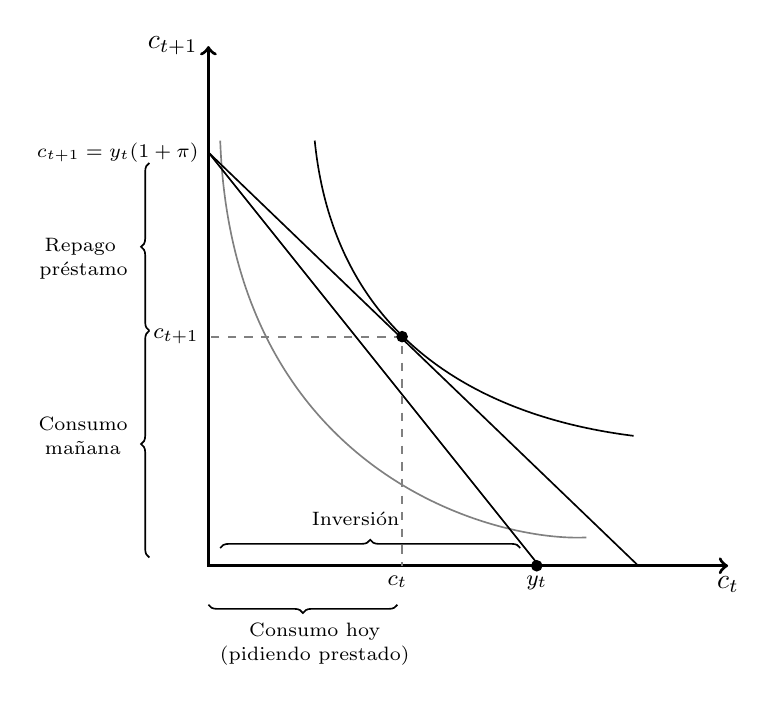
\begin{tikzpicture}[scale=0.6]
\draw[very thick,<->] (0,11) node[left]{$c_{t+1}$}--(0,0)--(11,0) node[below]{$c_{t}$};
%\draw[semithick, gray] (0.25,9).. controls (0.5,2) and (6, 0.5) .. (7, 0);
\draw[semithick, gray] (0.25,9).. controls (0.5,2) and (6, 0.5) .. (8, 0.6);
\draw[semithick] (2.25,9).. controls (2.75,4) and (7, 3) .. (9, 2.75);
\draw[semithick] (0,8.75)--(9.1,0);
\draw[semithick] (0,8.75)--(7,0);
  \draw[thick,gray, dashed](4.1, 4.65)--(4.1, 0);
  \draw[thick,gray, dashed](4.1, 4.85)--(0, 4.85);
  \draw[fill] (4.1,4.85) circle [radius =0.11] ;  
  \node[below] at (4,0) {\footnotesize $c_t$};
  \node[left] at (0,4.85){\footnotesize $c_{t+1}$};
    \draw[fill] (6.95,0) circle [radius =0.11] node [below] {\footnotesize $y_t$} ;   
  \node[left] at (0,8.75){\scriptsize $c_{t+1} = y_t (1+\pi)$}; 
   \draw [semithick,decorate,decoration={brace,amplitude=3pt},xshift=0pt,yshift=5pt](-1.25,0) -- (-1.25,4.8); 
      \draw [semithick,decorate,decoration={brace,amplitude=3pt,mirror},xshift=0pt,yshift=5pt](-1.25,8.35) -- (-1.25,4.8); 
  \draw [semithick,decorate,decoration={brace,amplitude=3pt, mirror},xshift=0pt,yshift=5pt](0,-1) -- (4,-1); 
\draw [semithick,decorate,decoration={brace,amplitude=3pt},xshift=0pt,yshift=5pt](0.25,0.2) -- (6.6,0.2); 
  \node[left] at (-1.5,3){\scriptsize Consumo};   
    \node[left] at (-1.65,2.5){\scriptsize mañana};
  \node[below] at (2.25,-1){\scriptsize Consumo hoy};
  \node[below] at (2.25,-1.5){\scriptsize (pidiendo prestado)};
    \node[left] at (4.25,1){\scriptsize Inversión};
      \node[left] at (-1.75,6.75){\scriptsize Repago };   
    \node[left] at (-1.5,6.25){\scriptsize préstamo};
\end{tikzpicture}
\end{center}
\caption{\textbf{Efecto de la tasa de interés}}
\label{fig:C31.8}
\end{figure}
\end{center} 
\end{frame}

 
\begin{frame}{Otras teorías del ahorro}
   \begin{itemize}
       \item Ciclo de vida
       \item Hipotecas revertidas
       \item Los tests de Shea
       \item Ahorro precautorio
       \item La fuerza de los defaults
       \item Present bias
       \item Ubank...
   \end{itemize} 
\end{frame}


\begin{frame}{La inversion: valor presente}
    \begin{equation}
VPN = \sum_{t=0} ^{T} \frac{1}{(1+r)^t} W_t,
\end{equation}

\begin{itemize}
    \item $r$ es el costo del capital 
    \item Si el VPN$>0$, entonces convendría invertir
    \item Si VPN $<0$ no convendría
\end{itemize}

 
\end{frame}




\begin{frame}{El WACC}
\begin{itemize}
    \item  ¿Cual es el costo de capital que deberíamos usar?
    \item La manera mas conocida es la del costo capital promedio ponderado (CCPP, o WACC por sus siglas en inglés)
\end{itemize}
     
\begin{equation}
WACC=\alpha _{eq}r_{eq}+\left( 1-\alpha _{eq}\right) r_{debt},
\end{equation}

\begin{equation}
\alpha _{eq}=\left( \frac{\text{Net worth}}{\text{Total Assets}}\right) .
\end{equation}
\end{frame}

%\begin{frame}{La opción de invertir de Pindyck}
%    Supongamos que podemos hacer una inversión inicial de \$2200, lo que nos lleva al siguiente pago estocástico:
%    \begin{center}
%\begin{tabular}{cccc}
%\begin{array}{cccc}
%t=0 & & t=1& \hspace{0.15cm} t=2\\[1.5mm]
%& q &P_{1} = 300&\hspace{0.15cm}... \\
%P_{0}=200&&&\\
%&1-q&P_{1} = 100&\hspace{0.15cm} ...  \\
%\end{array}
%\end{tabular}
%\end{center}
%\end{frame}


%\begin{frame}{La opción de invertir de Pindyck}
%    \begin{equation}
%VPN= - 2200+\sum\limits_{t=0}^{\infty }\frac{200}{\left( 1.1\right) ^{t}}%
%=-2200+2200=\$0.  \label{basic}
%\end{equation}

%\end{frame}

%\begin{frame}{La opción de invertir de Pindyck}
%Que pasa si espero un periodo para invertir?
%\scriptsize
%\begin{equation}
%VPN=0.5\left[ -\frac{2200}{1.1}+\sum\limits_{t=1}^{\infty }\frac{300}{%
%\left( 1.1\right) ^{t}}\right] =0.5\left[ -\frac{2200}{1.1}+\frac{300}{%
%\left( 1.1\right) }\left( 1+\frac{1}{1.1}+\frac{1}{1.1^{2}}+ ... \right) %
%\right]
%\end{equation}

%\begin{equation}
%=0.5\left[ -\frac{2200}{1.1}+\frac{300}{\left( 1.1\right) }\left( \frac{1%
%}{1-\frac{1}{1.1}}\right) \right] =0.5\left[ -\frac{2200}%{1.1}+\frac{300}{
%\left( 1.1\right) }\left( \frac{1.1}{0.1}\right) \right] = 500!
%\end{equation}

%\end{frame}






\begin{frame}{Demanda agregada y el mercado de crédito}

    \begin{itemize}
\begin{tcolorbox}[width=4in,
                  interior hidden,
                  boxsep=0pt,
                  left=0pt,
                  right=0pt,
                  top=2pt,
                  ]%%
$$ Y = C(r) + I(r) + G $$
\end{tcolorbox}
    \end{itemize}
    
\centering \small{(donde r es la tasa de interés real)}.

 \begin{itemize}
        \item En una economía cerrada:
        
        \begin{tcolorbox}[width=4in,
                  interior hidden,
                  boxsep=0pt,
                  left=0pt,
                  right=0pt,
                  top=2pt,
                  ]%%
                    $$ Y – C – G = I $$
        \end{tcolorbox}
        
    \end{itemize}
    
     \begin{itemize}
        \item Que es como decir que lo que ahorro es lo que invierto
        \item Y esto determina la tasa de interés real
        \item Los ahorros son intermediados por el sector financiero hacia inversiones reales
        \item Economías que ahorran mucho invierten mucho (China, Japón), economías que ahorran poco invierten menos (Brasil, Argentina)! 
    \end{itemize}
 


\end{frame}

%---------------------------------------------------------------------------%

%\begin{frame}{El mercado de crédito}

%\centering\includegraphics[width=6.5cm]{P46.png}\


%    \begin{itemize}
%        \item La oferta la define el deseo de la gente de ahorrar
%        \item La oferta de fondos depende de la tasa de interés
%        \item La demanda viene dada por la inversión o la demanda de deuda de parte del gobierno
%        \item Ambas decrecen con la tasa de interés
%    \end{itemize}

%\end{frame}




%---------------------------------------------------------------------------%
%---------------------------------------------------------------------------%

\begin{frame}{}
\centering 	\huge \textbf{El mercado monetario} 
\vspace{2mm}
\hrule
\end{frame}
%---------------------------------------------------------------------------%
%---------------------------------------------------------------------------%

\begin{frame}{El dinero:funciones}
    \begin{itemize}
   
    \item \textbf{Medio de cambio}: El dinero es utilizado como un mecanismo para realizar transacciones. 
  
    \item \textbf{Unidad de cuenta}: El dinero es también una medida que sirve para definir precios así como para registrar activos y deudas.
    
    \item \textbf{Depósito de valor}: El dinero permite transferir poder adquisitivo del presente al futuro. 
    
\end{itemize}
\end{frame}


\begin{frame}{Tipos de dinero}
    \begin{itemize}
        \item Commodity money 
        \begin{figure} [H]   
  \centering
  \includegraphics[width=.8\textwidth]{images/C32.1.jpg}
      \caption{Monedas carcomidas}
  \label{fig:C32.1}
\end{figure}
   
    \end{itemize}
\end{frame}

\begin{frame}{Dinero Papel}
    \begin{itemize}
        \item Comienza a usarse en China en siglo VII
        \item Antes de los bancos centrales los emitían los bancos 
        
        
\begin{figure} [H]   
  \centering
  \includegraphics[width=.4\textwidth]{images/C32.2.jpg}
      \caption{Dollar de Bank of Rahway, New Jersey, 1850. Via Wikimedia Commons}
  \label{fig:C32.2}
\end{figure}

\begin{figure} [H]   
  \centering
  \includegraphics[width=.4\textwidth]{images/C32.3.jpeg}
      \caption{Detroit City Bank \$3 Note}
  \label{fig:C32.3}
\end{figure}
\end{itemize}
\end{frame}
        
\begin{frame}{Dinero }
        \begin{figure} [H]   
  \centering
  \includegraphics[width=.35\textwidth]{images/C32.4.jpg}
      \caption{Billetes emitidos por el Banco Provincia de Buenos Aires}
  \label{fig:C32.4}
\end{figure}

\begin{figure} [H]   
\centering\includegraphics[width=.38\textwidth]{images/C32.5.jpg}
\caption{Billetes emitidos por el Banco Provincia de Buenos Aires}
\end{figure}
       \begin{itemize}
           \item  Luego lo monopolizaron los bancos centrales
    \item Y hoy volvemos a la multiplicidad de monedas 
       \end{itemize}     
        \end{frame}
        

\begin{frame}{¿Qué más hace el Banco Central?}
    \begin{itemize}
    \item Crea y regula la cantidad de dinero en la economía 
    \item Regula la actividad bancaria
    \item Es prestamista de última instancia
    \item Maneja la política cambiaria 
    
\end{itemize}
\end{frame}

\begin{frame}{¿Qué son los bancos?}
    \begin{itemize}
    \item Intermedian entre depositantes y tomadores de crédito
    \item Son parte del proceso de creación de dinero
    \item Hacen una transformaci'on de madurez: por eso decimos que crean tiempo
    \item Diversifican el riesgo de la cartera de inversión
    \begin{center}
       $ spread = {\text{tasa activa}} - {\text{tasa pasiva}}  $
    \end{center}
     
    
\end{itemize}
\end{frame}


\begin{frame}{Riesgos que tienen que manejar los bancos}

\begin{itemize}
    \item \textbf{Riesgo de madurez}: Como el banco invierte en activos de largo plazo, si la tasa de interés sube, en general el valor de los activos de largo plazo va a caer más que los de corto plazo. 
    \item \textbf{Riesgo de liquidez}: Es el riesgo de que el activo no se pueda transformar en efectivo (liquidar) sin generar una pérdida financiera. 
    \item \textbf{Riesgo de default}: Es el riesgo de que los créditos del banco no sean repagados.
\end{itemize}
    




\end{frame}


\begin{frame}{Aplancamiento (leverage)}
    \begin{center}
       $ Leverage = \frac{Activo}{\text{Patrimonio Neto}}. $
    \end{center} 
    


    
    
\end{frame}

\begin{frame}{Apalancamiento II}
    \begin{table}[H]
    \centering

%    \vspace{.3cm}
    %\scalebox{.8}{
    \begin{tabular}{|c|c|c|c|}
    \hline
\textbf{Banco}    & \textbf{Activo} & \textbf{Pasivo} & \textbf{Patrimonio Neto}\\
         \hline \hline
         Banco 1 &  100 &  80 & 20\\[1mm]
        \hline
       Banco 2 & 100  &  95& 5\\[1mm]
        \hline
    \end{tabular}
    %}
    \caption{Escenario Inicial}
    \label{inicial}
\end{table}

\end{frame}


\begin{frame}{Apalancamiento III}
   \begin{table}[H]
    \centering

%    \vspace{.3cm}
    %\scalebox{.8}{
    \begin{tabular}{|c|c|c|c|}
    \hline
\textbf{Banco}    & \textbf{Activo} & \textbf{Pasivo} & \textbf{Patrimonio Neto}\\
         \hline \hline
         Banco 1 &  90 &  80 & 10\\[1mm]
        \hline
       Banco 2 & 90  &  95& -5\\[1mm]
        \hline
    \end{tabular}
    %}
    \caption{Caída del 10\% del valor de los activos}
    \label{caida10pp}
\end{table} 
\end{frame} 

\begin{frame}{¿Por qué uno quiere leverage?}
    

\begin{table}[H]
    \centering

%    \vspace{.3cm}
    %\scalebox{.8}{
    \begin{tabular}{|c|c|c|c|}
    \hline
\textbf{Banco}    & \textbf{Activo} & \textbf{Pasivo} & \textbf{Patrimonio Neto}\\
         \hline \hline
         Banco 1 &  110 &  80 & 30\\[1mm]
        \hline
       Banco 2 & 110  &  95& 15\\[1mm]
        \hline
    \end{tabular}
    %}
    \caption{Aumento del 10\% del valor de los activos}
    \label{caida10pp}
\end{table}

\end{frame}












\begin{frame}{Mercado monetario: oferta de dinero}

\centering\includegraphics[width=6.5cm]{P48.png}\

  

\end{frame}

%---------------------------------------------------------------------------%
\begin{frame}{Los distintos tipos de M}
     \begin{itemize}
        \item M0 = Base monetaria = Circulante + Encajes bancarios
        \item M1 = Circulante + Depósitos en cuenta corriente
        \item M2 = M1 + Caja de Ahorro
        \item M3 = M2 + Plazo Fijo
        \item M? = M3 + saldos de tarjetas?, programa de millajes? 
        \item etc.

    \end{itemize}
\end{frame}

%---------------------------------------------------------------------------%

\begin{frame}{El multiplicador monetario}

    \begin{itemize}
        \item Ejemplo de creación de dinero bancario:  circulante = 100  y  encajes = 10\%
    \end{itemize}
    
    \vspace{2mm}
    
    \centering\includegraphics[width=12cm]{P50.png}\
    
    \vspace{2mm}
    
    \begin{tcolorbox}[width=4in, interior hidden, boxsep=0pt,
                  left=0pt, halign=center, valign=center, right=0pt,
                  bottom=3pt, top=3pt, ]%%
                 \footnotesize{M1 = circulante + depósitos = 100 + 90 + 81 + 72.9 + ..... = 1000}
    \end{tcolorbox}
        
    \vspace{2mm}
    
    \begin{itemize}
        \item Los encajes se usan para regular la cantidad de dinero
    \end{itemize}

\end{frame}

%---------------------------------------------------------------------------%

\begin{frame}{El multiplicador monetario}

    \begin{itemize}
        \item Ejemplo de creación de dinero bancario:  circulante = 100  y  encajes = 20\%
    \end{itemize}
    
    \vspace{2mm}

    \centering\includegraphics[width=12cm]{P51.png}\
    
    \vspace{2mm}
    
    \begin{tcolorbox}[width=4in, interior hidden, boxsep=0pt,
                  left=0pt, halign=center, valign=center, right=0pt,
                  bottom=3pt, top=3pt, ]%%
                 \footnotesize{M1 = circulante + depósitos = 100 + 80 + 64 + 51.2 + ..... = 500}
    \end{tcolorbox}
    
    \vspace{2mm}
    
    \begin{itemize}
        \item Los encajes se usan para regular la cantidad de dinero
        \item ¡Subimos los encajes y cae la cantidad de dinero!  \Large\Cooley[][yellow!60!white]
        \end{itemize}

\end{frame}

%---------------------------------------------------------------------------%

\begin{frame}{Mercado monetario: demanda de dinero}

    \begin{itemize}
        \item Por transacciones $\Rightarrow P*Y \Rightarrow$ a mayores precios o mayor nivel de actividad aumenta la demanda de dinero por transacciones

        \item Costo de oportunidad $\Rightarrow i \Rightarrow $ la demanda de dinero depende negativamente de la tasa de interés que es el costo de oportunidad del dinero
    \end{itemize}

\end{frame}

%---------------------------------------------------------------------------%

\begin{frame}{Mercado monetario: teoría cuantitativa del dinero}

    \begin{itemize}
        \item La teoría cuantitativa del dinero
        
        \vspace{0.3cm}
        
                \begin{tcolorbox}[width=4in,
                  interior hidden,
                  boxsep=0pt,
                  left=0pt,
                  right=0pt,
                  top=2pt,
                  ]%%
                                 $$M*V(i)=P*Y$$
                \end{tcolorbox} 
        
        \item Donde \textit{M} = dinero, \textit{V} = velocidad, \textit{P} = precios, \textit{Y} = producto, \textit{i} = tasa de interés
        \item Si el producto está dada por el mercado de trabajo y la tasa de interés por el mercado de crédito
        \item La ecuación se transforma en una ecuación de determinación de los precios
        \item Aumentos en \textit{M} son seguidos por aumentos en \textit{P}.

    \end{itemize}
    \begin{itemize}
    
                    \begin{tcolorbox}[width=4in,
                  interior hidden,
                  boxsep=0pt,
                  left=0pt,
                  right=0pt,
                  top=2pt,
                  ]%%
                                 $$P=\left(\frac{M^{*} V}{Y}\right)$$
                \end{tcolorbox} 
     \end{itemize}
\end{frame}

%---------------------------------------------------------------------------%

\begin{frame}{Inflación}

    \begin{itemize}
        \item La tasa de crecimiento del dinero es un predictor esencial de la inflación.
        \item Y consecuentemente también lo son los déficit fiscales u otro motivo de expansión monetaria.
    \end{itemize}

\end{frame}

%---------------------------------------------------------------------------%

\begin{frame}{Evolución de la base monetaria vs. IPC}

\centering\includegraphics[width=12cm]{P55.png}\

\end{frame}

%---------------------------------------------------------------------------%

\begin{frame}{El equilibrio del mercado monetario}

\centering\includegraphics[width=12cm]{P56.png}\

\end{frame}

%---------------------------------------------------------------------------%

\begin{frame}{El equilibrio del mercado monetario II}

\centering\includegraphics[width=10cm]{inflation contribution by factor.png}\

\end{frame}

%---------------------------------------------------------------------------%

%\begin{frame}{Usando el modelo para ver a donde vamos I}

%\centering\includegraphics[width=12cm]{money aggregates.png}\

%\end{frame}

%---------------------------------------------------------------------------%
%\begin{frame}{Usando el modelo para ver a donde vamos II}

%\centering\includegraphics[width=12cm]{Money agreggates with leliqs.png}\

%\end{frame}

%---------------------------------------------------------------------------%




\begin{frame}{Malas teorías de la inflación}

    \begin{itemize}
        \item Realmente solo en Argentina se repiten estas ideas
            \begin{itemize}
        \item Pujas distributivas
        \item El tipo de cambio siempre empuja
        \item Las tarifas como generadoras de inflación
        \item Los supermercados aumentan los márgenes
            \end{itemize}
        \item Ninguna de estas teorías pueden explicar la inflación
        \item Obviamente se mueven con la inflación y por eso es fácil confundirse 
        \item Y pueden afectar las expectativas y complicar las cosas
        \item Por ejemplo si las expectativas no se alinean la política monetaria va a tener que ser más dura para bajar la inflación

    \end{itemize}

\end{frame}



%---------------------------------------------------------------------------%

\begin{frame}{Bienes vs dinero}
    \begin{figure}
    \centering
    \href{https://twitter.com/ergasto/status/1428400472562573318?s=24}{
    \includegraphics[scale=0.75]{images/C33.12.png}}
\end{figure}
\end{frame}


%\begin{frame}{Tarifas e inflación}
%    \begin{figure}
%    \centering
%    \includegraphics[scale=0.08]{images/G20.png}
%    \caption{Inflación Core y regulados de Argentina}
%    \label{fig:my_label}
%\end{figure}
%\end{frame}



%\begin{frame}{La relación entre política monetaria y precios...}

%\centering\includegraphics[width=12cm]{P57.png}\

%\end{frame}

%---------------------------------------------------------------------------%

%\begin{frame}{El rol de las expectativas}

%    \begin{itemize}
%        \item Ocasionalmente \textit{V} juega un rol
%        \item Ejemplo: Macri 2019
%        \item Cuarentena 2020 
%        \item Si \textit{V} aumenta, aumenta el nivel de precios
%        \item ¿Qué pasa con  \textit{V}? ¿Puede subir?  
%       \item Por eso los Banco Centrales hacen tanto hincapie en controlar las expectativas 
%    \end{itemize}

%\end{frame}
%---------------------------------------------------------------------------%
%\begin{frame}{Consensos sobre la Política Monetaria}

%\begin{itemize}
%    \item Mishkin (2007) comenta que hay 6 consensos 
%    \begin{itemize}
%        \item No hay relación de largo plazo entre la política monetaria y el producto
%        \item Expectativas son importantes para la efectividad de la política monetaria
%        \item La inflación es mala
%        \item La política monetaria tiene un problema de inconsistencia temporal
%        \item La independencia del Banco Central mejora la efectividad de la política monetaria
%        \item Un ancla nominal fuerte es clave para generar una buena política monetaria. 
%    \end{itemize}
%\end{itemize}


%\end{frame}
%---------------------------------------------------------------------------%

%\begin{frame}{Como controlan los Bancos Centrales las expectativas?}
%    \begin{itemize}
% \item Pero igual  los bancos centrales quieren controlar las expectativas
% \item Hay tres maneras de hacerlo
%  \begin{itemize}
%  \item Fijando la cantidad de dinero
%    \item Fijando el tipo de cambio
%     \item Fijando la tasa de interés y apuntando a un valor de inflación
%   \end{itemize}
%  \end{itemize}
 
%  \centering\includegraphics[width=7cm]{image (5).png}\
  
%\end{frame}
%---------------------------------------------------------------------------%

%\begin{frame}{El rol de las expectativas en los precios}

%\centering\includegraphics[width=12cm]{preciosyexpectations.png}\

%\end{frame}

%---------------------------------------------------------------------------%





%---------------------------------------------------------------------------%

%\begin{frame}{La inflación en Argentina en una perspectiva histórica}

%\centering\includegraphics[width=12cm]{P59.png}\

%\end{frame}

%---------------------------------------------------------------------------%



%---------------------------------------------------------------------------%

%\begin{frame}{Argentina: crecimiento de M }

%\centering\includegraphics[width=10cm]{agregados.png}

%\end{frame}

%---------------------------------------------------------------------------%

%\begin{frame}{Después de 2008 muchos bancos centrales emitieron también mucho}

%\centering\includegraphics[width=8cm]{P62b.png}\

%\begin{itemize}
%    \item Diferente emitir que comprar activos
%    \item Quantitative easing inyecto liquidez pero no "mas medios de pagos netos"
%    \item Lo mismo se aplica a compras de reservas contra Lebacs
%\end{itemize}


%\end{frame}

%---------------------------------------------------------------------------%

%\begin{frame}{El mercado monetario con precios fijos}


                
%        \begin{itemize}
%        \item Si los precios están fijos:
%            \begin{itemize}
%            \item Un aumento en la demanda de dinero sube las tasas
%            \item Un aumento en la oferta de dinero baja las tasas
%               \item Es decir que la oferta monetaria mueve las tasas (y potencialmente la demanda agregada) 
%        \end{itemize}
%    \end{itemize}
    
%    \vspace{0.3cm}
    
%    \centering\includegraphics[width=12cm]{P62.png}\

%%\end{frame}

%---------------------------------------------------------------------------%

%\begin{frame}{Funcionamiento del mercado monetario}

%    \begin{itemize}
     
%        \item La mayoría de los bancos centrales fijan la tasa, pero es lo mismo: 
%    \end{itemize}
    
%    \vspace{0.4cm}
    
%    \centering\includegraphics[width=12cm]{P63.png}\

%\end{frame}

%---------------------------------------------------------------------------%
%\begin{frame}{Tasa real y nominal}
%   $$1 + r_t = (1 + i_t) \cdot \frac{P_t}{P_{t+1}^e}$$. 
%    $$\pi_t = \frac{P_t - P_{t-1}}{P_{t-1}} = \frac{P_t}{P_{t+1}} - 1$$,
%lo cual se puede reescribir como 
%$$\frac{P_t}{P_{t-1}} = \pi_t + 1$$.
%Si $\frac{P_t}{P_{t-1}} = \pi_t + 1$, podemos por analogía establecer:
%$$\frac{P_{t+1}^e}{P_t} = \pi_{t+1}^e + 1$$
%\end{frame}


%\begin{frame}{Tasa real y nominal }
   
%Podemos entonces simplificar la relación entre las tasas de interés y la inflación esperada a: 
%$$1 + r_t = \frac{(1 + i_t)}{(1 + \pi_{t+1}^e)}$$. 

%Suponiendo que el valor de las variables no es demasiado grande podemos usar la aproximación 
%$$\frac{(1 + x)}{(1 + y)} \approx 1 + x - y$$, 
%para obtener entonces:
%\begin{equation}
%    r_t \approx i_t - \pi_{t+1}^e \label{fischer}
%\end{equation}
%\end{frame}



%---------------------------------------------------------------------------%

%\begin{frame}{}
    
%    \centering\includegraphics[width=6cm]{PEmoticon.png}\

%\end{frame}

%---------------------------------------------------------------------------%

%\begin{frame}{La Presidencia de Macri en dos tiempos. Tiempo I}

%\centering\includegraphics[width=7cm]{MM1.png}\

%\end{frame}

%---------------------------------------------------------------------------%


%\begin{frame}{La Presidencia de Macri en dos tiempos. Tiempo II}

%\centering\includegraphics[width=6.5cm]{MM2.png}\

%\end{frame}


%---------------------------------------------------------------------------%



%---------------------------------------------------------------------------%

%---------------------------------------------------------------------------%

%\begin{frame}{La inflación en el mundo}
    
%    \centering\includegraphics[width=8cm]{P70.png}\

%\end{frame}

%---------------------------------------------------------------------------%
%\begin{frame}{Continuación}
    
%    \centering\includegraphics[width=8cm]{P71.png}\

%\end{frame}

%---------------------------------------------------------------------------%
\begin{frame}{Inflación y crecimiento}
    \begin{figure} [H]   
\centering\includegraphics[width=1\textwidth]{images/C33.11.png}\
\caption{\textbf{Efectos sobre el crecimiento de largo plazo}}
\end{figure}
\end{frame}


\begin{frame}{Inflación y distribución del ingreso}
    \begin{figure} [H]   
\centering\includegraphics[width=0.9\textwidth]{images/C33.10.png}\
\caption{\textbf{Efectos redistributivos}}
\end{figure}

\end{frame}





%\begin{frame}{}
%\centering 	\huge \textbf{El mecano } 
%\vspace{2mm}
%\hrule
%\end{frame}
%------------
%---------------------------------------------------------------------------%

\begin{frame}{Ciclos Económicos: un repaso}

\centering\includegraphics[width=11cm]{P18.png}\

\end{frame}

%---------------------------------------------------------------------------%
%\begin{frame}{Graficando esto}

%\begin{itemize}
%    \item Vamos a usar lo que vimos hasta ahora para darle una representación gráfica al sistema 
%    \item Esto va implicar graficar conjuntamente el mercado de bienes, dinero, crédito y trabajo
%    \item En los gráficos que siguen usamos la siguiente terminología, 
%    \begin{itemize}
%        \item P: el nivel de precios de la economía
%        \item Q: el nivel del producto
%        \item i: la tasa de interés nominal
%        \item M: la cantidad de dinero
      
 %       \item FP: la cantidad de crédito
 %       \item w: el salario nominal
 %       \item T: el nivel de empleo de la economía 
    
 %   \end{itemize}
%\end{itemize}

%\end{frame}

%---------------------------------------------------------------------------%

\begin{frame}{El mecano en el mundo clásico}
    
\begin{center}
\begin{figure}[H]
\renewcommand{\figurename}{Figure}
\begin{center}
    \begin{minipage}[b]{0.45\textwidth}
        \begin{center}
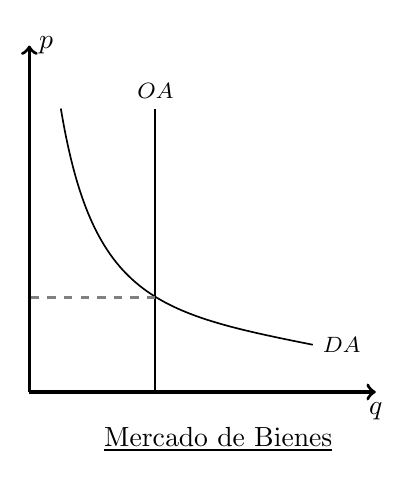
\begin{tikzpicture}[scale=0.4]
\draw[very thick,<-] (0,11)--(0,0);
\draw[very thick,->] (0,0)--(11,0) node[below]{$q$};
\node[right] at (0,11) {$p$};


\node[] at(6,-1.5) {\underline{Mercado de Bienes}};
\draw[semithick] (1,9).. controls (2,3) and (4, 2.5) .. (9, 1.5) node [right]{\footnotesize $DA$};
\draw[semithick](4, 0)--(4, 9) node [above]{\footnotesize $OA$};

\draw[thick, gray, dashed] (4,3)--(0,3);
\end{tikzpicture}
\end{center}
     \end{minipage}
  %  \hfill
    \begin{minipage}[b]{0.45\textwidth}
    \begin{center}
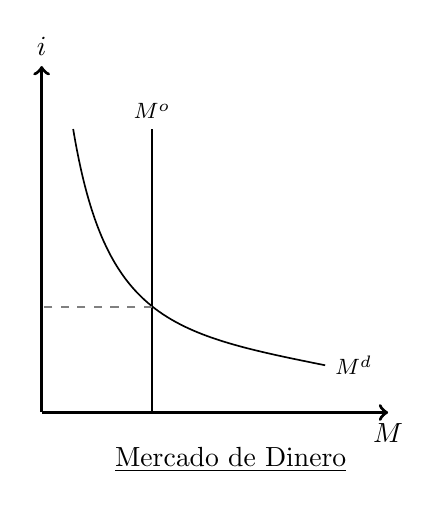
\begin{tikzpicture}[scale=0.4]
\draw[very thick,<-] (0,11) node[above]{$i$}--(0,0);
\draw[very thick,->] (0,0)--(11,0) node[below]{$M$};
\node[right] at (0,11) {};

\node[] at(6,-1.5) {\underline{Mercado de Dinero}};
\draw[semithick] (1,9).. controls (2,3) and (4, 2.5) .. (9, 1.5) node [right]{\footnotesize $M^{d}$};
\draw[semithick](3.5, 0)--(3.5, 9) node [above]{\footnotesize $M^{o}$};

 \draw[thick, gray, dashed] (3.5,3.35)--(0,3.35);

\end{tikzpicture}
\end{center}
    \end{minipage}
\end{center}
\vspace{0.7cm}
\caption{\textbf{Configuración clásica}}
\label{fig:C35.3}
\end{figure}
\end{center} 
  
  
\end{frame}



\begin{frame}{El mecano en el mundo keynesiano}
 
 \begin{center}
\begin{figure}[H]
\renewcommand{\figurename}{Figure}
\begin{center}
    \begin{minipage}[b]{0.45\textwidth}
        \begin{center}
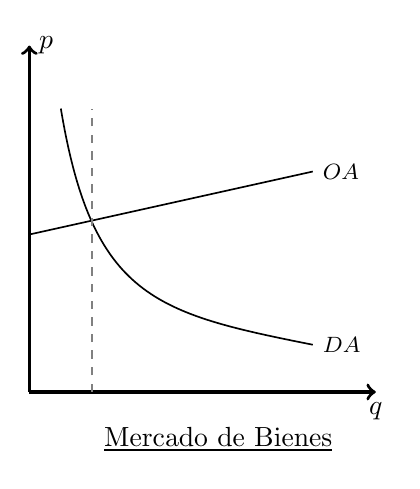
\begin{tikzpicture}[scale=0.4]
\draw[very thick,<-] (0,11)--(0,0);
\draw[very thick,->] (0,0)--(11,0) node[below]{$q$};
\node[right] at (0,11) {$p$};


\node[] at(6,-1.5) {\underline{Mercado de Bienes}};
\draw[semithick] (1,9).. controls (2,3) and (4, 2.5) .. (9, 1.5) node [right]{\footnotesize $DA$};
\draw[semithick](0, 5)--(9,7) node [right]{\footnotesize $OA$};
 \draw[thick, gray, dashed] (2,0)--(2,9);
\end{tikzpicture}
\end{center}
     \end{minipage}
  %  \hfill
    \begin{minipage}[b]{0.45\textwidth}
    \begin{center}
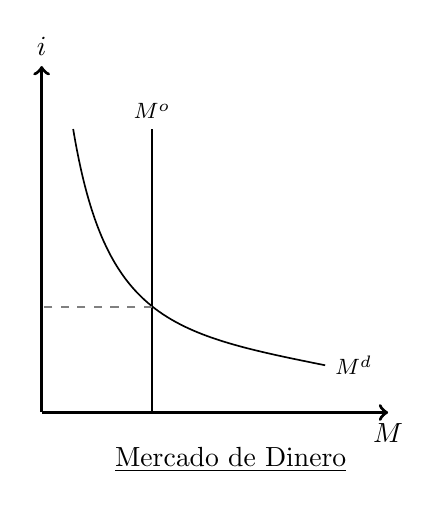
\begin{tikzpicture}[scale=0.4]
\draw[very thick,<-] (0,11) node[above]{$i$}--(0,0);
\draw[very thick,->] (0,0)--(11,0) node[below]{$M$};
\node[right] at (0,11) {};


\node[] at(6,-1.5) {\underline{Mercado de Dinero}};
\draw[semithick] (1,9).. controls (2,3) and (4, 2.5) .. (9, 1.5) node [right]{\footnotesize $M^{d}$};
\draw[semithick](3.5, 0)--(3.5, 9) node [above]{\footnotesize $M^{o}$};

 \draw[thick, gray, dashed] (3.5,3.35)--(0,3.35);

\end{tikzpicture}
\end{center}
    \end{minipage}
\end{center}
\vspace{0.7cm}
\caption{\textbf{Configuración keynesiana}}
\label{fig:C35.4}
\end{figure}
\end{center} 
 
\end{frame}



%---------------------------------------------------------------------------%
%---------------------------------------------------------------------------%

\begin{frame}{}
\centering 	\huge \textbf{Política monetaria} 
\vspace{2mm}
\hrule
\end{frame}
%---------------------------------------------------------------------------%
%---------------------------------------------------------------------------%

\begin{frame}{Política Monetaria en el mundo clásico}
 
 \begin{center}
\begin{figure}[H]
\renewcommand{\figurename}{Figure}
\begin{center}
    \begin{minipage}[b]{0.45\textwidth}
        \begin{center}
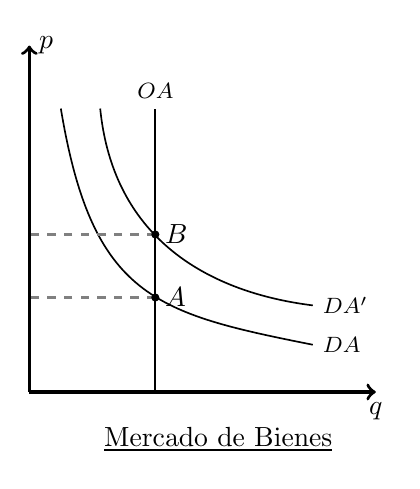
\begin{tikzpicture}[scale=0.4]
\draw[very thick,<-] (0,11)--(0,0);
\draw[very thick,->] (0,0)--(11,0) node[below]{$q$};
\node[right] at (0,11) {$p$};

\node[] at(6,-1.5) {\underline{Mercado de Bienes}};
\draw[semithick] (1,9).. controls (2,3) and (4, 2.5) .. (9, 1.5) node [right]{\footnotesize $DA$};
\draw[semithick] (2.25,9).. controls (2.75,4) and (7, 3) .. (9, 2.75) node [right]{\footnotesize $DA'$};
\draw[semithick](4, 0)--(4, 9) node [above]{\footnotesize $OA$};
\draw[thick, gray, dashed] (4,3)--(0,3);
\draw[thick, gray, dashed] (4,5)--(0,5);
   \draw[fill] (4,3) circle [radius =0.11] node[right] {$A$}; 
      \draw[fill] (4,5) circle [radius =0.11] node[right] {$B$}; 
\end{tikzpicture}
\end{center}
     \end{minipage}
  %  \hfill
    \begin{minipage}[b]{0.45\textwidth}
    \begin{center}
\begin{tikzpicture}[scale=0.4]
\draw[very thick,<-] (0,11) node[above]{$i$}--(0,0);
\draw[very thick,->] (0,0)--(11,0) node[below]{$M$};
\node[right] at (0,11) {};


\node[] at(6,-1.5) {\underline{Mercado de Dinero}};
\draw[semithick] (1,9).. controls (2,3) and (4, 2.5) .. (9, 1.5) node [right]{\footnotesize $M^{d}$};
\draw[semithick] (2.25,9).. controls (2.75,4) and (7, 3) .. (9, 2.75) node [right]{\footnotesize $M^{d^{'}}$};
\draw[semithick](3.5, 0)--(3.5, 9) node [above]{\footnotesize $M^{o}$};
 \draw[semithick](6.5, 0)--(6.5, 9) node [above]{\footnotesize $M^{o}'$};
 \draw[thick, gray, dashed] (6.5,3.35)--(0,3.35);
   \draw[fill] (3.5,3.35) circle [radius =0.11] node[right] {$A$}; 
      \draw[fill] (6.5,3.35) circle [radius =0.11] node[right] {$B$}; 
\end{tikzpicture}
\end{center}
    \end{minipage}
\end{center}
\vspace{0.7cm}
\caption{\textbf{Política monetaria en el mundo clásico}}
\label{fig:C35.4}
\end{figure}
\end{center} 

 
\end{frame}



%---------------------------------------------------------------------------%

%\begin{frame}{Política monetaria en el mundo clásico}

%    \begin{itemize}
%        \item “Aumenta la demanda agregada” al meter liquidez en el sistema 
%       \item Pero el producto está dado por la oferta agregada
%        \item Por lo que el aumento en la demanda presiona sobre los precios
%        \item Lo que lleva a que los precios aumenten proporcionalmente a lo que aumentó la cantidad de dinero
%       \item Oferta y demanda de dinero simplemente se corren para encontrar el equilibrio en el mismo nivel.
%        \item $\uparrow M V(i)=\uparrow P Y$ 
  %     \item Dicotomía clásica (“Neutralidad del dinero”) - $(Y \text { e } i \text { constante, } M \rightarrow P)$
  %  \end{itemize}
    

%\end{frame}

%---------------------------------------------------------------------------%

\begin{frame}{¿Cómo se recauda el impuesto inflacionario?}

    \begin{itemize}
        \item El gobierno emite un dinero
        \item Esto aumenta lo precios
        \item Ese aumento de precios hace que los tenedores de pesos puedan consumir menos.
        \item De esa manera parte del producto lo apropia el Estado
    \end{itemize}
    
\end{frame}

%---------------------------------------------------------------------------%

\begin{frame}{Política monetaria en el mundo keynesiano}
  
\begin{center}
\begin{figure}[H]
\renewcommand{\figurename}{Figure}
\begin{center}
    \begin{minipage}[b]{0.45\textwidth}
        \begin{center}
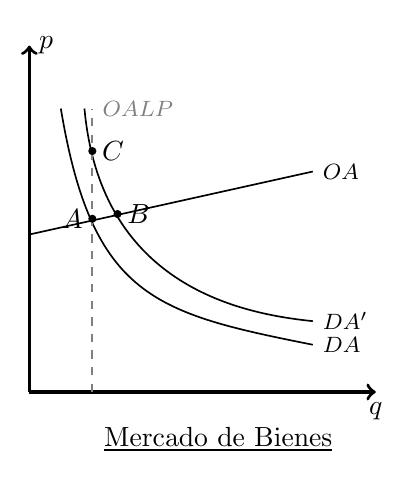
\begin{tikzpicture}[scale=0.4]
\draw[very thick,<-] (0,11)--(0,0);
\draw[very thick,->] (0,0)--(11,0) node[below]{$q$};
\node[right] at (0,11) {$p$};


\node[] at(6,-1.5) {\underline{Mercado de Bienes}};
\draw[semithick] (1,9).. controls (2,3) and (4, 2.5) .. (9, 1.5) node [right]{\footnotesize $DA$};
\draw[semithick] (1.75,9).. controls (2.25,3.5) and (6.5,2.5) .. (9, 2.25) node [right]{\footnotesize $DA'$};
\draw[semithick](0, 5)--(9, 7) node [right]{\footnotesize $OA$};
 \draw[thick, gray, dashed] (2,0)--(2,9) node [right]{\footnotesize $OALP$};
   \draw[fill] (2,5.5) circle [radius =0.11] node[left] {$A$}; 
  \draw[fill] (2.8,5.65) circle [radius =0.11] node[right] {$B$}; 
  \draw[fill] (2,7.65) circle [radius =0.11] node[right] {$C$}; 
 
\end{tikzpicture}
\end{center}
     \end{minipage}
  %  \hfill
    \begin{minipage}[b]{0.45\textwidth}
    \begin{center}
\begin{tikzpicture}[scale=0.4]
\draw[very thick,<-] (0,11) node[above]{$i$}--(0,0);
\draw[very thick,->] (0,0)--(11,0) node[below]{$M$};
\node[right] at (0,11) {};

\node[] at(6,-1.5) {\underline{Mercado de Dinero}};
\draw[semithick] (1,9).. controls (2,3) and (4, 2.5) .. (9, 1.5) node [right]{\footnotesize $M^{d}$};
\draw[semithick] (1.75,9).. controls (2.25,3) and (6.75, 2.5) .. (9, 2.15) node [right]{\footnotesize $M^{d^{'}}$};
\draw[semithick, gray, dashed] (2.5,9).. controls (2.25,3.7) and (6.75, 3.5) .. (9, 2.9) node [right]{\footnotesize $M^{d^{''}}$};
\draw[semithick](3.5, 0)--(3.5, 9) node [above]{\footnotesize $M^{o}$};
 \draw[semithick](6.5, 0)--(6.5, 9) node [above]{\footnotesize $M^{o}'$};
 \draw[semithick](6.5, 0)--(6.5, 9) node [above]{\footnotesize $M^{o}'$};


 \draw[thick, gray, dashed] (3.5,3.35)--(0,3.35);
 \draw[thick, gray, dashed] (6.5,2.625)--(0,2.625);

  \draw[fill] (3.35,3.35) circle [radius =0.11] node[right] {$A$}; 
  \draw[fill] (6.5,2.625) circle [radius =0.11] node[right] {$B$}; 
   \draw[fill] (6.5,3.35) circle [radius =0.11] node[right] {$C$}; 
\end{tikzpicture}
\end{center}
    \end{minipage}
\end{center}
\vspace{0.7cm}
\caption{\textbf{Política monetaria en el mundo keynesiano}}
\label{fig:C35.5}
\end{figure}
\end{center}   
\end{frame}


%---------------------------------------------------------------------------%



%\begin{frame}{Política monetaria en el mundo keynesiano}

  %  \begin{itemize}
  %      \item Ahora “aumenta la demanda agregada” pero ahora esto baja la tasa de interés y lleva a un aumento en el producto.
  %      \item El dinero excedente reduce la tasa de interés en el mercado de crédito
  %     \item $\uparrow M V(i) \downarrow=\bar{P} Y \uparrow$
  %     \item (P constante $, M \rightarrow i, i \rightarrow Y)$
  %  \end{itemize}
  

%\end{frame}

%---------------------------------------------------------------------------%

\begin{frame}{¿Es efectiva la política monetaria?}

    \begin{itemize}
        \item Depende del contexto si los precios se mueven rápido no va a lograr mucho, si los precios son "rígidos" tendrá más impacto. 
        \item En definitiva es una cuestión de contexto.
        \item Podríamos presumir que la política monetaria en Argentina sería menos efectiva que en los EEUU

    \end{itemize}
    
\end{frame}

%---------------------------------------------------------------------------%

\begin{frame}{¿Cómo funcionan la política monetaria y la fiscal?}
    
    \centering\includegraphics[width=11cm]{P81.png}\

\end{frame}

%---------------------------------------------------------------------------%

%\begin{frame}{Maneras de pensar la política monetaria}
    

%    \begin{itemize}
%        \item La política monetaria se apoya en un “ancla nominal”: tipo de cambio, cantidad de dinero o metas de inflación.
%        \item ¿Discreción o reglas?
       
%        \item Mas discreción lleva a más inflación
%        \item Más preocupación por el producto lleva a más inflación
%            \item Paradoja: cuanto más creíble es un banquero central, más discrecional puede ser
%            \item  Por eso el 28D fue tan trascendental en la presidencia de Macri. 
            
 %       \end{itemize}

 

%\end{frame}

%---------------------------------------------------------------------------%
%---------------------------------------------------------------------------%

\begin{frame}{}
\centering 	\huge \textbf{Política fiscal} 
\vspace{2mm}
\hrule
\end{frame}
%---------------------------------------------------------------------------%
%---------------------------------------------------------------------------%

\begin{frame}{¿Cómo funciona la política fiscal?}
    
    \begin{itemize}
        \item El análisis de la política fiscal es mucho más complejo por una serie de motivos:
        \begin{itemize}
            \item Aumenta la demanda agregada. 
            \item Pero cuando se analiza la política fiscal debemos tener en cuenta que la misma requiere financiamiento.
            \item Lo que genera efectos expulsión (“crowding out”) (director o vía la tasa de interés).
        \end{itemize}

    \end{itemize}

\end{frame}

%---------------------------------------------------------------------------%

\begin{frame}{El financiamiento además puede ser diferente}
    
    \begin{itemize}
        \item Existen tres mecanismos básicos para financiar la política fiscal:
        \begin{itemize}
            \item Emisión monetaria 
            \item Impuestos
            \item Deuda interna
         
        \end{itemize}
        \item Cada uno de estos implicará distintos mecanismos sobre la demanda agregada
    \end{itemize}

\end{frame}

%---------------------------------------------------------------------------%
\begin{frame}{El efecto “financiamiento” sobre el consumo}
    
    \begin{itemize}
        \item Supongamos primero que aumenta el gasto público financiado enteramente con impuestos: ¿cuánto cae el consumo privado?
        \begin{itemize}
            \item Cae el consumo que esos impuestos desplazan. 
            \item Si los impuestos son permanentes la caída del consumo debiera ser el 100\% del aumento de los impuestos.
            \item La caída del consumo es menor si se piensa que es transitorio.
            \item Lo cierto es que el efecto de la política fiscal se modera sustancialmente cuando se tiene en cuenta el financiamiento.
        \end{itemize}
        \item Supongamos ahora que aumenta el gasto público financiado con deuda: ¿cuánto cae el consumo privado?
        \begin{itemize}
            \item En principio podríamos pensar que nada.
            \item Pero igual que si financia con impuestos si existe “equivalencia ricardiana”.
            \item Y hay crowding out también si hay un aumento en la tasa de interés
        \end{itemize}
    \end{itemize}

\end{frame}

%---------------------------------------------------------------------------%

\begin{frame}{Ejemplo de equivalencia ricardiana}
    
    \begin{itemize}
        \item Supongamos dos periodos ingresos de 1000 y 1000
        \item El gobierno va a gastar 100 y 100 
        \item Lo financia con deuda en el primer periodo y la tasa de interés es 10\%.
        \item El agente enfrenta impuestos de 0 y 210.
        \item Si consume su ingreso consumiría 1000 y 790. 
        \item ¿Qué pasa si ahorra 100 en el primero período?
    \item Ahora puede consumir 900 y 900
    \item Que es mejor que 1000 y 790.
    \item Pero 900 y 900 es lo mismo que si el gobierno hubiera financiado los 100 con impuestos! 
        
        
    \end{itemize}

\end{frame}

%---------------------------------------------------------------------------%

\begin{frame}{El efecto expulsión (“crowding out”)}

    \begin{itemize}
    \footnotesize\item Tiene dos componentes:
        \begin{itemize}
        \scriptsize\item El menor ingreso neto implica menor ahorro lo cual reduce la oferta de fondos prestables
        \scriptsize\item La mayor demanda de fondos públicos (si se financia con deuda) aumenta la demanda de fondos prestables sube la tasa de interés y por ende debilita la inversión
        \scriptsize\end{itemize}
    \end{itemize}
    
    \vspace{0.2cm}
    
    \centering\includegraphics[width=7cm]{P87.png}\

\end{frame}

%---------------------------------------------------------------------------%

%\begin{frame}{El efecto expulsión en un mundo ricardiano}

%    \begin{itemize}
%    \scriptsize\item A menos que el financiamiento genere un aumento del ahorro privado.
%    \scriptsize\item Por ejemplo, un aumento del gasto publico financiado con deuda en un contexto Ricardiano no afecta la inversión porque la tasa no cambia.
%    \scriptsize\item Pero la caída del consumo diluye el efecto sobre la demanda agregada.

%\end{itemize}
    
%    \vspace{0.2cm}
    
%    \centering\includegraphics[width=7cm]{P88.png}\

%\end{frame}

%---------------------------------------------------------------------------%


\begin{frame}{¿Pero existe ese fenómeno Ricardiano? I}

     \begin{center}
         Correlación entre deuda pública y activos financieros netos acumulados por los hogares
     \end{center}

     \centering\includegraphics[width=11cm]{P91b.png}\  

     \begin{center}
         Grennes y Strazds (2013) en base a datos de Eurostat
     \end{center}

\end{frame}

%---------------------------------------------------------------------------%

\begin{frame}{¿Pero existe ese fenómeno Ricardiano? II}

    

     \centering\includegraphics[width=11cm]{C36.11.png}\  
\begin{itemize}
    \item El caso sudafricano reciente
    \end{itemize}

\end{frame}

%---------------------------------------------------------------------------%


\begin{frame}{¿Cuándo tiene, entonces, la política fiscal un efecto sobre la demanda agregada?}

    \begin{itemize}
    \item Cuando no hay una reducción equivalente del consumo privado.
    \end{itemize}
     \vspace{3mm}
    
    \centering\includegraphics[width=6cm]{P95b.png}\

\end{frame}

%---------------------------------------------------------------------------%


\begin{frame}{Expansión fiscal c/impuestos (permanentes/clásico)}
   
 \begin{center}
\begin{figure}[H]
\renewcommand{\figurename}{Figure}
\begin{center}
    \begin{minipage}[b]{0.45\textwidth}
        \begin{center}
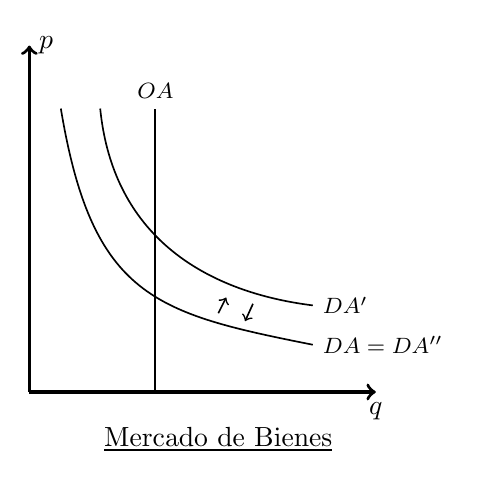
\begin{tikzpicture}[scale=0.4]
\draw[very thick,<-] (0,11)--(0,0);
\draw[very thick,->] (0,0)--(11,0) node[below]{$q$};
\node[right] at (0,11) {$p$};

\node[] at(6,-1.5) {\underline{Mercado de Bienes}};
\draw[semithick] (1,9).. controls (2,3) and (4, 2.5) .. (9, 1.5) node [right]{\footnotesize $DA=DA''$};
\draw[semithick] (2.25,9).. controls (2.75,4) and (7, 3) .. (9, 2.75) node [right]{\footnotesize $DA'$};
\draw[semithick](4, 0)--(4, 9) node [above]{\footnotesize $OA$};
\draw[semithick, ->] (6,2.5)--(6.25,3);
\draw[semithick, <-] (6.85,2.25)--(7.1,2.8);
%\draw[thick, gray, dashed] (4,3)--(0,3);
\end{tikzpicture}
\end{center}
     \end{minipage}
  %  \hfill
    \begin{minipage}[b]{0.45\textwidth}
    \begin{center}
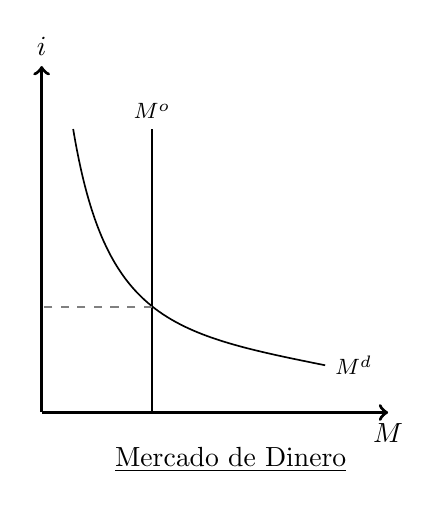
\begin{tikzpicture}[scale=0.4]
\draw[very thick,<-] (0,11) node[above]{$i$}--(0,0);
\draw[very thick,->] (0,0)--(11,0) node[below]{$M$};
\node[right] at (0,11) {};

\node[] at(6,-1.5) {\underline{Mercado de Dinero}};
\draw[semithick] (1,9).. controls (2,3) and (4, 2.5) .. (9, 1.5) node [right]{\footnotesize $M^{d}$};
\draw[semithick](3.5, 0)--(3.5, 9) node [above]{\footnotesize $M^{o}$};

 \draw[thick, gray, dashed] (3.5,3.35)--(0,3.35);

\end{tikzpicture}
\end{center}
    \end{minipage}
\end{center}
\vspace{0.7cm}
\caption{\textbf{Política fiscal financiada con un aumento permanente de los impuestos}}
\label{fig:C36.2}
\end{figure}
\end{center}   
   
\end{frame}

%---------------------------------------------------------------------------%

%\begin{frame}{Expansión fiscal c/impuestos (permanentes/clásico)}
   
%   \begin{itemize}
%       \item No hay efectos: lo que el gobierno gasta, la gente lo deja de gastar.
%       \item La demanda agregada no se modifica
%       \item No importa como es la curva de oferta
%       \item Es decir el resultado es el mismo en el mundo clásico o keynesiano.
%   \end{itemize}
    
%\end{frame}

%---------------------------------------------------------------------------%



%---------------------------------------------------------------------------%


%---------------------------------------------------------------------------%

\begin{frame}{Expansión fiscal c/ impuestos transitorios/clásico}
   
\begin{center}
\begin{figure}[H]
\renewcommand{\figurename}{Figure}
\begin{center}
    \begin{minipage}[b]{0.45\textwidth}
        \begin{center}
\begin{tikzpicture}[scale=0.4]
\draw[very thick,<-] (0,11)--(0,0)0;
\draw[very thick,->] (0,0)--(11,0) node[below]{$q$};
\node[right] at (0,11) {$p$};
\node[] at(6,-1.5) {\underline{Mercado de Bienes}};
\draw[semithick] (1,9).. controls (2,3) and (4, 2.5) .. (9, 1.5) node [right]{\footnotesize $DA$};
\draw[semithick] (2.25,9).. controls (2.75,4) and (7, 3) .. (9, 2.75) node [right]{\footnotesize $DA'$};
\draw[semithick](4, 0)--(4, 9) node [above]{\footnotesize $OA$};
\draw[thick, gray, dashed] (7.5,3)--(0,3);
\draw[thick, gray, dashed] (4,5)--(0,5);
\draw[fill] (7.5,3) circle [radius =0.11] node[above] {\scriptsize A};
\draw[fill] (4,5) circle [radius =0.11] node[right] {\scriptsize B};
\end{tikzpicture}
\end{center}
     \end{minipage}
  %  \hfill
    \begin{minipage}[b]{0.45\textwidth}
    \begin{center}
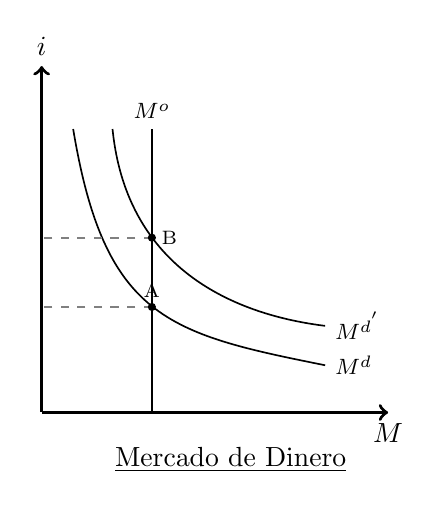
\begin{tikzpicture}[scale=0.4]
\draw[very thick,<-] (0,11) node[above]{$i$}--(0,0);
\draw[very thick,->] (0,0)--(11,0) node[below]{$M$};
\node[right] at (0,11) {};
\node[] at(6,-1.5) {\underline{Mercado de Dinero}};
\draw[semithick] (1,9).. controls (2,3) and (4, 2.5) .. (9, 1.5) node [right]{\footnotesize $M^{d}$};
\draw[semithick] (2.25,9).. controls (2.75,4) and (7, 3) .. (9, 2.75) node [right]{\footnotesize $M^{d^{'}}$};
\draw[semithick](3.5, 0)--(3.5, 9) node [above]{\footnotesize $M^{o}$};
 \draw[thick, gray, dashed] (3.5,3.35)--(0,3.35);
 \draw[thick, gray, dashed] (3.5,5.55)--(0,5.55);
 %\draw[semithick, ->] (6,2.5)--(6.25,3);
%\draw[semithick, <-] (6.85,2.25)--(7.1,2.8);
\draw[fill] (3.5,3.35) circle [radius =0.11] node[above] {\scriptsize A};
\draw[fill] (3.5,5.55) circle [radius =0.11] node[right] {\scriptsize B};

\end{tikzpicture}
\end{center}
    \end{minipage}
\end{center}
\vspace{0.7cm}
\caption{\textbf{Política fiscal financiada con un aumento transitorio de los impuestos - Clásico}}
\label{fig:C36.2}
\end{figure}
\end{center} 

\end{frame}

%---------------------------------------------------------------------------%
%\begin{frame}{Expansión fiscal c/impuestos transitorios/clásico}
   
%   \begin{itemize}
%       \item La reversión de la demanda agregada no es plena
%       \item El exceso de demanda empuja los precios para arriba
%       \item Eso aumenta la demanda de dinero empujando para arriba la tasa de interés
  
%    \item A la postre el crowding out es pleno
  
%   \end{itemize}
    
%\end{frame}
%---------------------------------------------------------------------------%
\begin{frame}{Expansión fiscal c/impuestos transitorios/keynesiano}
    
\begin{center}
\begin{figure}[H]
\renewcommand{\figurename}{Figure}
\begin{center}
    \begin{minipage}[b]{0.45\textwidth}
        \begin{center}
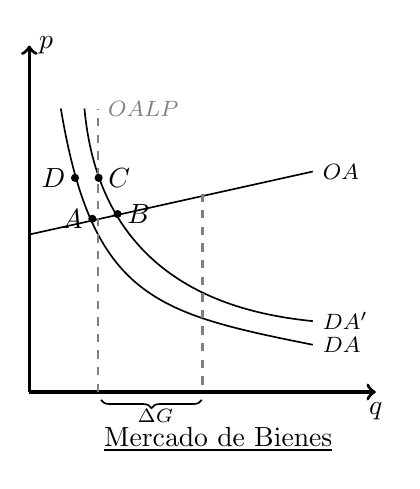
\begin{tikzpicture}[scale=0.4]
\draw[very thick,<-] (0,11)--(0,0);
\draw[very thick,->] (0,0)--(11,0) node[below]{$q$};
\node[right] at (0,11) {$p$};

\node[] at(6,-1.5) {\underline{Mercado de Bienes}};
\draw[semithick] (1,9).. controls (2,3) and (4, 2.5) .. (9, 1.5) node [right]{\footnotesize $DA$};
%\draw[semithick] (2.25,9).. controls (2.75,4) and (7, 3) .. (9, 2.75) node [right]{\footnotesize $DA'$};
\draw[semithick] (1.75,9).. controls (2.25,3.5) and (6.5,2.5) .. (9, 2.25) node [right]{\footnotesize $DA'$};
\draw[semithick](0, 5)--(9, 7) node [right]{\footnotesize $OA$};
\draw [semithick,decorate,decoration={brace,amplitude=3pt, mirror},xshift=5pt,yshift=0pt](2.1,-0.25) -- (5.3,-0.25);
\draw (4,-0.75) node[]{\scriptsize $\Delta G $};
\draw[thick, gray, dashed] (2.175,0)--(2.175,9) node [right]{\footnotesize $OALP$};;
\draw[thick, gray, dashed] (5.5,6.3)--(5.5,0);
\draw[fill] (2,5.5) circle [radius =0.11] node[left] {$A$}; 
\draw[fill] (2.8,5.65) circle [radius =0.11] node[right] {$B$}; 
\draw[fill] (2.2,6.8) circle [radius =0.11] node[right] {$C$}; 
\draw[fill] (1.45,6.8) circle [radius =0.11] node[left] {$D$}; 
\end{tikzpicture}
\end{center}
     \end{minipage}
  %  \hfill
    \begin{minipage}[b]{0.45\textwidth}
    \begin{center}
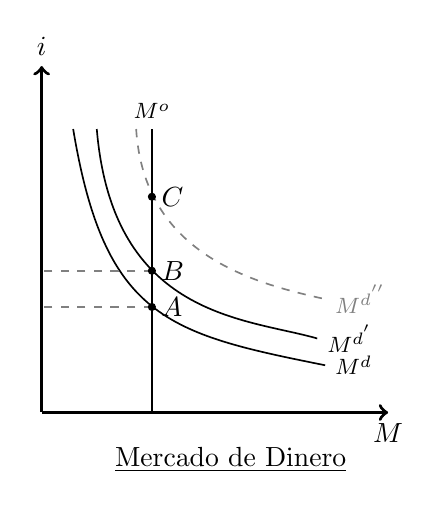
\begin{tikzpicture}[scale=0.4]
\draw[very thick,<-] (0,11) node[above]{$i$}--(0,0);
\draw[very thick,->] (0,0)--(11,0) node[below]{$M$};
\node[right] at (0,11) {};
\node[] at(6,-1.5) {\underline{Mercado de Dinero}};
\draw[semithick] (1,9).. controls (2,3) and (4, 2.5) .. (9, 1.5) node [right]{\footnotesize $M^{d}$};
\draw[semithick] (1.75,9).. controls (2.25,3) and (6.5, 3) .. (8.75, 2.35) node [right]{\footnotesize $M^{d^{'}}$};
\draw[semithick, gray, dashed] (3,9).. controls (3.25,5) and (6.75,4.1) .. (9,3.6) node [right]{\footnotesize $M^{d^{''}}$};
\draw[semithick](3.5, 0)--(3.5, 9) node [above]{\footnotesize $M^{o}$};
\draw[thick, gray, dashed] (3.5,3.35)--(0,3.35);
\draw[thick, gray, dashed] (3.5,4.5)--(0,4.5);
\draw[fill] (3.5,3.35) circle [radius =0.11] node[right] {$A$}; 
\draw[fill] (3.5,4.5) circle [radius =0.11] node[right] {$B$}; 
\draw[fill] (3.5,6.85) circle [radius =0.11] node[right] {$C$};
\end{tikzpicture}
\end{center}
    \end{minipage}
\end{center}
\vspace{0.7cm}
\caption{\textbf{Política fiscal financiada con un aumento transitorio de los impuestos - Keynesiano}}
\label{fig:C36.4}
\end{figure}
\end{center} 

\end{frame}


%---------------------------------------------------------------------------%
%\begin{frame}{Expansión fiscal c/impuestos transitorios/keynesiano}
   
%   \begin{itemize}
%       \item La reversión de la demanda agregada no es plena
%       \item El exceso de demanda hace subir el producto 
%       \item Eso aumenta la demanda de dinero empujando para arriba la tasa de interés 
%        \item La tasa de interés sube menos (que en el caso clásico) y el producto se expande 
%        \item Los precios empiezan  a subir, cuando la politica se revierte, se pasa por una fase recesiva. 
%   \end{itemize}
    
%\end{frame}


%---------------------------------------------------------------------------%


\begin{frame}{¿Cómo funciona la política fiscal financiada con deuda doméstica?}

    \begin{itemize}
    \item Acá el punto clave es si los agentes anticipan la carga impositiva que implica la mayor deuda
    \item Si se anticipan los impuestos necesarios para pagar esta deuda, es igual que el caso anterior (equivalencia ricardiana)
    \item En la práctica se encuentra que el ahorro responde a la deuda, pero que la compensación no es plena
    \item En tanto el efecto no es de compensación plena, hay un efecto expansivo en la demanda agregada (con efecto sobre el producto en un mundo keynesiano)

    \end{itemize}

\end{frame}



%---------------------------------------------------------------------------%

%\begin{frame}{Expansión fiscal con deuda no ricardianos, clásico}

%\begin{center}
%\begin{figure}[H]
%\renewcommand{\figurename}{Figure}
%\begin{center}
%    \begin{minipage}[b]{0.45\textwidth}
%        \begin{center}
%\begin{tikzpicture}[scale=0.4]
%\draw[very thick,<-] (0,11)--(0,0);
%\draw[very thick,->] (0,0)--(11,0) node[below]{$q$};
%\node[right] at (0,11) {$p$};

%\node[] at(6,-1.5) {\underline{Mercado de Bienes}};
%\draw[semithick] (1,9).. controls (2,3) and (4, 2.5) .. (9, 1.5) node [right]{\footnotesize $DA$};
%\draw[semithick] (2.25,9).. controls (2.75,4) and (7, 3) .. (9, 2.75) node [right]{\footnotesize $DA'$};
%\draw[semithick] (3.25,9).. controls (3.25,5) and (8.5, 3.75) .. (9, 3.75) node [right]{\footnotesize $DA'''$};
%\draw[semithick](4, 0)--(4, 9) node [above]{\footnotesize $OA$};
%\draw[thick, gray, dashed] (7.5,3)--(0,3);
%\draw[thick, gray, dashed] (4,5)--(0,5);
%\draw[fill] (7.5,3) circle [radius =0.11] node[above] {\scriptsize A};
%\draw[fill] (4,5) circle [radius =0.11] node[right] {\scriptsize B};
%\draw[fill] (4,6.5) circle [radius =0.11] node[left] {\scriptsize C}; 
%\end{tikzpicture}
%\end{center}
 %    \end{minipage}
  %  \hfill
 %   \begin{minipage}[b]{0.45\textwidth}
 %   \begin{center}
%\begin{tikzpicture}[scale=0.4]
%\draw[very thick,<-] (0,11) node[above]{$i$}--(0,0);
%\draw[very thick,->] (0,0)--(11,0) node[below]{$M$};
%\node[right] at (0,11) {};
%\node[] at(6,-1.5) {\underline{Mercado de Dinero}};
%\draw[semithick] (1,9).. controls (2,3) and (4, 2.5) .. (9, 1.5) node [right]{\footnotesize $M^{d}$};
% \draw[semithick] (2.25,9).. controls (2.75,4) and (7, 3) .. (9, 2.75) node [right]{\footnotesize $M^{d^{'}}$};
%\draw[semithick] (1.75,9).. controls (2.25,2.75) and (6.25, 2.75) .. (9, 2.25) node [right]{\footnotesize $M^{d^{'}}$};
%\draw[semithick] (2.25,9).. controls (2.75,4) and (7, 3) .. (9, 2.75) node [right]{\footnotesize $M^{d^{'}}$};
%\draw[semithick](3.5, 0)--(3.5, 9) node [above]{\footnotesize $M^{o}$};
% \draw[semithick](6.5, 0)--(6.5, 9) node [above]{\footnotesize $M^{s}'$};
%  \draw[thick, gray, dashed] (3.5,3.35)--(-3.5,3.35);
%  \draw[thick, gray, dashed] (3.5,5.55)--(-3.5,5.55);
%\draw[thick, gray, dashed] (3.5,3.35)--(0,3.35);
% \draw[thick, gray, dashed] (3.5,5.55)--(0,5.55);
% \draw[thick, gray, dashed] (3.5,4.25)--(0,4.25);
%\draw[fill] (3.5,3.4) circle [radius =0.11] node[right] {\scriptsize A};  
%\draw[fill] (3.5,5.55) circle [radius =0.11] node[left] {\scriptsize B};  
%\draw[fill] (3.5,5.55) circle [radius =0.11] node[right] {\scriptsize B};  
%\end{tikzpicture}
%\end{center}
%    \end{minipage}
%\end{center}
%\vspace{0.7cm}
%\caption{\textbf{Política fiscal financiada con deuda en el mundo clásico}}
%\label{fig:C36.7}
%\end{figure}
%\end{center} 

%\end{frame}




%---------------------------------------------------------------------------%
%\begin{frame}{Expansión fiscal/deuda/ricardianos/clásico}
   
 %  \begin{itemize}
 %      \item La reversión de la demanda agregada es plena y no se modifica
  %     \item Por consiguiente no tenemos efectos en el mercado monetario y de trabajo
   %    \item En el mercado de credito aparece la demanda del gobierno
    %    \item Pero como la gente (ricardiana) anticipa los mayores impuestos aumenta su ahorro en la misma magnitud! 
     %    \item Con lo cual no se modifican las tasas de interés 
     %     \item De hecho una de las pruebas de si hay equivalencia ricardiana es ver si las tasas de interés cambian con el déficit fiscal
   %\end{itemize}
    
%\end{frame}

%\begin{frame}{Expansión fiscal/deuda/no ricardianos/clásico}
   
 
 %  \begin{itemize}
 %      \item La reversión de la demanda agregada no es plena con lo que aumenta 
  
  %     \item Los precios aumentan eliminando el exceso de demanda
   
   
   
   %    \item Esto empuja para arriba la demanda de dinero-
    
%    \item En el mercado de crédito el gobierno aumenta la demanda incrementando la tasa de interés. 
  %       \item Como a la tasa de interés del mercado de crédito hay un exceso de oferta de dinero la tasa de interés se ubica en un valor algo menor. 
   %     \item Pero el crowding out es total
%        \item Porque lo que toma el gobierno es exacto lo que tiene que caer el consumo y la inversión. 
 %        \item En el mercado de trabajo los salarios acompañan a los precios sin efecto en el empleo 
 %  \end{itemize}
    
%\end{frame}

%---------------------------------------------------------------------------%

\begin{frame}{Expansión fiscal con deuda no ricardianos, keynesiano}


\begin{center}
\begin{figure}[H]
\renewcommand{\figurename}{Figure}
\begin{center}
    \begin{minipage}[b]{0.45\textwidth}
        \begin{center}
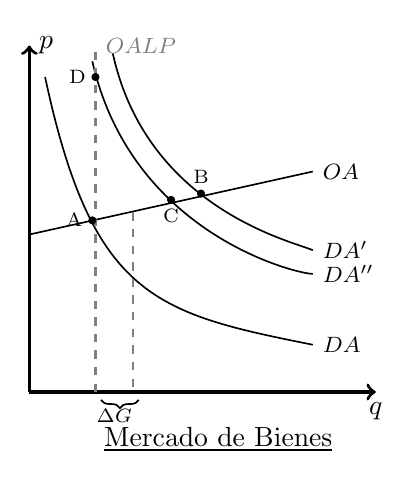
\begin{tikzpicture}[scale=0.4]
\draw[very thick,<-] (0,11)--(0,0);
\draw[very thick,->] (0,0)--(11,0) node[below]{$q$};
\node[right] at (0,11) {$p$};

\node[] at(6,-1.5) {\underline{Mercado de Bienes}};
\draw[semithick] (0.5,10).. controls (2,3) and (4, 2.5) .. (9, 1.5) node [right]{\footnotesize $DA$};

\draw[semithick] (2.65,10.75).. controls (3.75,5.75) and (8.5, 4.75) .. (9, 4.5) node [right]{\footnotesize $DA'$};
\draw[semithick] (2,10.5).. controls (3.25,5) and (8.5, 3.75) .. (9, 3.75) node [right]{\footnotesize $DA''$};
\draw[semithick](0, 5)--(9, 7) node [right]{\footnotesize $OA$};
  \draw [semithick,decorate,decoration={brace,amplitude=3pt, mirror},xshift=5pt,yshift=0pt](2.1,-0.25) -- (3.3,-0.25);
\draw (2.7,-0.75) node[]{\scriptsize $\Delta G $};

 \draw[thick, gray, dashed] (2.1,0)--(2.1,11) node [right]{\footnotesize $OALP$};
\draw[thick, gray, dashed] (3.3,5.7)--(3.3,0); 
\draw[fill] (2,5.45) circle [radius =0.11] node[left] {\scriptsize A};  
\draw[fill] (5.45,6.3) circle [radius =0.11] node[above] {\scriptsize B}; 
\draw[fill] (4.5,6.1) circle [radius =0.11] node[below] {\scriptsize C};  
\draw[fill] (2.1,10) circle [radius =0.11] node[left] {\scriptsize D};  
\end{tikzpicture}
\end{center}
     \end{minipage}
  %  \hfill
    \begin{minipage}[b]{0.45\textwidth}
    \begin{center}
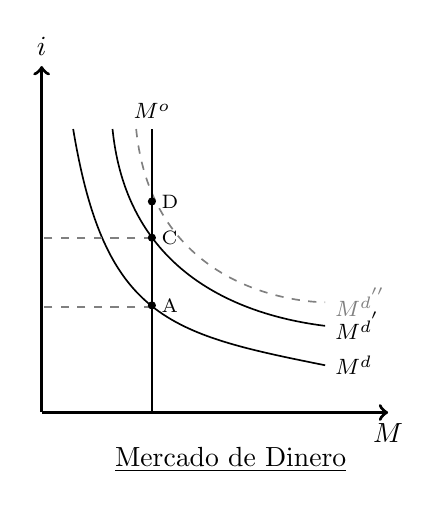
\begin{tikzpicture}[scale=0.4]
\draw[very thick,<-] (0,11) node[above]{$i$}--(0,0);
\draw[very thick,->] (0,0)--(11,0) node[below]{$M$};
\node[right] at (0,11) {};
\node[] at(6,-1.5) {\underline{Mercado de Dinero}};
\draw[semithick] (1,9).. controls (2,3) and (4, 2.5) .. (9, 1.5) node [right]{\footnotesize $M^{d}$};
\draw[semithick] (2.25,9).. controls (2.75,4) and (7, 3) .. (9, 2.75) node [right]{\footnotesize $M^{d^{'}}$};
\draw[semithick, gray, dashed] (3,9).. controls (3.5,4) and (8, 3.5) .. (9,3.5) node [right]{\footnotesize $M^{d^{''}}$};
\draw[semithick](3.5, 0)--(3.5, 9) node [above]{\footnotesize $M^{o}$};
% \draw[thick](6.5, 0)--(6.5, 9) node [above]{\footnotesize $M^{s}'$};

 \draw[thick, gray, dashed] (3.5,3.35)--(0,3.35);
 \draw[thick, gray, dashed] (3.5,5.55)--(0,5.55);
\draw[fill] (3.5,3.4) circle [radius =0.11] node[right] {\scriptsize A};  
\draw[fill] (3.5,5.55) circle [radius =0.11] node[right] {\scriptsize C};  
 \draw[fill] (3.5,6.7) circle [radius =0.11] node[right] {\scriptsize D};  
\end{tikzpicture}
\end{center}
    \end{minipage}
\end{center}
\vspace{0.7cm}
\caption{Política fiscal financiada con deuda en el mundo keynesiano}
\label{fig:C36.8}
\end{figure}
\end{center} 

\end{frame}






%---------------------------------------------------------------------------%
%\begin{frame}{Expansión fiscal/deuda/no ricardianos/keynesiano}
   
%   \begin{itemize}
 %      \item La reversión de la demanda agregada no es plena con lo que aumenta 
  %     \item Pero los precios no aumentan con lo que sube el producto
   %    \item Esto empuja para arriba la demanda de dinero y la tasa de interés nominal
    %    \item En el mercado de crédito el gobierno aumenta la demanda, el aumento en la demanda de dinero reduce algo la oferta (compensado parcialmente por el aumento del producto) 
     %   \item Acá el equilibrio es con un mayor nivel de crédito, no hay crowding out total porque el producto aumentó! 
      %   \item En el mercado de trabajo los salarios no se mueven y aumenta el empleo  
   %\end{itemize}
    
%\end{frame}


%---------------------------------------------------------------------------%

%---------------------------------------------------------------------------%
%\begin{frame}{Expansión fiscal/deuda externa/no ricardianos/keynesiano}
%    \begin{center}
%\begin{figure}[H]
%\renewcommand{\figurename}{Figure}
%\begin{center}
%\begin{tikzpicture}[scale=0.29]
%\draw[very thick,<->] (0,11) node[left]{$w$}--(0,0)--(-11,0) node[below]{$T$};
%\draw[very thick,->] (0,0)--(11,0) node[below]{$q$};
%\node[right] at (0,11) {$p$};

%\node[] at(-5,11.5) {\underline{Mercado de Trabajo}};
%\draw[semithick] (-1,9).. controls (-2,3) and (-4, 2.5) .. (-9, 1.5) node [left]{\footnotesize $DT$};
%\draw[semithick] (-2.25,9).. controls (-2.75,4) and (-7, 3) .. (-9, 2.75) node [left]{\footnotesize $DT'$};
%\draw[semithick](0,5)--(-7, 5)--(-7, 9) node [above]{\footnotesize $OT$};

%\node[] at(6,11.5) {\underline{Mercado de Bienes}};
%\draw[semithick] (1,9).. controls (2,3) and (4, 2.5) .. (9, 1.5) node [right]{\footnotesize $DA$};
%\draw[semithick] (2.25,9).. controls (2.75,4) and (7, 3) .. (9, 2.75) node [right]{\footnotesize $DA'$};
%\draw[semithick](0, 5)--(9, 5) node [right]{\footnotesize $OA$};
%   \draw [semithick,decorate,decoration={brace,amplitude=3pt, mirror},xshift=5pt,yshift=0pt](2.1,-0.25) -- (5.3,-0.25);
% \draw (4,-0.75) node[]{\scriptsize $\Delta G $};

% \draw[thick, gray, dashed] (2.175,5)--(2.175,0);
% \draw[thick, gray, dashed] (5.5,5)--(5.5,0);
%\end{tikzpicture}



%\begin{tikzpicture}[scale=0.29]
%\draw[very thick,<->] (0,11) node[above]{$i$}--(0,0)--(-11,0) node[below]{$FP$};
%\draw[very thick,->] (0,0)--(11,0) node[below]{$M$};
%\node[right] at (0,11) {};

%\node[] at(-5,-1.5) {\underline{Mercado de Crédito}};
%\draw[semithick] (-1,9).. controls (-2,3) and (-4, 2.5) .. (-9, 1.5) node [left]{\footnotesize $D_{FP}$};
%\draw[semithick] (-2.25,9).. controls (-2.75,4) and (-7, 3) .. (-9, 2.75) node [left]{\footnotesize $D_{FP}'$};
%\draw[thick,dashed] (-3.5,9)--(-3.5,0) node [below]{\footnotesize 0};

%\node[] at(6,-1.5) {\underline{Mercado de Dinero}};
%\draw[semithick] (1,9).. controls (2,3) and (4, 2.5) .. (9, 1.5) node [right]{\footnotesize $M^{d}$};
%\draw[semithick] (2.25,9).. controls (2.75,4) and (7, 3) .. (9, 2.75) node [right]{\footnotesize $M^{d^{'}}$};
%\draw[semithick](3.5, 0)--(3.5, 9) node [above]{\footnotesize $M^{o}$};
%\draw[semithick](6.5, 0)--(6.5, 9) node [above]{\footnotesize $M^{s^{'}}$};
% \draw[thick](6.5, 0)--(6.5, 9) node [above]{\footnotesize $M^{s}'$};

% \draw[thick, gray, dashed] (6.5,3.35)--(-3.5,3.35);
% \draw[thick, gray, dashed] (3.5,5.55)--(-3.5,5.55);

%\end{tikzpicture}
%\end{center}
%\vspace{0.7cm}
%\caption{\textbf{La política fiscal financiada con deuda externa y agentes no ricardianos en el mundo keynesiano}}
%\label{fig:C36.8}
%\end{figure}
%\end{center}


%\end{frame}

%---------------------------------------------------------------------------%

%\begin{frame}{Expansión fiscal/deuda externa/no ricardianos/keynesiano}
   
 %  \begin{itemize}
%       \item La reversión de la demanda agregada no es plena con lo que aumenta 
%       \item Los precios no aumentan empujando hacia arriba el producto
%       
%        \item En el mercado de crédito el gobierno aumenta la demanda, pero ojo: ahora ese aumento viene con su oferta (la deuda externa). No hay un aumento en la demanda neta.
%        \item El credito actua como aumentando los medios de pagos.
 
% \item En el mercado de trabajo los salarios no se mueven y el aumento en la demanda agregada aumenta el empleo 
% \item Es el más expansivo de los casos que vimos.
%   \end{itemize}
    
%\end{frame}

%---------------------------------------------------------------------------%

\begin{frame}{Discusión}

    \begin{itemize}
    \item Para un clásico hay poco por hacer: más vale concentrarte en lo estructural: competencia, apertura, instituciones
    \item En el mundo keynesiano, al menos hay margen, pero…
    \item A) La mayor parte de los cambios en el producto son generados por cambios en C e I, causados por los agentes individuales, inducidos por el ambiente político y las expectativas
    \item B) ¿Estamos seguros el gobierno será efectivo o incluso si actuará cuando debe actuar? 
    \end{itemize}

\end{frame}

%---------------------------------------------------------------------------%

\begin{frame}{Caveats a la política macroeconómica}

    \begin{itemize}
    \item Puede existir un problema de rezagos: las políticas pueden hacerse en un momento inadecuado.
    \item Podes pensar que podes cuando no podes (si el mundo es clásico, las políticas sólo van a resultar en inflación o deflación).
    \item Si el marco político genera gobiernos débiles, puede existir prociclicalidad fiscal o exceso de gasto.
    \item Las políticas pueden incrementar la incertidumbre.
    \item La gente puede anticipar estas políticas haciéndolas menos efectivas (inconsistencia temporal y expectativas racionales), por ejemplo si vos aumentas el dinero y la gente se da cuenta al toque, los precios suben y no lográs nada.
    \end{itemize}

\end{frame}


%\begin{frame}{Sustentabilidad Fiscal}

 %   \begin{itemize}
 %   \item Decimos que una deuda es no-sustentable si vemos que el ratio deuda PBI sube
  %   \item La deuda crece a la tasa r
  %    \item El PBI crece a la tasa g
  %     \item Decimos que la deuda esta en una trayectoria no sustentable si  
   %     \item Superávit primario (ingresos menos gastos excluyendo intereses) es menor que (r-g) Deuda/PBI. 
%     \item En Argentina por ejemplo la deuda externa era 40\% del PBI. r=5.5\% y g= 4\%. Esto implica que el déficit primario requerido era 0.6\% del PBI. 
 %   \item Pero el déficit primario recibido era 0.4\% así que no había un gran tema.
 %   \item Ahorro? 40\% sobre 100. 000 millones. 40.000 millones. En realidad 20.000 porque la mitad la tenían argentinos
 %    \item Efecto sobre el valor del capital privado: 150.000 millones
  %  \end{itemize}

%\end{frame}


\begin{frame}{Las tipologías de la macro}
\begin{table}[]
\resizebox{\textwidth}{!}{%
\begin{tabular}{|c|c|c|}
\hline
           & Shock a la oferta                                                                      & Shock a la demanda           \\ \hline
Clasico    & Teoria del ciclo real                                                                  & Inefectividad de la politica \\ \hline
Keynesiano & \begin{tabular}[c]{@{}c@{}}Conflicto entre estabilidad\\ y estabilización\end{tabular} & Divina coincidencia          \\ \hline
\end{tabular}%
}
\end{table}

\end{frame}



\begin{frame}{La curva de Phillips}
    \begin{figure} [H]   
  \centering
  \includegraphics[width=.9\textwidth]{images/C38.6.png}
  \caption{Curva de Phillips}
  \label{fig:C38.6}
\end{figure}
\begin{itemize}
    \item Representa una presunta relacion negativa entre inflacion y desempleo
    \item Solo se da en el contexto keynesiano
\end{itemize}
\end{frame} 


\begin{frame}{La curva de Phillips EEUU}
    
\begin{figure} [H]   
  \centering
  \includegraphics[width=.9\textwidth]{images/G18C.png}
  \caption{Curva de Phillips de EEUU 1900 - 1960}
  \label{fig:C38.7}
\end{figure}

\end{frame}



\begin{frame}{La historia de la macro}
    \begin{itemize}
        \item El mundo pre keynes
        \item El mundo keynesiano
        \item La revolucion de las expectativas racionales
        \item La teoria de ciclos reales
        \item El neokeynesianismo
        \item La sintesis en los modelos DSGE
    \end{itemize}
\end{frame}

\begin{frame}{El nacimiento de las expectativas racionales}
    \begin{figure} [H]
   \centering
\begin{tikzpicture}[scale=0.6]
\draw[thick,<->] (0,10) node[above]{$P$}--(0,0)--(10,0) node[right]{$Q$};
\draw(1,1)--(9,9) node[right]{$O$};
\draw(1,9)--(9,2.5) node[right]{$D$};
\draw[dashed,gray,semithick] (0,5.4)--(5.4,5.4)--(5.4,0);
\draw[dashed,gray,semithick] (0,4.1)--(7,4.1)--(7,0);
\draw[dashed,gray,semithick] (0,7)--(7,7);
\draw[dashed,gray,semithick] (4.1,0)--(4.1,4.1);
\draw[fill] (5.4,5.4) circle [radius =0.11] node[right] {\scriptsize E};  
\node[below] at (5.4,0) {\footnotesize $Q^{*}$};
\node[left] at (0,5.4) {\footnotesize $P^{*}$};
\node[left] at (0,4.1) {\footnotesize $P_{B}$};
\node[below] at (7,0) {\footnotesize $Q_{A}$};
\node[left] at (0,7) {\footnotesize $P_{A}$};
\node[below] at (4.1,0) {\footnotesize $Q_{B}$};
\draw[thick, ->,gray] (7,7)--(7,6.5);
\draw[thick, ->,gray] (7,6.5)--(7,6);
\draw[thick, ->,gray] (7,6)--(7,5.5);
\draw[thick, ->,gray] (7,5.5)--(7,5);
\draw[thick, ->,gray] (7,5)--(7,4.5);
\draw[thick, ->,gray] (7,4.5)--(7,4.1);
\draw[thick, ->,gray] (7,4.1)--(6.5,4.1);
\draw[thick, ->,gray] (6.5,4.1)--(6,4.1);
\draw[thick, ->,gray] (6,4.1)--(5.5,4.1);
\draw[thick, ->,gray] (5.5,4.1)--(5,4.1);
\draw[thick, ->,gray] (5,4.1)--(4.5,4.1);
\draw[thick, ->,gray] (4.5,4.1)--(4.1,4.1);
\draw[thick, ->,gray] (4.1,4.1)--(4.1,4.5);
\draw[thick, ->,gray] (4.1,4.5)--(4.1,5);
\draw[thick, ->,gray] (4.1,5)--(4.1,5.5);
\draw[thick, ->,gray] (4.1,5.5)--(4.1,6);
\draw[thick, ->,gray] (4.1,6)--(4.1,6.5);
\draw[thick, ->,gray] (4.1,6.5)--(4.5,6.5);
\draw[thick, ->,gray] (4.5,6.5)--(5,6.5);
\draw[thick, ->,gray] (5,6.5)--(5.5,6.5);
\draw[thick, ->,gray] (5.5,6.5)--(6,6.5);
\draw[thick, ->,gray] (6,6.5)--(6.5,6.5);
\draw[thick, ->,gray] (6.5,6.5)--(6.5,6);
\draw[thick, ->,gray] (6.5,6)--(6.5,5.5);
\draw[thick, ->,gray] (6.5,5.5)--(6.5,5);
\draw[thick, ->,gray] (6.5,5)--(6.5,4.5);
\draw[thick, ->,gray] (6.5,4.5)--(6,4.5);
\draw[thick, ->,gray] (6,4.5)--(5.5,4.5);
\draw[thick, ->,gray] (5.5,4.5)--(5,4.5);
\draw[thick, ->,gray] (5,4.5)--(4.5,4.5);
\draw[thick, ->,gray] (4.5,4.5)--(4.5,5);
\draw[thick, ->,gray] (4.5,5)--(4.5,5.5);
\draw[thick, ->,gray] (4.5,5.5)--(4.5,6.1);
\end{tikzpicture}
\caption{Modelo de la telaraña}
\label{fig:C38.8}
\end{figure}
\end{frame}


\begin{frame}{El colapso de la curva de Phillips}
    \begin{figure} [H]   
  \centering
  \includegraphics[width=1\textwidth]{images/G18B.png}
      \caption{Curva de Phillips EEUU 1960 - 1980}
  \label{fig:C38.9}
\end{figure}
\end{frame}


\begin{frame}{La curva de Phillips en Argentina}
    \begin{figure} [H]   
  \centering
  \includegraphics[width=.9\textwidth]{images/G19.png}
      \caption{Curva de Phillips Argentina 1992 - 2020}
  \label{fig:C38.10}
\end{figure}
\end{frame}


\begin{frame}{La curva de Phillips en EEUU 2008-2019}
    \begin{figure} [H]   
  \centering
  \includegraphics[width=.9\textwidth]{images/G18.png}
      \caption{Curva de Phillips EEUU 2008 - 2019}
  \label{fig:C38.11}
\end{figure}
\end{frame}



%---------------------------------------------------------------------------%
%---------------------------------------------------------------------------%


%---------------------------------------------------------------------------%

\begin{frame}{La historia de la política monetaria}
    


\begin{itemize}
    \item Pre-1939 era el patrón Oro lo que daba credibilidad a la moneda
    \item 1945-1965 El sistema de Bretton Woods, todas las monedas atadas al dolar y el dolar atado al oro. La idea de una curva de Phillips. 
    \item 1965-1982 El período de emisión sin respaldo. EEUU no puede mantener la paridad con el oro, inflación, devaluación y estanflación. La curva de Phillips se hace vertical.
    \item Volcker restablece la credibilidad de la reserva Federal, baja la inflación.
    \item Quantitative easing: el exito de credibilidad hace que la curva de Phillips se "achate" (flattening of the Phillips curve) 
    \item Vean los 25 minutos de Powell en https://www.youtube.com/watch?v=D7xw7SPIDqM&t=312s
\end{itemize}    

\end{frame}



%----

%---------------------------------------------------------------------------%



\end{document}
